\section{EXECUTIVE SUMMARY} 
xxxxxxxxxxxxxxxxxxxxxxxxx

\newpage
\section{INTRODUCTION AND BACKGROUND} 

First Light Fusion (FLF) inertial confinement fusion device is based on the nuclear reaction induced by the impact of a high-speed projectile onto a target mainly made of the fusion fuel (D-T). The use of Liquid Lithium (LL) in form of jet array in the Reactor Chamber (RC) plays a key role as tritium breeder, primary carrier of energy throughout the system, heat and nuclear shielding. \\

\noindent Taking into account that the primary carrier of energy is the LL, its circulation through the system is key to achieve the desired power cycle. This involves ensuring optimal circulation within the primary loop to maximize desired outcomes, such as purification of liquid metal from impurities introduced during operation and efficient management of tritium generated by neutron interactions for overall fuel cycle efficiency.\\

\noindent Considering the requirement to achieve an impurities control in the LL loop of the RC system, the current project studies the feasibility to separate the solid impurities from the liquid metal by means of centrifugal technologies. The first deliverable ref. \cite{SoA} explored the different technologies that potentially could address the LL loop purification.\\

\noindent The objective of the present document is to study from chemical point of view the feasibility of separate the solids impurities from the liquid media (LL), by means of Classical Nucleation Theory (CNT) where fundamental parameters such as critical radius, and its evolution by means of nucleation in the media.

\newpage
\section{SCOPE}\label{sec:scope}
The present document is part of three deliverables: the first deliverable ref. \cite{SoA} addressed the SoA of centrifugal technologies. The second deliverable (which is the current document) is focused in the chemical analysis of the impurities and the technology selection for the centrifuge device, being more specific:

\begin{itemize}
	% ---------------------------------------------------------------------------------------
	\item \textbf{Impurity and Corrosion Analysis:}
	\begin{itemize}
		\item Impurities matrix, given different source. 
		\item Corrosion products identification. 
		\item Maroni's process analysis.
	\end{itemize}
	% ---------------------------------------------------------------------------------------
	\item \textbf{Chemical analysis:}
	\begin{itemize}
		\item Particle Size Distribution (PSD) by means of CNT, for the given FLF impurities: 
		\begin{itemize}
			\item Fe
			\item Cr
			\item AlN
			\item Li2O
			\item LiQ
			\item Li2C2
		\end{itemize}
		\item Impurity critical radius time-evolution: Nucleation analysis.
		\item Homogeneous precipitation: advective-reacting diffusion equation.
	\end{itemize}
	% ---------------------------------------------------------------------------------------	
	\item \textbf{Centrifugal technology selection:}
	\begin{itemize}
		\item Single step separation stage approach.
		\item Multi-step separation stage approach.
		\item Conceptual design approach.
		\item Thermo-hydraulic analytical model.
	\end{itemize}
	% ---------------------------------------------------------------------------------------
\end{itemize}
\subsection{Exceptions} 
N/A
\subsection{Exclusions} 
N/A
\newpage
\section{STRUCTURE OF THE DOCUMENT} % ··························································

The present document it is divided in three main blocks, as per the scope section \ref{sec:scope} list. The blocks are divided by disciplines: impurities analysis SoA, chemical assessment, and engineering assessment including the thermo-hydraulic solid separator mathematical model. \\

\noindent Section \ref{sec:impurity} reviews the impurities and corrosion products in the FLF primary loop. The source of impurities are analyzed from chemical perspective in order to establish a baseline for future analysis. At the same time, a subsection is dedicated to review in the literature the corrosion products from the interaction of liquid lithium with the pipelines made SS316-Ti. The last subsection discusses the Maroni method for tritium extraction and addresses its advantages/disadvantages. \\

\noindent Section \ref{sec:chem} is deeply dedicated to the chemical analysis of the impurities, specially focused on six impurities (established by FLF: Fe, Cr, AlN, Li2O, LiQ, Li2C2) studying the Particle Size Distribution and its temporal evolution to establish the critical radius of the impurities. A specific analysis has been carried to explain the solvers and convergence benchmarks for the Ordinary Differential Equations (ODE's) system develop to understand the different phenomena. Finally, for the non-metallic impurities, a dedicated analysis is the precipitation of those impurities by means of advective-reacting diffusion equation model.  \\

\noindent Section \ref{sec:eng} studies the single and multi-step solid separators with the aim to select the most appropriate centrifugal system for the FLF purification process for the primary loop. Mathematical model has been developed of a solid separator to study different parameter in order to set the possible efficiencies of the device per particle size. Finally, the section describes which device should be studied in the next stage of the current project, from a design and CFD point of view. 

\newpage
\section{METHODOLOGY} % ··························································

The development of the present document follows a methodology (figure \ref{methodology}) based on three lines of work by discipline (SoA, Chemistry, ) that run by batches (presented in box form and sub-tasks). Besides the tasks runs in paralles, they are transversal to all disciplines in terms of technical results, as per the interaction of the outputs and intermediate results. \\

\noindent The figure \ref{methodology} presents the diagram of the methodology and the expected outputs per batch \& disciplines.


\begin{figure}[H]
	\centering
	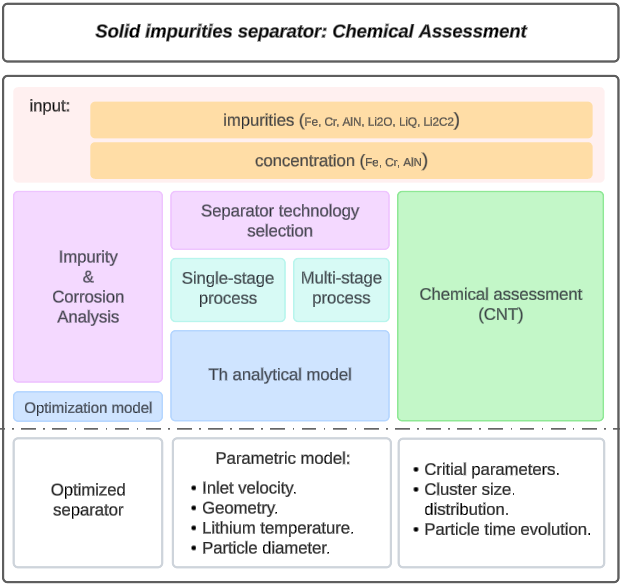
\includegraphics[width=0.8\linewidth]{methodology.png}
	\captionsetup{font=bf, size=small}
	\caption{Methodology}
	\label{methodology}
\end{figure}



\newpage
\section{INPUTS} % ··························································
 To accurately analyze the impact of the impurities from chemical point of view, the following assumptions based on FLF inputhas been considered to target the impurities concentration, as follows:

\begin{tcolorbox}[colback=blue!5!white,colframe=blue!75!black,title=Inputs \& Assumptions]
	The metallic impurities are calculated in the following manner:
	\begin{itemize}
		\item \textbf{135.000 kg/yr} of insoluble metal per year are generated as impurity.
		\item \textbf{8000 hr/yr} of Reactor Chamber (RC) operation.
		\item Assumed concentration:
		\begin{itemize}
			\item 80\% Fe
			\item 10\% Cr
			\item 10\% AlN 
		\end{itemize}
		\item \textbf{1/10 Hz} of Pulsed operation.
		\item \textbf{439.38 Tn} of LL in the loop.
	\end{itemize}
	Impurities mass  produced in 1 pulse in the entire LL loop: \textbf{0.421 Kg}\\
	\underline{Where the concentrations are:}
	\begin{itemize}
		\item Fe $=$ 0.00839 $\text{mol}/m^3$
		\item Cr $=$ 0.00112 $\text{mol}/m^3$
		\item AlN $=$ 0.00142 $\text{mol}/m^3$
	\end{itemize}
	\underline{With an impurities ratio:}
	\begin{itemize}
		\item Li $=$  0.999 e-00
		\item Fe $=$ 1.201 e-07
		\item Cr $=$ 1.613 e-08
		\item AlN $=$ 2.046 e-08
	\end{itemize}
\end{tcolorbox}



\newpage
\section{IMPURITY AND CORROSION ANALYSIS} \label{sec:impurity}% ··························································
\subsection{Impurities Matrix}

Within the scope of the current document, the identification of the impurities source and its main properties is key to provide the necessary context for the coming sections. Given the FLF machines and components, such as: machine gun (upper launcher), Reactor Chamber (RC), and the liquid lithium primary loop, the identified impurity sources are:

\begin{itemize}
	\item \textbf{Lithium initial impurities}.
	\item \textbf{Corrosion:} mainly given by the primary loop (piping and components) made of SS316-Ti, it is assumed at some point the RC vessel made of P91 will be a secondary source of corrosion impurities. The section \ref{sec:corrosion} is dedicated to identify the corrosion products, mechanisms, and its source.
	\item \textbf{Pulsed shot (projectile + target):} considering the input metallic impurities given by FLF (Fe, Cr, AlN), it is assumed in the current document that part of these impurities will be generated at the pulsed operation due to the projectile impact with the target, example of this is the presence of Cr. Future studies will be necessary to identify and classify the impurities result of the pulsed operation. 
\end{itemize}

\subsubsection{Lithium initial impurities}

The initial lithium impurities is a key source in terms of traceability, even more  considering that these impurities can mutate within the system under neutronic irradiation. The Figure \ref{Li_init_imp_chart} shows the list of impurities, ranked in the horizontal axis by concentration and vertically the density of element.  

\begin{figure}[H]
	\centering
	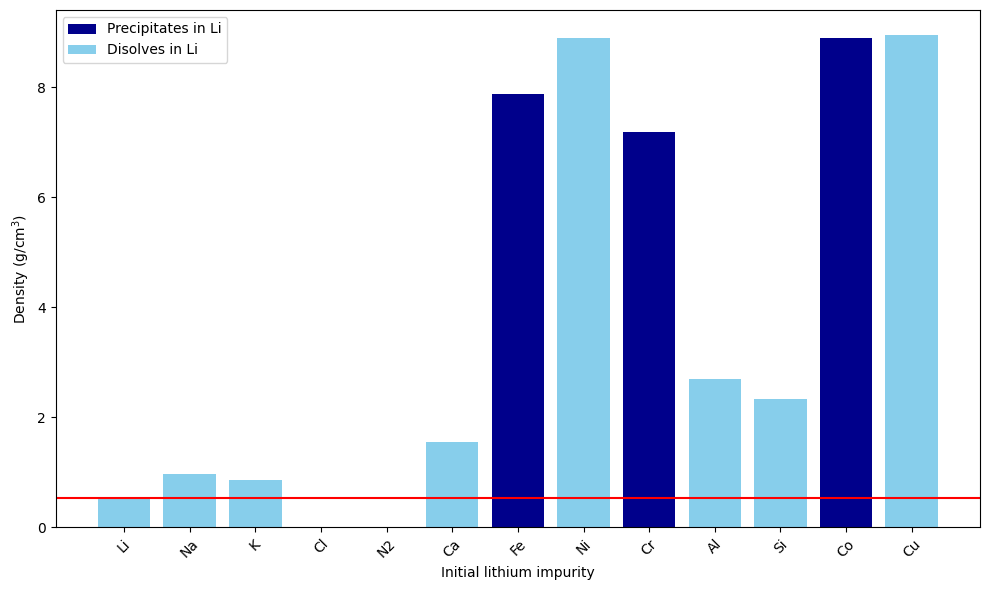
\includegraphics[width=0.97\linewidth]{Li_init_imp_chart.png}
	\captionsetup{font=bf, size=small}
	\caption{Initial lithium impurities.}
	\label{Li_init_imp_chart}
\end{figure}


xxxxxxxxxxxxxxxxxxxxxxxxxxxxxxxxxxxx  explanation here about the results in the graph, 




\begin{table}[H]
	\centering
	\begin{tabular}{ccc}
		\rule[-0.3cm]{0pt}{0.8cm}\textbf{Element}   & \textbf{Content} & \textbf{Density} \\ \Xhline{1.3pt}
		\rule[-0.3cm]{0pt}{0.8cm} Li & 99.98 \% & 0.534 g/cm$^3$ \\ \hline
		\rule[-0.3cm]{0pt}{0.8cm} Na & 0.0034 \% & 0.971 g/cm$^3$ \\ \hline
		\rule[-0.3cm]{0pt}{0.8cm} K & 0.0032 \%  & 0.862 g/cm$^3$ \\ \hline
		\rule[-0.3cm]{0pt}{0.8cm} Cl & 0.0031 \% & 0.003214 g/cm$^3$  \\ \hline
		\rule[-0.3cm]{0pt}{0.8cm} $N_2$ & 0.0020 \% & 0.001250 g/cm$^3$ \\ \hline
		\rule[-0.3cm]{0pt}{0.8cm} Ca & $<$ 0.001 \%  & 1.550 g/cm$^3$ \\ \hline
		\rule[-0.3cm]{0pt}{0.8cm} Fe & $<$ 0.001 \%  & 7.874 g/cm$^3$ \\ \hline
		\rule[-0.3cm]{0pt}{0.8cm} Ni & $<$ 0.001 \%  & 8.900 g/cm$^3$ \\ \hline
		\rule[-0.3cm]{0pt}{0.8cm} Cr & $<$ 0.001 \%  & 7.190 g/cm$^3$ \\ \hline
		\rule[-0.3cm]{0pt}{0.8cm} Al & $<$ 0.001 \%  & 2.702 g/cm$^3$ \\ \hline
		\rule[-0.3cm]{0pt}{0.8cm} Si & $<$ 0.001 \%  & 2.330 g/cm$^3$  \\ \hline
		\rule[-0.3cm]{0pt}{0.8cm} Co & $<$ 0.001 \%  & 8.900 g/cm$^3$ \\ \hline
		\rule[-0.3cm]{0pt}{0.8cm} Cu & $<$ 0.001 \% &  8.960 g/cm$^3$ \\ \hline
	\end{tabular}
	\captionsetup{font=bf, size=small}
	\caption{Lithium initial impurities concentration ref. \cite{Ott1970}.}
	\label{li_imp}
\end{table}








\newpage
\subsection{Corrosion Products}\label{sec:corrosion}
The deliverable \cite{SoA}, listed the lithium impurities and how they are related with the corrosion products together with the effects in steel pipework (SS316). The current section, aims to provide more information gathered form the literature, producing the following table:

\begin{table}[h!]
	%\centering
	\begin{tabular}{p{2cm}p{3cm}p{3.5cm}p{3.5cm}p{2cm}}
		\rule[-0.3cm]{0pt}{0.8cm} \textbf{Li impurities} & \textbf{Effect on Materials} & \textbf{Corrosion Product} & \textbf{Conditions/Notes} & \textbf{References} \\ \hline
		\rule[-0.3cm]{0pt}{0.8cm} Nitrogen & General dissolution and intergranular penetration in stainless steel. & Primary attack via chromium forming Li9CrN5 and iron forming Li3FeN2. & High nitrogen levels lead to corrosion at temperatures between 400-600°C. & \cite{Keough1985}, \cite{Chopra1988}, \cite{Muroga2008}, \cite{Heinzel2006} \\ \hline
		\rule[-0.3cm]{0pt}{0.8cm} Oxygen & Formation and dissolution of unstable ternary oxides. & Li5FeO4, LiCrO2, Li2Ni8O17 formed between Li2O and steels. & Limited information, reactions involve Li2O interacting with Fe, Cr & \cite{IAEA2020}, \cite{Finn1981}, \cite{PULHAM1984} \\ \hline
		\rule[-0.3cm]{0pt}{0.8cm} Carbon & Formation of Cr23C6 precipitates on stainless steel surfaces. & Cr23C6 precipitates enhance chromium concentration at the surface. & Higher weight loss in type 316 stainless steel compared to 9Cr1Mo ferritic steel. & \cite{Parida2019} \\ \hline
		\rule[-0.3cm]{0pt}{0.8cm} Hydrogen & Significant decarburisation of stainless steel. Formation of new phase $Fe_{50}Cr_{43}Mo_{3}Ni_{4}$ on steel surface exposed at 700 $^\circ$C showing intergranular corrosion. & Decrease in carbon content more pronounced in austenitic steel. & Affects both austenitic and ferritic/martensitic steels. & \cite{Parida2019} \cite{Xia2019} \\ \hline
		\rule[-0.3cm]{0pt}{0.8cm} Aluminium & Not known to cause corrosion in stainless steel directly. & Addition of Al reduces weight loss in stainless steel; may form AlN in presence of dissolved nitrogen. & Adding 5wt\% Al to lithium reduced weight loss of type 316 stainless steel. & \cite{Tortorelli1980}, \cite{Keough1985} \\ \hline
		\rule[-0.3cm]{0pt}{0.8cm} No impurities added. & The austenitic area in the welded joint showed morphological changes induced by the dissolution of Ni in Li. The ferritic parts exhibit a fine-grained surface structure. & $M_{23}C_{6}$ and $NiC_x$ particles in sizes of 1-2 $\mu$m. & Study of welded joints (SS316 and SS410) in liquid lithium. & \cite{Xia2019}, \cite{Tsisar2019} \\ \hline
		
	\end{tabular}
	\captionsetup{font=bf, size=small}
	\caption{Corrosion Effects of Impurities in Liquid Lithium on Materials.}
	\label{corrosion_effects}
\end{table}


\newpage
\subsection{Maroni's Process}

The Maroni process has been studied in the SoA deliverable ref. \cite{SoA}, where the process diagram Figure \ref{maroni} of a molten-salt extraction and its stages were analyzed. Nevertheless, the current section is focused in study the advantages/disadvantages of Maroni process, presented in Table \ref{ad_dis_maroni}.  

\begin{figure}[H]
	\centering
	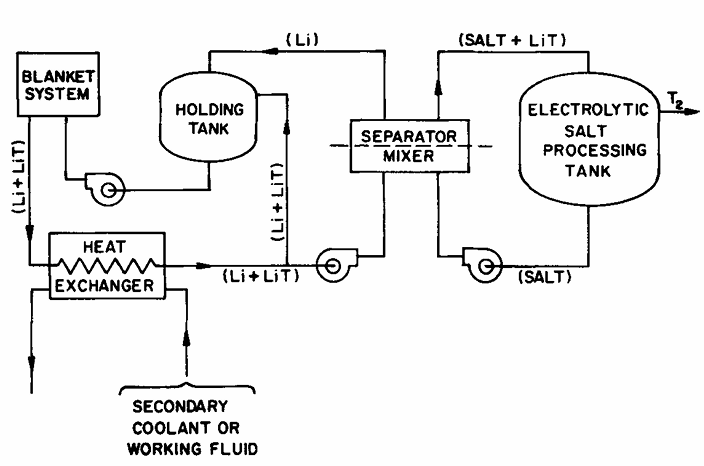
\includegraphics[width=0.7\linewidth]{maroni_schema.png}
	\captionsetup{font=bf, size=small}
	\caption{Schematic diagram of a molten-salt extraction diagram \cite{Maroni1975}.}
	\label{maroni}
\end{figure}

\noindent Before jumping in the Table \ref{ad_dis_maroni}, it is important to remind the Maroni process: based on high temperature molten mixed alkali-metals halide salts (LiCl-KCl at 530 $^\circ$C) as an extraction solvent for the Li + LiT.


\begin{longtable}{p{7.5cm}p{7.5cm}}  
	\rule[-0.3cm]{0pt}{0.8cm} \textbf{Advantages} & \textbf{Disadvantages} \\
	\hline
	\endfirsthead
	
	\rule[-0.3cm]{0pt}{0.8cm} \textbf{Advantages} & \textbf{Disadvantages} \\
	\hline
	\endhead
	
	\endlastfoot
	
	\rule[-0.3cm]{0pt}{0.8cm} \noindent \textbf{Continuous tritium extraction:} The capability to maintain a steady-state tritium inventory within the lithium loop has been incorporated as a critical consideration in the design of the RTPR. This aspect of the design underscores the importance of ensuring a consistent tritium flow and concentration within the system, which is fundamental to the reactor's operational efficiency and safety.  & \textbf{Solubility:} At the operational temperatures of mixing/separating the lithium and salts, the saturation solubility will be reached in the other. The main concern is the presence of salt dissolved in lithium, being significant in terms of corrosion and the products formed under neutronic irradiation (with regard of long-lived radioactive-isotope from the presence of KCl in the lithium jets).  \\
	\hline
	
	
	\rule[-0.3cm]{0pt}{0.8cm} \textbf{Tritium-salts affinity:} The distribution coefficients for 500-600 $^\circ$C are 2.6 for volumetric distribution and 5.8 for molar distribution, being the ratio of tritium content in the salt ($T_{salt}$) to tritium content in lithium ($T_{Li}$) demonstrating that distributions of LiT between the salt and metal phases can be achieved. This advantage of tritium-salts affinity, might allow tritium recovery in the HEX system. & \textbf{Required potential (V):} The extraction of tritium from the salt medium is proposed to be conducted via electrolysis at a potential of 1.5V. However, this process is constrained by the limitation that salt decomposition occurs at potentials exceeding 2.0V. Consequently, to maintain the integrity of the salt medium while ensuring a steady-state tritium inventory, the efficiency of the tritium recovery process must be optimized for operation at the designated 1.5V potential.  \\ \hline
	
	\rule[-0.3cm]{0pt}{0.8cm} \textbf{Density:} Lithium density is less dense than the molten salt by a factor or 3, thus leading to exploit separation system from gravitational settling to centrifugal action. The later separation system could be exploited with hydrocyclones due to its efficiency and low energy cost. & \textbf{Corrosion:} The interaction of materials with lithium, particularly in contexts requiring controlled corrosion rates, remains a significant area of ongoing research. This challenge is further intense in scenarios involving lithium-salt mixtures within mixing/separator devices. To mitigate these issues, the employment of specialized alloys, such as Niobium, was studied in the literature. However, the selection of appropriate materials for lithium loops presents complex considerations, notably due to the specific corrosion behaviors and operational temperature demands associated with fusion nuclear environments. \\ \hline
	
	\rule[-0.3cm]{0pt}{0.8cm}  & \textbf{Volatile elements:} The use of electrolytic process to extract the tritium from salts could involve potential volatile elements such as hydrogen chloride, hydrogen fluoride, hydrogen bromide or its tritium analogs have a direct impact in the feasibility of the tritium extraction in form of gas. Recent studies mitigate the volatile using benign lithium hydroxide (LiOH) or lithium carbonate (Li$_2$CO$_3$).  \\ \hline
	\captionsetup{font=bf, size=small}
	\caption{Maroni process: advantages/disadvantages \cite{Maroni1975}, \cite{Bandhauer2013}.}
	\label{ad_dis_maroni}
\end{longtable}

\newpage
\section{CHEMICAL ANALYSIS} \label{sec:chem}% ··························································

This section investigates the nucleation of impurities within liquid lithium, which serves as a breeder and shielding material in the reaction chamber. The nucleation of impurities within liquid lithium poses a 
complex challenge, impacting not only the material's thermal and physical properties but also the safety and longevity of the fusion reactors. Despite its significance, 
the study of impurity nucleation in liquid lithium remains underexplored, with limited literature providing a comprehensive understanding of these mechanisms.
\\
Due to the objective of using purification processes based on centrifugation phenomena, the limiting factor of these impurities will be their densities, the quantities in which 
they are present and above all the particle size of these impurities. Therefore, as a starting point for the characterisation of these impurities from a thermodynamic and kinetic point of view, 
classical nucleation theory (CNT) and kinetic theory have been used to study the evolution and speed of this phenomenon.
\\
The primary issue with this model stems from its oversimplifications, which will be detailed in subsequent sections. A significant limitation is that these models originate from statistical mechanics, 
constraining them to a limited number of particles. Specifically, when examining clusters of macroscopic particles on the scale of micrometers, employing statistical mechanics or molecular dynamics models proves 
impractical. Consequently, for such scales, the application of continuous models becomes more appropriate, examples of which include phase field models \cite{Zhu2004,Garcia}, computational fluid dynamics or precipitation dynamics \cite{Sommitsch}.

Furthermore, this research can serve as a foundational basis for applying continuous models more effectively. For instance, one could enhance these models by incorporating the distributions of nanometric particles within the system as input parameters. 
\\
This section is structured for clarity and comprehension, starting with an explanation of classical nucleation theory and the thermodynamics of the nucleation process. This is followed by an analysis 
of the kinetic treatment of the process. 
The section concludes with the characterization of each impurity.

\subsection{Nucleation Theory}
First-order phase transitions, such as the condensation of vapor, boiling of a liquid, and crystallization of a melt, are critical phenomena in materials science and thermodynamics.
The decay of metastable states, such as the solidification of a supercooled liquid, takes place through the nucleation and growth of some small-sized clusters within the system \cite{Larissa}. The 
initial stage of the phase transformation is usually described within the time-honored CNT \cite{Volmer1926,Hayashi1974}, where the droplet is described as a sphere of, say, bulk solid, 
separated from the liquid by a sharp interface, giving rise to a free-energy penalty proportional to the interface area and a total Gibbs-free-energy activation barrier.

\begin{equation}
    \Delta G(i) = -|\Delta\mu|i + A\gamma_{\infty} i^{2/3},
\end{equation}

where \(i\) is the number of particles in the cluster, \(\Delta\mu < 0\) is the chemical potential difference between the two phases, \(A = (36 \pi \nu^2)^{1/3}\) being \(\nu\) 
the molecular volume and \(\gamma_{\infty}\) the specific surface energy (surface tension) of the planar interface, all anisotropies being neglected at this stage. The droplet grows if it exceeds a 
critical size \(i^\ast\) corresponding to the maximum \(\Delta G(i)\) (\(\equiv \Delta G^\ast\)). 
The CNT relies on the liquid droplet model, which assumes that tiny droplets possess the same characteristics as the bulk 
condensed phases and have surface energies identical to those of an infinite flat surface. Nonetheless, there is an ongoing 
debate about the applicability of macroscopic thermodynamic principles to describe liquid drops when dealing with small clusters 
composed of merely a few dozen molecules \cite{Wilemski}. The inadequacy of the droplet model for small particles is highlighted by the fact that the 
energy required to form monomers is not zero \cite{Gránásy}. This indicates that the attributes of small clusters cannot be 
simply categorized into bulk and surface properties, rendering the notion of surface tension somewhat misleading when applied to these clusters \cite{Anisimov}.
For instance, the 'monomers' of the new phase are indistinguishable from the molecules of the parent phase, leading to the conclusion that the free energy of monomers should logically 
be zero (\(\Delta G(1) = 0\)) \cite{Laszlo1}. 
\\
However, in the conceptual state of this work, this simple model is useful to provide quantitatively and qualitatively the critical size of these nuclei.
\\
CNT also is able to estimate the nucleation rate

\begin{equation}
    I = I_0 e^{-\beta \Delta G^\ast},
\end{equation}

where \(\beta = 1/(k_B T)\) is the inverse temperature and \(I_0\) a kinetic prefactor that varies slowly with \(T\). Clearly, this connection between \(I\) and \(\gamma_{\infty}\) relies 
on several severe approximations. Moreover, \(I_0\) is notoriously influenced by genuinely non-equilibrium effects and various expressions resulting from a more detailed consideration of the nucleation kinetics are known since a 
long time \cite{Hayashi1974}.

\paragraph{} In the nucleation regime, the evolution of the system is significantly marked by the formation of clusters that represent a new equilibrium phase. The dynamics of this process 
are intricately governed by the balance between volume and surface contributions, as encapsulated by the capillary approximation. The volume contribution, acting as the driving 
force behind nucleation, lowers the system's free energy and is directly proportional to the cluster's volume, thereby favoring the formation and growth of these clusters. Conversely, 
the surface contribution introduces an energetic cost, scaling with the cluster's surface area. This cost is associated with creating an interface between the original phase and the new 
cluster, serving as a barrier that inherently inhibits the growth of the cluster \cite{Clouet1}.

The critical size of the nucleus and the nucleation barrier are determined by setting the derivative of \(\Delta G\) with respect to the size, \(i\), equal to zero:

\begin{equation}
    R^* = -2\gamma_{\infty} (\Delta \mu / \nu)^{-1},
\end{equation}

and

\begin{equation}
    \Delta G^\ast = \frac{16 \pi}{3} \gamma_{\infty}^3(\Delta \mu / \nu)^{-2}.
\end{equation}

Analyzing the critical parameters obtained from the CNT, is it evident that the key variables of the model are the nucleation driving force and the surface energy. In the following sections,
some formalisms for the driving force will be presented and discussed, as well as for the surface energy. 
\subsubsection{Driving force}
The nucleation driving force is obtained by considering the difference in chemical potentials between the parent and the equilibrium phases for all atoms composing the cluster:

\begin{equation}
    \Delta \mu = \sum_i y_i^e (\mu_i^e - \mu_i^0),
\end{equation}

where \(y_i^e\) is the atomic fraction of type \(i\) atoms in the nucleating equilibrium phase, and \(\mu_i^e\) and \(\mu_i^0\) are the corresponding chemical 
potentials in the nucleating equilibrium phase and in the parent phase, respectively. In a metastable parent phase, chemical potentials are higher than those at equilibrium. 
The critical factors for applying CNT are the driving force, \(\Delta \mu\), and the surface energy, \(\gamma_{\infty}\), of the solid particle. The driving force depends 
on the nucleation pathway, such as the saturation-based formalism commonly used in the context of vapor to liquid or crystal transitions \cite{Myerson2019, Ford2004, Sun2009}:

\begin{equation}
    \Delta\mu = \mu - \mu_{\text{coex}} = kT \ln\left(\frac{n_1}{n_1^{\text{sat}}}\right),
\end{equation}

where the chemical potential is represented using the ideal gas expression, introducing a monomer density \(n_1^{\text{sat}}(T)\) appropriate to a saturated vapor, i.e., a gas phase in coexistence with the condensed phase at the environmental temperature. The ratio of the monomer density in a metastable vapor to its value in a saturated vapor defines the supersaturation, \(S\):

\begin{equation}
    \Delta\mu = kT \ln S.
\end{equation}

This driving force dictates the nucleation process, which is governed by temperature, the degree of supersaturation, and the interfacial energy. The nucleation rate increases with the degree of supersaturation and temperature and decreases with the interfacial energy. This behavior is illustrated in Figure \ref{fig:free_energy_illustrative_degree_saturation}, which shows the energy barrier that must be overcome to form a new phase for various degrees of supersaturation.

\begin{figure}[H]
    \centering
    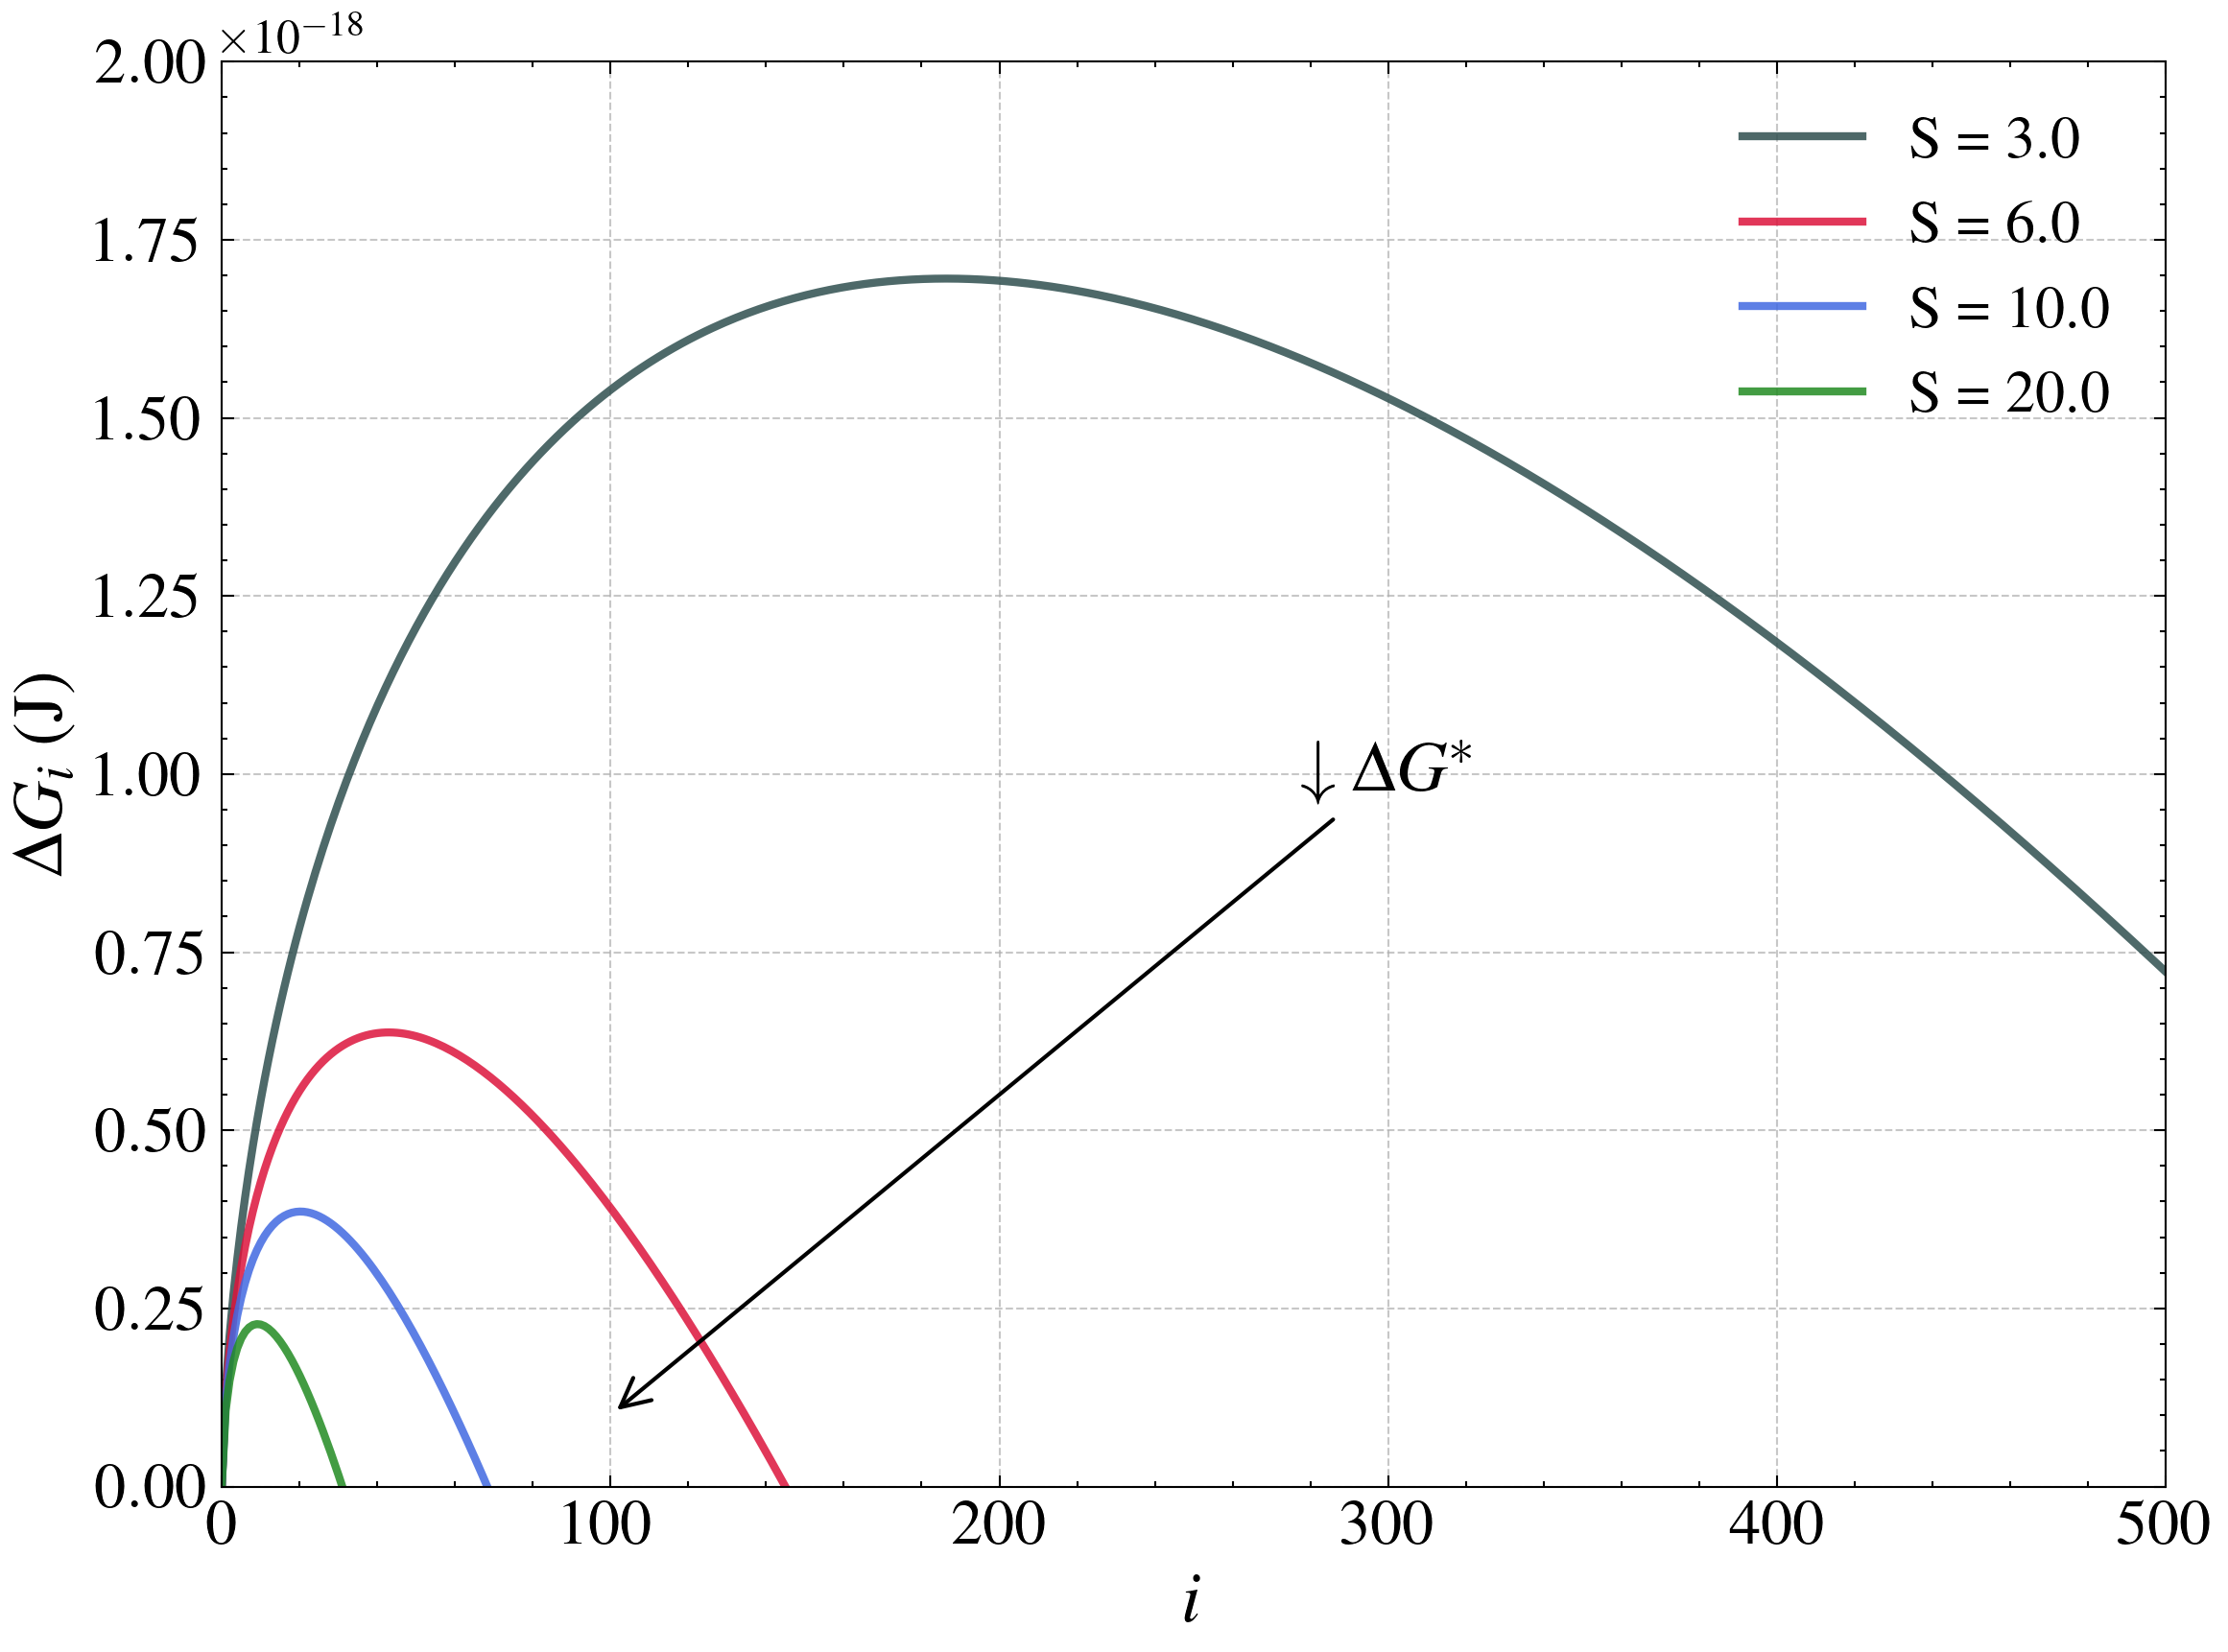
\includegraphics[width=0.9\linewidth]{free_energy_illustrative_degree_saturation.png}
    \caption{Required free energy, as per classical nucleation theory, for the formation of a cluster of size \(i\). Curves represent different constant values of supersaturation and temperature, illustrating the free energy barrier associated with the critical size.}
    \label{fig:free_energy_illustrative_degree_saturation}
\end{figure}

This formalism is pertinent for analyzing solutes dissolved in liquids that nucleate in either liquid or crystalline states. However, CNT is not 
always successful, primarily because the capillarity approximation, upon which it is based, is a very primitive characterization of small molecular clusters. 
Nevertheless, the expressions derived provide intuitive value, suggesting that increasing the vapor supersaturation, \(S\), accelerates the nucleation of droplets, 
all other parameters being constant. Additionally, the nucleation rate is influenced by the surface tension of the condensed phase: higher surface 
tension, \(\gamma_{\infty}\), results in a slower rate. The rate is also quite sensitive to supersaturation, surface tension, and temperature, as 
these quantities appear inside an exponential function \cite{Ford}.

To surpass the predictive capability of classical theory, it is necessary to compute the partition functions of clusters of various sizes and develop 
a more realistic model of the excess free energy; however, this is beyond the scope of this work.

Another formalism that may be useful for this study involves the definition of the driving force commonly used in the phase transition between melts 
and crystalline phases. Consider a single-component liquid initially at equilibrium, quenched to a temperature \(T\), below its melting 
temperature \(T_m\). Since the liquid and solid phases have the same composition, the nucleation free energy corresponds to the free 
energy difference between the liquid and solid states at temperature \(T\), in other words, the driving force is a function that depends 
on the undercooling rate \cite{Clouet1, Fokin2006}:

\begin{equation}
    \Delta\mu = \frac{\Delta H_{m}}{T_{m}}(T_{m} - T) + \int_{T}^{T_{m}} \Delta C_{p} dT' - T \int_{T}^{T_{m}} \frac{\Delta C_{p}}{T'} dT',
\end{equation}

where \(\Delta H_{m}\) and \(T_{m}\) are the molar heat of melting and the melting temperature of the crystal, respectively, and \(\Delta C_{p} = C_{p}^{l} - C_{p}^{c}\) is the difference between the molar heat capacities of liquid and crystal at constant pressure. The experimental values of \(\Delta G_{V}\) are normally bounded by the approximations usually assigned to Turnbull and Hoffman that assume \(\Delta C_{p} = 0\) and \(\Delta C_{p} = \) constant, respectively:

\begin{equation}
    \Delta\mu(T) =  \frac{\Delta H_{m}}{N_A} \left( 1 - \frac{T}{T_{m}} \right),
	\label{fig:turnbull_delta}
\end{equation}

\begin{equation}
    \Delta\mu(T) = \frac{\Delta H_{m}}{N_A} \left( 1 - \frac{T}{T_{m}} \right) \frac{T}{T_{m}},
	\label{fig:hoffmann_delta}
\end{equation}

Here, \(\Delta H_{m}\) is the melting enthalpy per mole of the crystal and \(N_A\) is Avogadro's number. When the undercooling is large, the expression may not be precise enough. One can then consider the next term in the Taylor expansion leading to the Turnbull and Hoffman equations respectively \cite{Clouet1}:

\begin{equation}
    \Delta\mu(T) = \frac{\Delta H_{m}}{N_A} \left( 1 - \frac{T}{T_{m}} \right)  - \Delta C_{p} \left( \frac{(T - T_{m})^2}{2T_{m}} \right),
\end{equation}

\begin{equation}
    \Delta\mu(T) =  \frac{\Delta H_{m}}{N_A} \left( 1 - \frac{T}{T_{m}} \right) \frac{T}{T_{m}}   - \Delta C_{p} \left( \frac{(T - T_{m})^2}{2T_{m}} \right).
\end{equation}

This formalism is widely used in the study of the nucleation of impurities in metallic melts, with a wide range of materials, such 
as metallic glasses like Li\(_2\)O\(_2\)SiO\(_2\) and LS\(_2\), or other metallic alloys 
like Ge\(_2\)Sb\(_2\)Te\(_5\) and (Ag,In)-doped Sb\(_2\)Te (AIST) \cite{Laszlo1, Neilson1979, Kelton1983, Laszlo3, Laszlo4, Sun2009}.

Using these models to describe the driving force, they exhibit certain limitations. Firstly, within the 
formalism derived from the degree of saturation, an ideal mixture is assumed. This is evident since 
concentrations or mole fractions are used to determine the degree of supersaturation rather than activities. 
To rigorously work through activities, the driving force can be determined if the interaction parameters 
between the components of the solution are known \cite{Bartels1991}, or determine the mixing parameters 
starting from the partition function derived from the grand canonical potential, employing the quasi-chemical approximation formulation \cite{Odusote2020} or 
exponential models \cite{Yadav2023}.

In the second formulation, which utilizes the undercooling rate to determine the driving force, the approach is widely 
recognized and accepted. However, this formula encounters limitations when applied to mixtures exhibiting degrees of immiscibility. 
Specifically, the challenge arises in scenarios where two phases coexist, such as in solid-liquid equilibrium. In these instances, 
given a particular composition for which a certain temperature allows both phases to be in equilibrium; this temperature is referred 
to as the liquidus temperature \(T_l\).

The standard application of this formulation presents issues as it traditionally employs the absolute melting point to determine the 
driving force, neglecting the presence of different phases that may manifest within the system.

A potential rectification for this oversight involves the utilization of the \(T_l\) instead of \(T_m\). However, this correction 
is not without its challenges. Specifically, when the fraction of one of the phases is exceedingly low, accurately determining the 
liquidus temperature within the phase diagram becomes problematic. This difficulty is compounded by the typical unavailability of high-resolution phase diagrams.


Ideally, the driving force in phase transition studies is determined by a comprehensive thermodynamic model that includes 
information about the elements present in the system, as demonstrated in previous works \cite{Was1985, Kumar1996}. However, 
due to the limitations previously stated, an alternative formulation for the driving force has been developed to provide a more 
accurate description of the volumetric free energy. This method involves calculating the Gibbs free energy change, \(\Delta G\), 
defined by the free energy expressions for the liquid (\(l\)) and solid (\(s\)) phases.

The chemical potential for component A in the liquid phase, \(\mu_A^l\), is determined by constructing a tangent to the liquid 
free energy curve at the composition \(x_l\). The point where this tangent line intersects the \(x_A = 1\) axis defines \(\mu_A^l\). 
Similarly, the chemical potential for component A in the solid phase, \(\mu_A^s\), is identified at the intersection of the tangent line with the \(x_A = 0\) axis.

At the liquidus temperature \(T_l\), the free energy curves for both the liquid and solid phases are tangent to the line constructed 
from the previous step. The solid composition that is in equilibrium with the liquid composition \(x_l\) at \(T_l\) is given by the 
tangent point on the Gibbs free energy curve. This equilibrium composition is denoted as \(x_{s,eq}\) and can be identified on the equilibrium phase diagram.

At a temperature \(T\), arbitrarily lower than \(T_l\), the chemical potentials in the solid, \(\mu_A^s\) and \(\mu_B^s\), and for 
the liquid, \(\mu_A^l\) and \(\mu_B^l\), are determined as before for the liquid phase. The differences in chemical potential, which 
drive the phase transition, are defined as follows:

\begin{equation}
\Delta\mu_A = \mu_A^l - \mu_A^s \label{eq:delta_mu_A}
\end{equation} 

\begin{equation}
\Delta\mu_B = \mu_B^l - \mu_B^s. \label{eq:delta_mu_B}
\end{equation} 

The free energy change, per unit volume, associated with forming a small amount of solid of composition \(x_{s}^\ast\) out of the liquid is given by
\begin{equation}
\Delta G_v = [x_s^A \Delta\mu_A + (1 - x_s^A) \Delta\mu_B]/V \label{eq:delta_G_v}
\end{equation} 

where \(V\) is the average molar volume of the solid, assumed here to vary linearly between the molar volumes \(V^A\) and \(V^B\) of the pure solid systems:
\begin{equation}
V = x_s^A V^A + (1 - x_s^A) V^B. \label{eq:V}
\end{equation}
The solid composition that is most likely to nucleate, \(x_n\), is assumed to be the one with the largest difference in free energy, \(\Delta G_v\), between the liquid and solid state. This intuitively obvious assumption is used because of its simplicity. Further justification based on a more rigorous calculation is given in Appendix I. It can be seen from that \(\Delta G_n\) is maximized if \(\Delta \mu^A = \Delta \mu^B\), so that the composition \(x_n\) corresponds to the point of tangency on the solid curve of a line parallel to the tangent to the liquid curve at \(x_l\), so that
\begin{equation}
\bar{\Delta G_v} \approx \Delta \mu^A \approx \Delta \mu^B. \label{eq:bar_delta_G_v}
\end{equation}
Therefore, given the composition dependence of the liquid and solid free energies, one can calculate the solid nucleus composition and the free energy of formation for the nucleus as a function of initial liquid composition, \(x_l\), and undercooling \(\Delta T = T_l - T\).

For an actual calculation of \(\Delta G_p\), it is necessary to use solution models. Therefore, regular solution behavior is assumed for the liquid phase so that
\begin{align}
\mu_l^A &= \mu_l^{A,0} + RT \ln(x_l^A) + \alpha_l(x_l^A), \label{eq:mu_l_A} \\
\mu_l^B &= \mu_l^{B,0} + RT \ln(x_l^B) + \alpha_l(x_l^B). \label{eq:mu_l_B}
\end{align}

The solid phase is assumed to be a dilute or ideal solution so that \(\alpha_s^A\) and \(\alpha_s^B\) are independent of composition:

\begin{align}
\mu_s^A &= \mu_s^{A,0} + RT \ln(x_s^A) + \alpha_s^A, \label{eq:mu_s_A} \\
\mu_s^B &= \mu_s^{B,0} + RT \ln(x_s^B) + \alpha_s^B. \label{eq:mu_s_B}
\end{align}

Combining equations \eqref{eq:mu_l_A} and \eqref{eq:mu_s_A} gives

\begin{equation}
\Delta \mu^A = (\mu_l^{A} - \mu_s^{A}) + RT \ln\left(\frac{x_l^A}{x_s^A}\right) + \alpha_l(x_l^A) - \alpha_s^A. \label{eq:delta_mu_A_solution}
\end{equation}

For pure metals, it can be assumed that the difference between the heat capacities of the solid and liquid, \(\Delta C_p\), is small, so that

\begin{equation}
\mu_l^{A,0} - \mu_s^{A,0} \approx \Delta S_f (T_m^A - T), \label{eq:mu_difference_pure_metals}
\end{equation}

where \(\Delta S_f\) and \(T_m^A\) are, respectively, the entropy of fusion and the melting temperature of pure A. Therefore, combining equations \eqref{eq:delta_mu_A_solution} and \eqref{eq:mu_difference_pure_metals} gives

\begin{equation}
\Delta \mu^A = T \left[ R \ln\left(\frac{x_l^A}{x_s^A}\right) - \Delta S_f \right] + \alpha_l'(x_l^A), \label{eq:combined_delta_mu_A}
\end{equation}

where
\begin{equation}
\alpha_l'(x_l^A) = \alpha_l(x_l^A) - \alpha_s^A + \Delta H_f. \label{eq:alpha_prime_A}
\end{equation}

Similarly, for component B
\begin{equation}
\Delta \mu^B = T \left[ R \ln\left(\frac{x_l^B}{x_s^B}\right) - \Delta S_f \right] + \alpha_l'(x_l^B). \label{eq:delta_mu_B_solution}
\end{equation}

Now recall that at \(T = T_l\), \(\Delta \mu^A = 0\) so that
\begin{equation}
\alpha'(x_l^A) = -T_l \left[ R \ln\left(\frac{x_l^A}{x_{s,eq}^A}\right) - \Delta S_f^A \right]. \label{eq:alpha_prime_equilibrium_A}
\end{equation}
For a given \(x_l^A\), \(T_l\), and \(x_{s,eq}^A\) can be found from the equilibrium phase diagram. Combining equations \eqref{eq:combined_delta_mu_A} and \eqref{eq:alpha_prime_equilibrium_A} and rearranging terms gives
\begin{equation}
\Delta \mu^A = (T_l - T) \Delta S_f^A + RT \ln\left(\frac{x_l^A}{x_{s}^A}\right) - RT_l \ln\left(\frac{x_l^A}{x_{s,eq}^A}\right). \label{eq:final_delta_mu_A}
\end{equation}
Similarly, for component B
\begin{equation}
\Delta \mu^B = (T_l - T) \Delta S_f^B + RT \ln\left(\frac{x_l^B}{x_{s}^B}\right) - RT_l \ln\left(\frac{x_l^B}{x_{s,eq}^B}\right). \label{eq:final_delta_mu_B}
\end{equation}
Finally, as discussed previously, at \(T < T_l\), the free energy change on nucleation is
\begin{equation}
V \Delta G_v = \Delta \mu^A = \Delta \mu^B. \label{eq:free_energy_change_nucleation}
\end{equation}
Also, since \(\Delta \mu^A = \Delta \mu^B\), from equations \eqref{eq:final_delta_mu_A} and \eqref{eq:final_delta_mu_B}
\begin{equation}
(T_l - T)(\Delta S_f^A - \Delta S_f^B) + RT \ln\left(\frac{x_l^A(1 - x_{s}^A)}{x_{s,eq}^A(1 - x_l^A)}\right) = RT \ln\left(\frac{x_l^A(1 - x_{s,eq}^A)}{x_{s,eq}^A(1 - x_l^A)}\right). \label{eq:final_energy_balance}
\end{equation}

Therefore, given \(x_l\), \(\Delta S_f^A\), \(\Delta S_f^B\), and the equilibrium phase diagram, one can find \(\Delta G\), and \(x_n\) at an arbitrary temperature \(T\) from equations \eqref{eq:final_delta_mu_A}--\eqref{eq:final_energy_balance}. In the limiting case that the solubility of B in crystalline A is zero, the derivation simplifies considerably. Equation \eqref{eq:mu_l_A} still holds but equation \eqref{eq:mu_s_A} becomes \(\mu_s^A = \mu_{s,0}^A\). Therefore, as before
\begin{equation}
\Delta \mu^A = T(R \ln x_l^A - \Delta S_f^A) + \alpha'(x_l^A) \label{eq:simplified_delta_mu_A}
\end{equation}
and since \(\Delta \mu^A = 0\), at \(T_l\),
\begin{equation}
\alpha'(x_l^A) = -T_l(R \ln x_l^A - \Delta S_f^A) \label{eq:simplified_alpha_prime_A}
\end{equation}
so that
\begin{equation}
V \Delta G_v = \Delta \mu^A = (T_l - T)(\Delta S_f^A - R \ln x_l^A). \label{eq:simplified_free_energy_change}
\end{equation}
An analogous equation holds for crystallization of pure B. This simplified result is particularly useful for metal-metalloid glass forming alloys such as Au–Si where the equilibrium 
solid solubility of the metalloid in the crystalline metal is very low.

\subsubsection{Surface energy}

As discussed in the previous section, surface energy is one of the critical parameters in CNT. Firstly, because this theory fails to predict the behaviour of small clusters 
and at the same time assumes a surface energy value for a flat surface. In addition, the dependence of the surface energy on the nucleation rate is probably the most important part of this formalism. 

Because this parameter is an exponential in the calculation of the nucleation rate, it depends very strongly on the value of the surface tension. For example, a change in $\gamma_{\infty}$ of only one order of magnitude
leads to a change in the nucleation rate of about eight orders of magnitude \cite{Ulbricht1998}.
\\
Nonetheless, a dependable method for measuring surface tension is absent, with the exception of aligning experimental nucleation rate data with theoretical models \cite{Fokin2006HomogeneousCN}. 
Furthermore, a critical hypothesis of the CNT, referred to as the capillarity approximation, overlooks the influence of curvature and size on surface tension \cite{SANGWAL19963}.
Therefore, ideally it has to be obtained from experiments or from ab-initio calculations \cite{Sun2020, Lee2018, Vitos1998, Holec2012, Binnie2010}. 
Another well-accepted methodology is from the complete thermodynamic model of the mixture, using Buttler's formulation \cite{Silva, Picha2004, Krasin2015}, 
the problem with this methodology arises in having all the information and having a detailed phase diagram.
\\
Given the difficulties noted above in measuring or simulating the surface free energy of the liquid-solid interface, the natural question is whether theoretical methods 
can predict its magnitude and the physical processes that affect it. 
theoretical methods can predict its magnitude and the physical processes that affect it. 

In order to determine $\gamma$, it is useful to discuss the energetic and entropic components that make it up, 
since, as we shall see, the different models that have been developed differ markedly in the relative contributions they attribute to these two components. 
The surface Gibbs free energy can be written as
\begin{equation} \label{eq:Gibbs_free_energy}
\gamma = E^{(s)} - T S^{(s)} + P V^{(s)}
\end{equation}
In this context, $E^{(s)}$ represents the energy excess at the surface, $S^{(s)}$ denotes the entropy at the surface, and $V^{(s)}$ is the additional volume. 
The latter term remains negligible unless under conditions of high pressure, and can be completely negated by appropriately selecting the Gibbs dividing surface such 
that $V^{(s)}$ becomes zero. This results in only energetic and entropic elements contributing to $\gamma$.

An early and widely adopted model for assessing the free energy at the liquid-solid interface was introduced by \cite{Skapski1956ATO}. This model 
presupposes complete wetting of the crystal by the liquid, leading to a contact angle $\theta$ of zero in the equilibrium involving three phases: 
crystal, liquid, and vapor. Following from Eq.~\ref{eq:Gibbs_free_energy}, with $\theta$ set to zero and consequently $\cos \theta$ equal to one, the derived expression is
\begin{equation} \label{eq:Skapski_model}
\gamma_{sl} = \gamma_{sv} - \gamma_{lv}
\end{equation}

Assuming the general case holds, the analysis simplifies to evaluating $\gamma_{sv}$ and $\gamma_{lv}$ independently. This method involves deducing the 
energy difference due to bond disruption between the solid-vapor and liquid-vapor phases, incorporating the solid's fusion enthalpy and melting-induced volume 
change, alongside a modest entropic variation from the external layers of both phases. Consequently, the derived formula is
\begin{equation} \label{eq:Skapski_result}
\gamma_{sl} = \frac{\Delta H}{4f N_{A} v^{2/3}} + \frac{2\Delta V}{3V_{s}} \gamma_{lv} + \frac{T_m (\Delta S_l - \Delta S_s)}{f N_{A} v^{2/3}}
\end{equation}
where $f$ is a factor that relates the area $A$ of a mole of surface atoms to the volume of a mole of atoms in the bulk solid through
\begin{equation} \label{eq:relation_factor}
A = f N_{A} v^{2/3}
\end{equation}
Numerically, the factor stands at 1.12 for the bcc (110) surface and 1.09 for the fcc (111) surface. Given the 
minimal entropic contribution in Eq.~\ref{eq:Skapski_model}, this framework primarily emphasizes energy aspects. 
Predominantly, the initial term, hinting at a direct relationship between $\gamma_{sl}$ and $\Delta H/v^{2/3}$, 
aligns with empirical findings from initial nucleation studies, underpinning classical homogeneous nucleation theory.

In \cite{Zadumkin1966SurfaceEA} introduced an energy-centric model for surface free energy, emphasizing electron-ion interactions and 
significant volume changes upon melting. Conversely, Turnbull proposed an entropy-focused model, envisioning the solid as a plane 
intersecting the liquid. 
\begin{equation} \label{eq:Turnbull_model}
\gamma_{sl} = \frac{T_m \Delta S}{2f N_{A} v^{2/3}} - \frac{\Delta H}{2f N_{A} v^{2/3}}
\end{equation}

More recent approaches have applied physical or computational simulations, notably using hard sphere packings, to gauge surface free energy, 
as detailed by \cite{Spaepen1975ASM}. In these models, spheres form a densely packed crystalline structure, excluding octahedral voids 
to mirror the dense liquid's random packing. Preference is given to tetrahedral gaps, aiming to enhance interfacial layer density. After 
assessing the configurational entropy across different surface arrangements, findings indicated no significant density reduction at the 
interface compared to the dense, random liquid structure. This suggests a minimal energetic impact if hard spheres mimic atoms with attractive forces, 
thus classifying the model as predominantly entropic and forecasting minor energy contributions to $\gamma_{sl}$.

\begin{equation} \label{eq:Spaepen_model}
\gamma = \frac{\alpha_m \Delta S_f}{N_{A} v^{2/3}} T
\end{equation}
where $\alpha_m$ is 0.86 for the fcc (111) or hcp (0001) surfaces, and 0.71 for the bcc (110) surface. At $T = T_m$, this has the same form as 
the empirical equation with $\gamma$ proportional to $\Delta H/v^{2/3}$.

Up to now we discussed almost exclusively the case of one-component substances. There is considerable interest, 
in the nucleation of binary mixtures or alloys. Calculations in this case 
require a knowledge of the bulk thermodynamics of the mixtures (both liquid and solid).

In \cite{Thompson1983HomogeneousCN} extended the theory of \cite{Spaepen1975ASM} to binary alloys. They use Eq.~\ref{eq:Spaepen_model}

\begin{equation} \label{eq:Thompson_Spaepen_model}
\gamma = \frac{\alpha_m \Delta S_f}{N_{A} v^{2/3}} T
\end{equation}
and take $v$ to change linearly with mole fraction between its values for the two pure components. In the same way they take
\begin{equation} \label{eq:Delta_S}
\Delta S_f = x_s^A \Delta S_f^A + (1 - x_s^A) \Delta S_f^B
\end{equation}
where $x_s^A$ is the mole fraction of A in the solid and $\Delta S_f^A$ and $\Delta S_f^B$ are the entropies of fusion of the two separate components.

This last equation is simple and useful as a starting point to obtain the surface energy for each impurity.

\subsection{Kinetic theory}
Understanding the nucleation rate necessitates analyzing the dynamics of cluster size evolution. This is addressed 
within the framework of the classical nucleation theory, also identified as the phenomenological or Becker-Döring-Zeldovich (BDZ) theory, 
which is used to our analysis. Define \( N_n(t) \) as the average quantity of clusters containing \( i \) molecules at an instance \( t \). 
It is assumed that the interaction between clusters are neglected. As a result, alterations in the size of the clusters are only 
attributed to the mechanisms of evaporation and condensation, signifying that a cluster containing \( i \) molecules may either enlarge by acquiring another 
molecule or diminish through the release of one. Such is the fundamental postulate of the classical nucleation theory. Consequently, the variation in the 
count of clusters of a particular size is governed by what is known as the master equation \cite{Larissa}.

\begin{equation}
\frac{\partial N_i(t)}{\partial t} = J_{i} - J_{i-1},
\label{eq:master_equation}
\end{equation}

where
\begin{equation}
J_i = g^+_{i+1} N_{i+1}(t) - g^-_i N_i(t)
\label{eq:current_size_space}
\end{equation}

is a current in a size space, i.e., it is the rate at which clusters of size \( i-1 \) grow to clusters of 
size \( i \). Here \( g^+_{i+1} \) is the rate of the molecule attachment to a cluster of size \( i \), and \( g^-_i \) 
is the rate of detachment. According to the theory of thermodynamic fluctuations, the equilibrium distribution of clusters obeys the Boltzmann (or Gibbs) distribution
\begin{equation}
N^{\text{eq}}_i = N_0 \exp \left( -\frac{\Delta G_i}{k_B T} \right),
\label{eq:boltzmann_distribution}
\end{equation}

where \(\Delta G_i\) is the minimum work needed to form a cluster of size \(i\), \(k_B\) is Boltzmann’s 
constant, \(T\) is the temperature, and \(N_0\) is a pre-exponential factor.

At equilibrium the current \(J_i\) is zero, as this consequence only the forward rate needs to be specified to calculate the opposte rate.

\begin{equation}
g^+_{i+1} N^{\text{eq}}_{i+1}(t) - g^-_i N^{\text{eq}}_i(t) = 0
\label{eq:current_equilibrium}
\end{equation}

For crystal nucleation in melt or glass, the rate of attachment can be expressed as
\begin{equation}
g^+_{n-1} = bD \lambda^{-2/3} i^{-2/3} \exp\left(-\frac{\Delta G_{i+1} - \Delta G_i}{2kT}\right),
\label{eq:attachment_rate}
\end{equation}

where \( b = 24 \) is a geometrical factor, \( D \) the diffusion coefficient, and \( \lambda \) the jump distance in the parent phase.
The quantities we are mainly concerned with are the net formation rate of clusters of given size (observable size), and the number density 
of such clusters that exceed this size. The former can be expressed as
\begin{equation}
J_{i_0} = A_{i_0} N_{i_0} - D_{i_0 + 1} N_{i_0 + 1},
\end{equation}
where \( i_0 \) is the number of molecules in the cluster of ``observable'' size, while the latter is given by
\begin{equation}
N_{> i_0} = \sum_{i=i_0}^{\infty} N_i.
\end{equation}
Owing to the finite maximum size one is able to handle in the computations, the evaluation of \( N_{> i_0} \), is not without difficulties, 
and depends on the choice of the boundary conditions.

We set the following initial and boundary conditions. At \( t = 0 \), the cluster distribution is defined 
as \( N_i = N_{\text{eq}, i} \) for \( i < u \), and \( N_i = 0 \) for \( i \geq u \), where \( u = 2 \) unless 
specified otherwise. This scenario is interpreted as rapid cooling from high temperatures, where molecules predominantly 
exist in a monomeric state; that is, \( N_1 = N_L \exp(-\Delta G_1 / kT) \), with \( \Delta G_1 = 0 \), since monomers from the parent 
and new phases are indistinguishable. It is noted that most cluster models fail to accurately describe the smallest clusters, 
as evidenced by the non-zero \( \Delta G_1 \) values they predict, leading to an unphysical number density for monomers. Consequently, 
setting \( N_1 = N_L \) amounts to adjusting \( \Delta G_i \) to \( \Delta G_i - \Delta G_1 \) (i.e., setting \( \Delta G_1 = 0 \)), since only differences 
of the form \( \Delta G_{i+1} - \Delta G_i \) are present in the rate coefficients \cite{Laszlo4}.

In these studies, a ``no-depletion'' boundary condition maintains the monomer number density 
constant, \( N_1(t) = N_{\text{eq},1} \), leading to an increase in system's molecule count over time, 
which is an unphysical behavior. However, as demonstrated previously, this excess is negligible for the 
timescale of steady-state formation, provided that an absorbing boundary is set for the largest cluster, \( N_{i_{\text{max}} + 1} = 0 \). 
This condition unfortunately results in a nonzero flux of clusters out of the system, causing significant deviations in the truncated 
sum \( \sum_{i=i_0}^{i_{\text{max}}} N_i \) from the actual integrated formation rate \( J_{i_0} \).

In this study, focusing on large cluster populations, we aim to validate numerical results by 
comparing \( N_{> i_0} \) with \( \int_0^\infty J_{i_0} \, dt \). Thus, we implement a unique upper boundary 
condition by setting both \( A_{i_{\text{max}}} \) and \( D_{i_{\text{max}} + 1} \) to zero, effectively "closing" the system at \( i_{\text{max}} \). 
This ensures no flux between cluster sizes \( i_{\text{max}} \) and \( i_{\text{max}} + 1 \), maintaining the balance \( N_{> i_0} = \int_0^\infty J_{i_0} \, dt \). 
However, this leads to an accumulation of clusters at \( i_{\text{max}} \) due to these boundary conditions \cite{Laszlo4,Kelton1986}.

This value, \( i_{\text{max}} \) is equal to the number of equations which have to be solved simultaneously and is determined, therefore, by a balance between 
the critical number density and the available computer time \cite{Bartels1991}. To achieve this objective, a parametric code has been developed for the extraction of all 
thermodynamic data and for solving the system of master equations utilizing Python. However, for scenarios where the quantity of equations to be resolved 
is exceedingly large, an alternative version of the code has been implemented in Julia. This adaptation enhances both computational speed and memory 
efficiency for model resolution.
In order to check that the code solves the model correctly, benchmarking has been proposed with the works of \cite{Laszlo1, Neilson1979, Kelton1983, Laszlo3, Laszlo4, Sun2009}
for Li\(_2\)O\(_2\)SiO\(_2\).
For this benchmark, the simulation is performed for a simplified set of physical properties of the lithium disilicate glass given in \ref{table:properties_ls2}. In this case, 
the Gibbs molar free energy difference is calculated using the linear Turnbull approximation Eq. \ref{fig:turnbull_delta}, while the calculations were performed at $T = 750 \text{K}$.

\begin{table}[ht]
	\caption{Simplified set of physical properties of LS$_2$.}
	\label{table:properties_ls2}
	\begin{center}
	\begin{tabular}{l c r}
	\hline
	Property & Symbol & Value \\
	\hline
	Molar mass & $M$ & $150.05 \, \text{g}$ \\
	Mass density & $\rho_m$ & $2.5 \, \text{g cm}^{-3}$ \\
	Jump distance & $\lambda$ & $4.6 \, \text{\AA}$ \\
	Interfacial free energy & $\gamma_\infty$ & $150 \, \text{mJ m}^{-2}$ \\
	Heat of fusion & $\Delta H_f$ & $52 \, \text{kJ mol}^{-1}$ \\
	Melting temperature & $T_f$ & $1300 \, \text{K}$ \\
	Arrhenius-coeffs. of diffusion: & $D_0$ & $2 \times 10^{-9} \, \text{m}^2 \text{s}^{-1}$ \\
	& $D_1$ & $59\,920.2 \, \text{K}$ \\
	\hline
	\end{tabular}
	\end{center}
\end{table}
	
In the following figures, comparisons between results from absorption and closing boundary conditions are presented. Utilizing $\Delta G_i$ from the 
uncorrected droplet model, maximum cluster sizes were set at $i_{\text{max}} = 40$ and $100$, surpassing the critical size $i^* = 23$. 
In the Fig. \ref{fig:free_energy_comparison}, it can be seen that the calculated driving force and the reference driving force are exactly the same, so we can be sure that the 
thermodynamics is defined in the same way.
\begin{figure}[H]
    \centering
    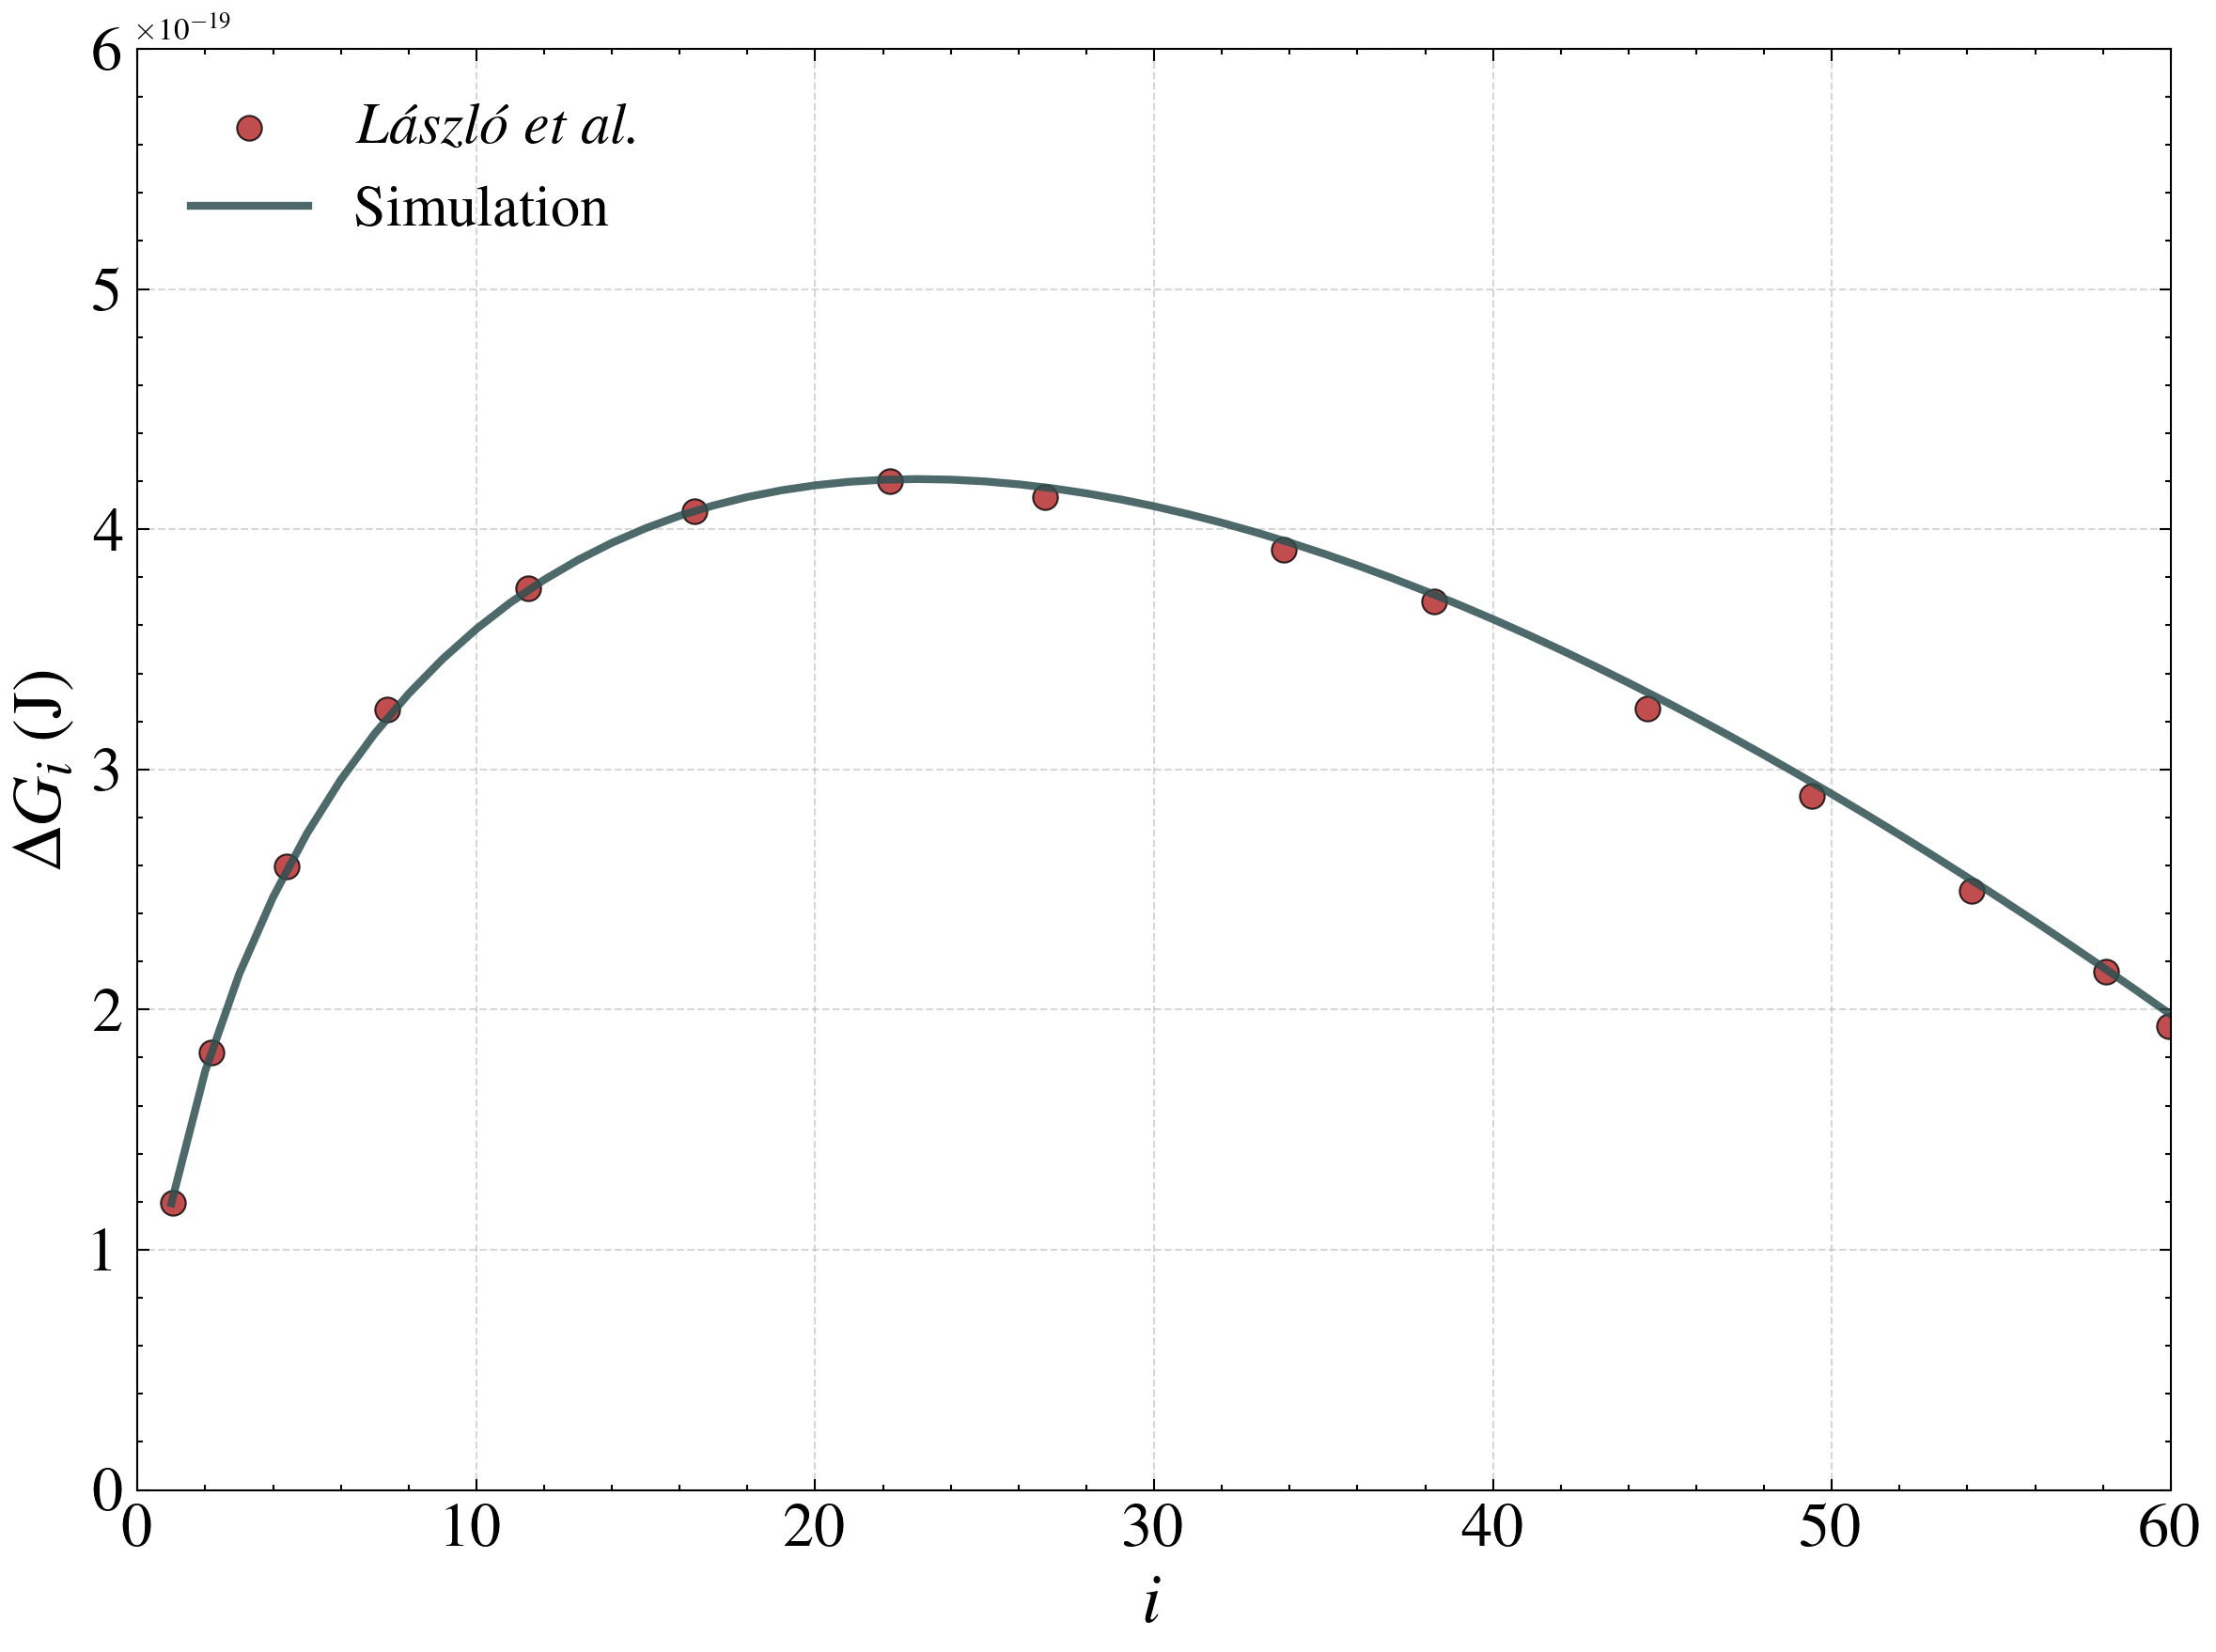
\includegraphics[width=0.9\linewidth]{laszlo_results/free_energy_comparison.png}
    \caption{Simulation and reference size dependent free energy of clusters for the uncorrected classical droplet model, CNT.}
    \label{fig:free_energy_comparison}
\end{figure}

In the case of the population distribution, the results obtained from the simulation are in perfect agreement with the reference results. 
We note the difference in the results depending on the upper boundary condition used. With the closed boundary condition the distribution is very close to the 
equilibrium distribution, for $i_{\text{max}} = 40$, since for high imax the equilibrium distribution is not fulfilled for postcritical sizes, 
as can be seen for the case of $i_{\text{max}} = 100$. 
\begin{figure}[H]
    \centering
    \hspace*{-2cm} % Adjust the -1cm to your needs
    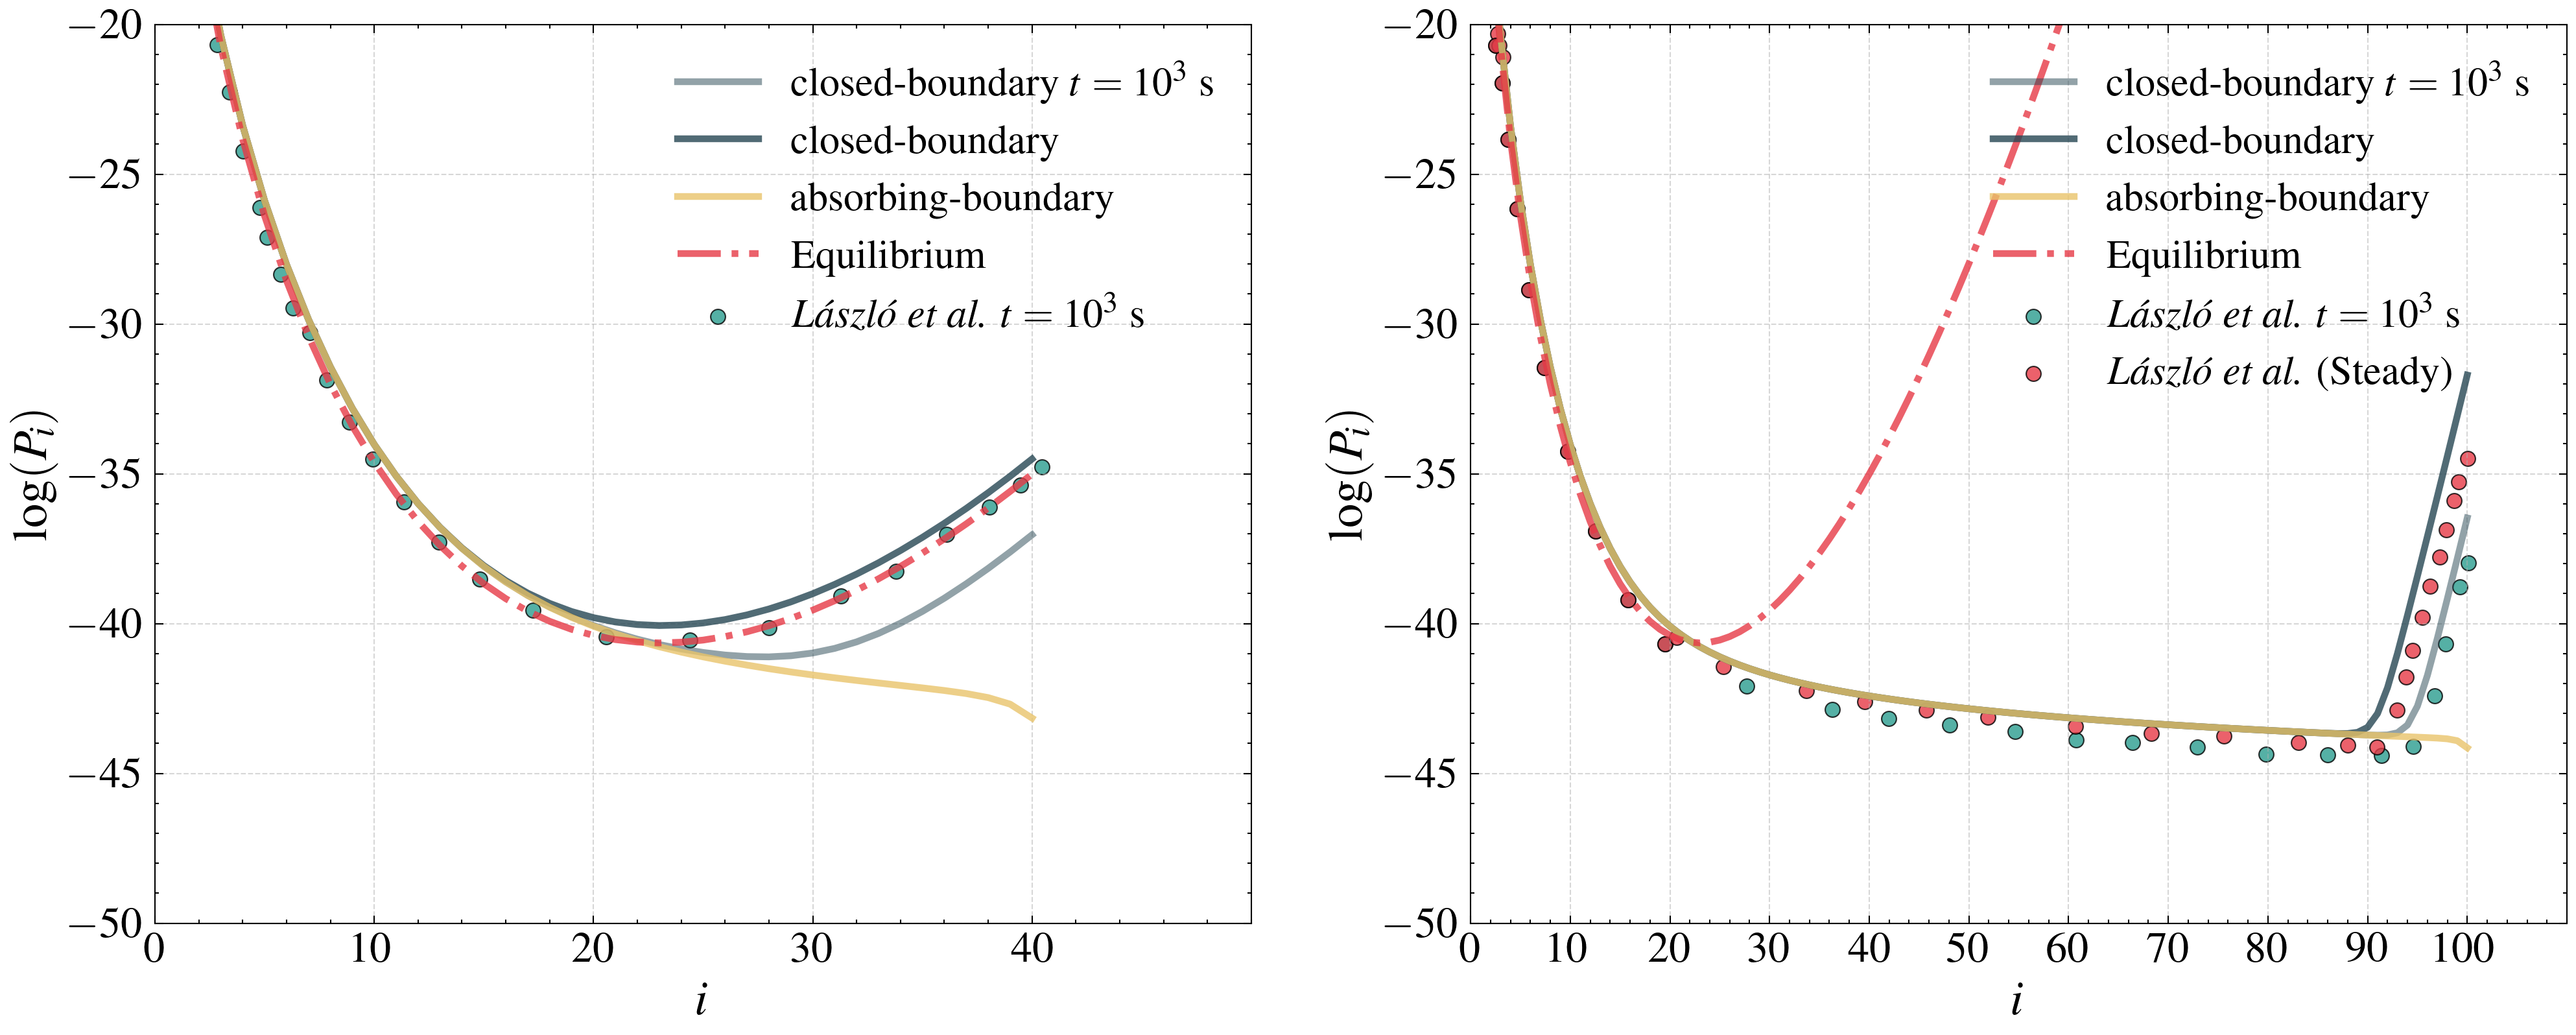
\includegraphics[width=1.2\linewidth]{laszlo_results/number_distribution.png}
    \caption{Effect of upper boundary condition comparison between simulation and reference cluster number density distribution for different sizes $i_{\text{max}} = 40$ and $100$.}
    \label{fig:number_distribution}
\end{figure}

This analysis indicates that for extended times, the number densities of supercritical clusters, obtained by summing $N_i$ and integrating the nucleation rate, match. 
In contrast, closing conditions lead to a peak in the nucleation rate before a steady state is reached, which is reflected in a drop to zero in later stages and a 
stabilization of the supercritical number densities.
Similar qualitative results were achieved for $i_{\max} = 100$ as shown in Fig. \ref{fig:number_comparison}, the steady state is reached under both boundary conditions. 
The variations emerge at larger cluster sizes and over extended durations. The accumulation at significant cluster dimensions affects the cluster population primarily 
near $i_{\max}$, marked by the exponential rise of $N_i$, requiring extensive computational efforts to achieve equilibrium for such nominal maximum sizes.

Due to the limitations of this study, where calculations are confined to $t = 10^5$ s required for reaching 
equilibrium at $i_{\max}=40$, the outcomes using the 
closing boundary condition mirror those from the absorbing-state condition, aside from a trivial area near $i_{\max}$. Nonetheless, the equivalence 
of $ N_{i > i_0} = \int_{0}^{\infty} J_{i_0} \, dt$ remains intact.

\begin{figure}[H]
    \centering
    \hspace*{-2cm} % Adjust the -1cm to your needs
    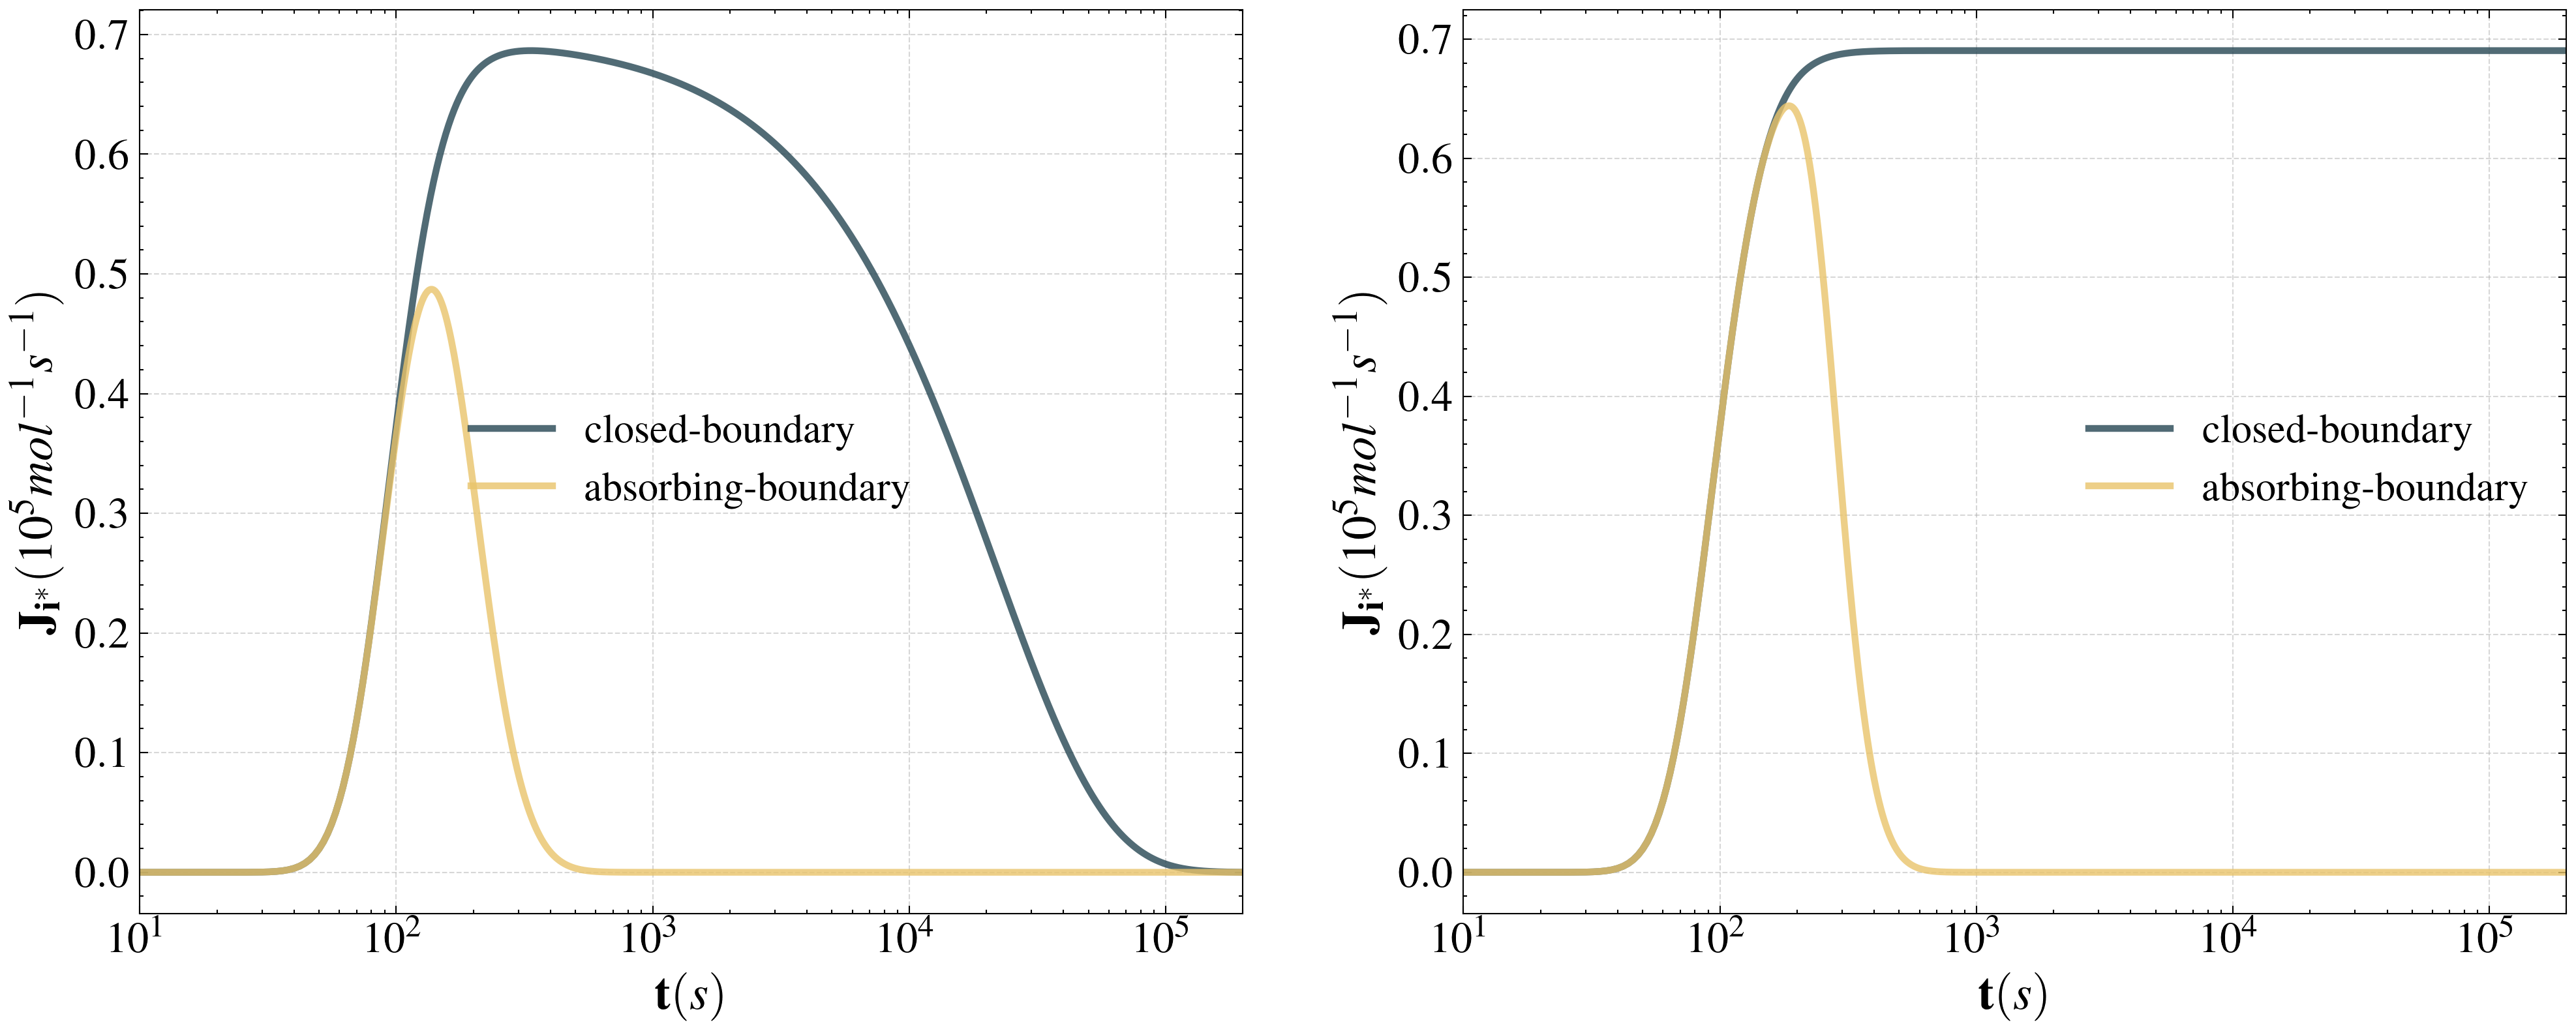
\includegraphics[width=1.2\linewidth]{laszlo_results/nucleation_rates.png}
    \caption{Effect of upper boundary condition comparison between simulation and reference postcritical nucleation rates for different sizes $i_{\text{max}} = 40$ and $100$.}
    \label{fig:nucleation_rates}
\end{figure}

\begin{figure}[H]
    \centering
    \hspace*{-2cm} % Adjust the -1cm to your needs
    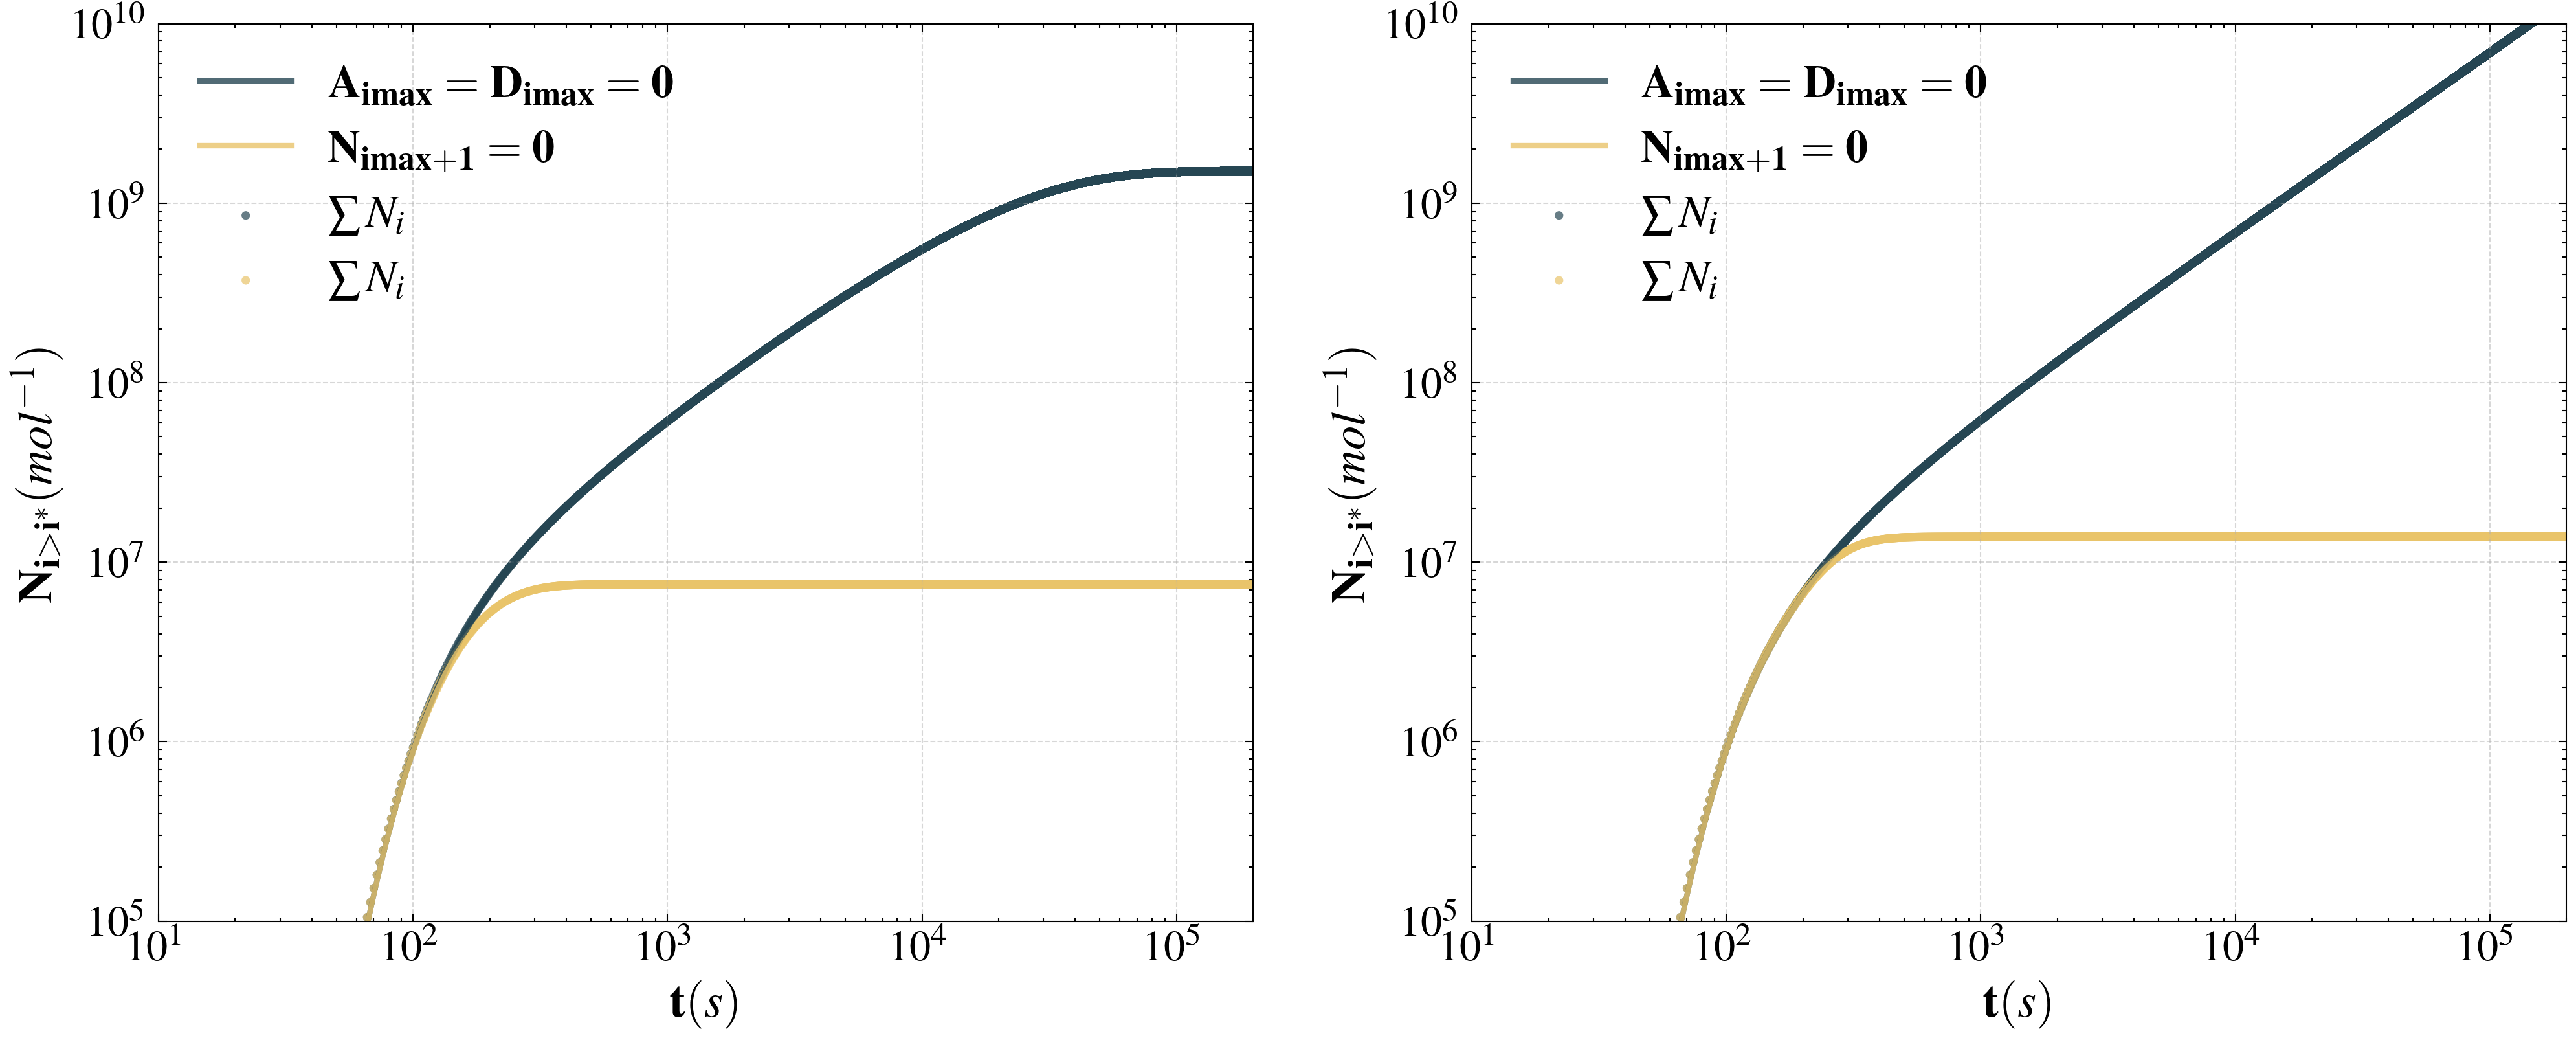
\includegraphics[width=1.2\linewidth]{laszlo_results/number_comparison.png}
    \caption{Effect of upper boundary condition comparison between simulation and reference postcritical total cluster number density for different sizes $i_{\text{max}} = 40$ and $100$.}
    \label{fig:number_comparison}
\end{figure}

To see the difference in nucleation rates for $i_{\text{max}} = 40$ and $100$ using different boundary conditions, 
the total nucleation rate for different molecule sizes is plotted.
The figures are divided as follows, on the left are the results for $i_{\text{max}} = 40$ using different upper boundary conditions, and on the right for $i_{\text{max}} = 100$.
\begin{figure}[H]
    \centering
    \hspace*{-2cm} % Adjust the -1cm to your needs
    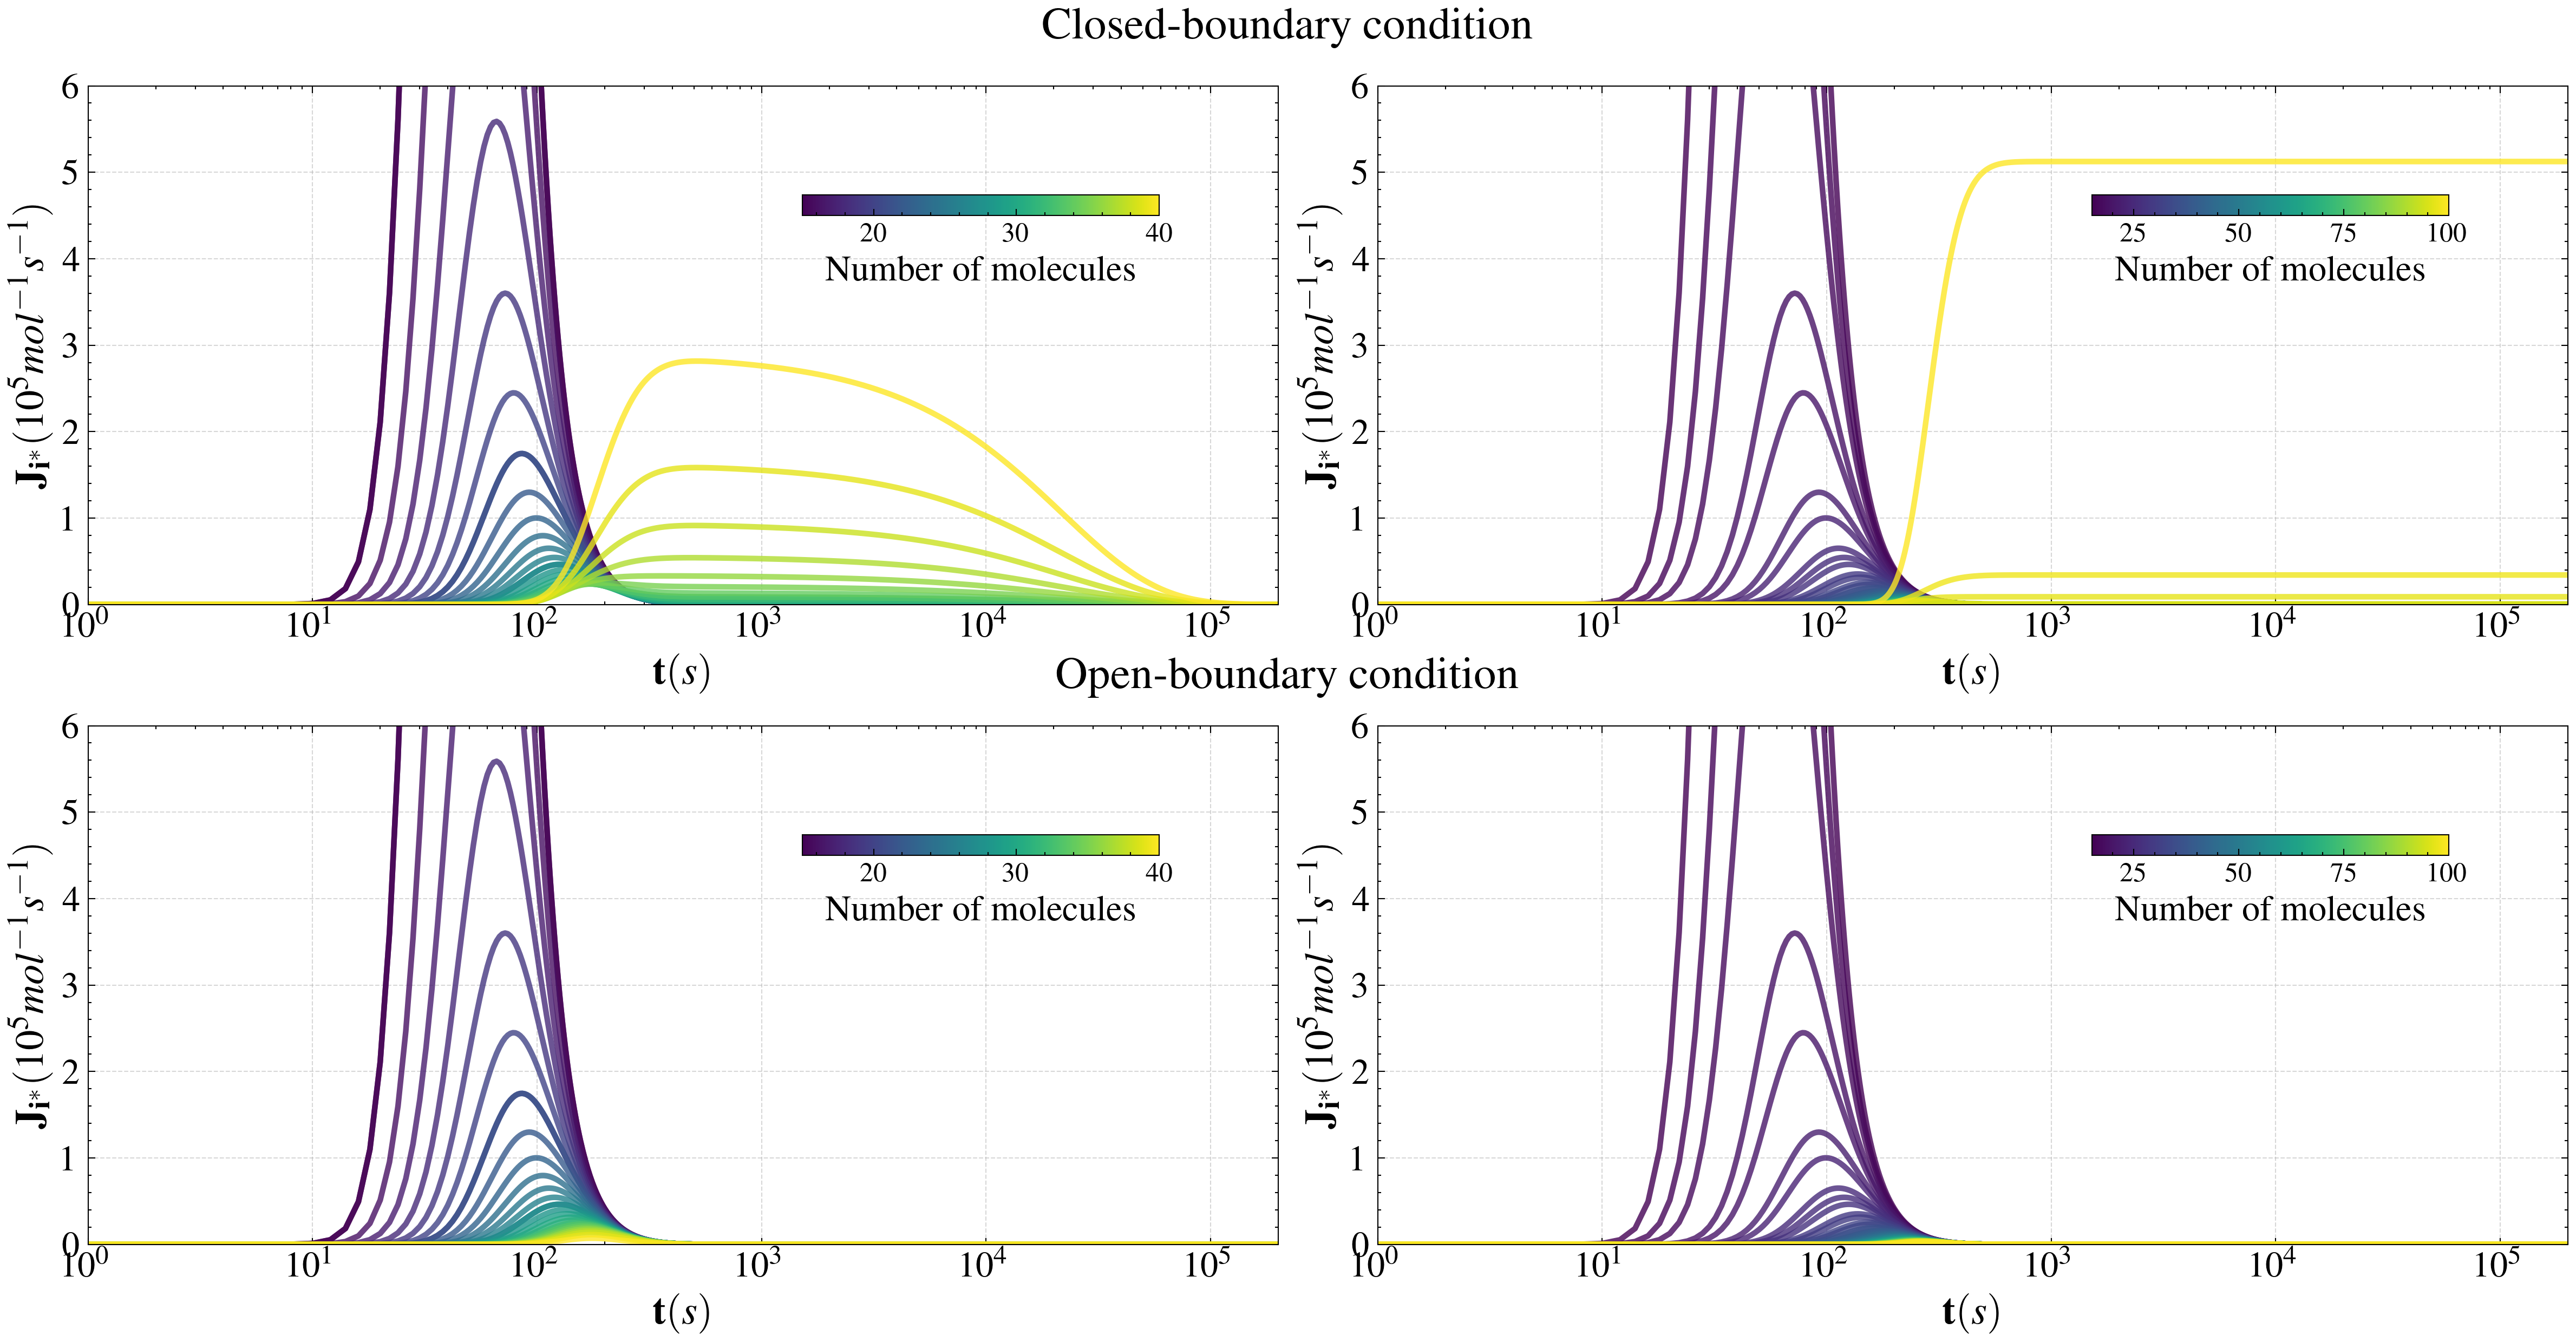
\includegraphics[width=1.2\linewidth]{laszlo_results/rate_evolution_comparison.png}
    \caption{Nucleation rates for different observable sizes for closed- boundary (top) and open-boundary(bottom) for $i_{\text{max}} = 40$ (left) and $100$ (right).}
    \label{fig:rate_evolution_comparison}
\end{figure}

The differences observed are primarily due to the boundary conditions, as previously mentioned. In scenarios with closed boundary conditions, there 
is an accumulation of large clusters, resulting in a higher nucleation rate compared to clusters of intermediate sizes.

Additionally, it has been noted that when the maximum cluster size $i_{\text{max}}$ increases, the behavior of the curve changes to an exponential form, maintaining a 
constant value at the steady state. This is in contrast to a maximum size of $i_{\text{max}} = 40$, where the rate tends to zero, thereby mirroring the equilibrium distribution more closely.

From these observations, we can deduce that for smaller maximum sizes, the stationary population distribution aligns more closely with the equilibrium distribution. 
However, as the maximum size expands, the stationary distribution begins to diverge from the equilibrium state.

\begin{figure}[H]
    \centering
    \hspace*{-2cm} % Adjust the -1cm to your needs
    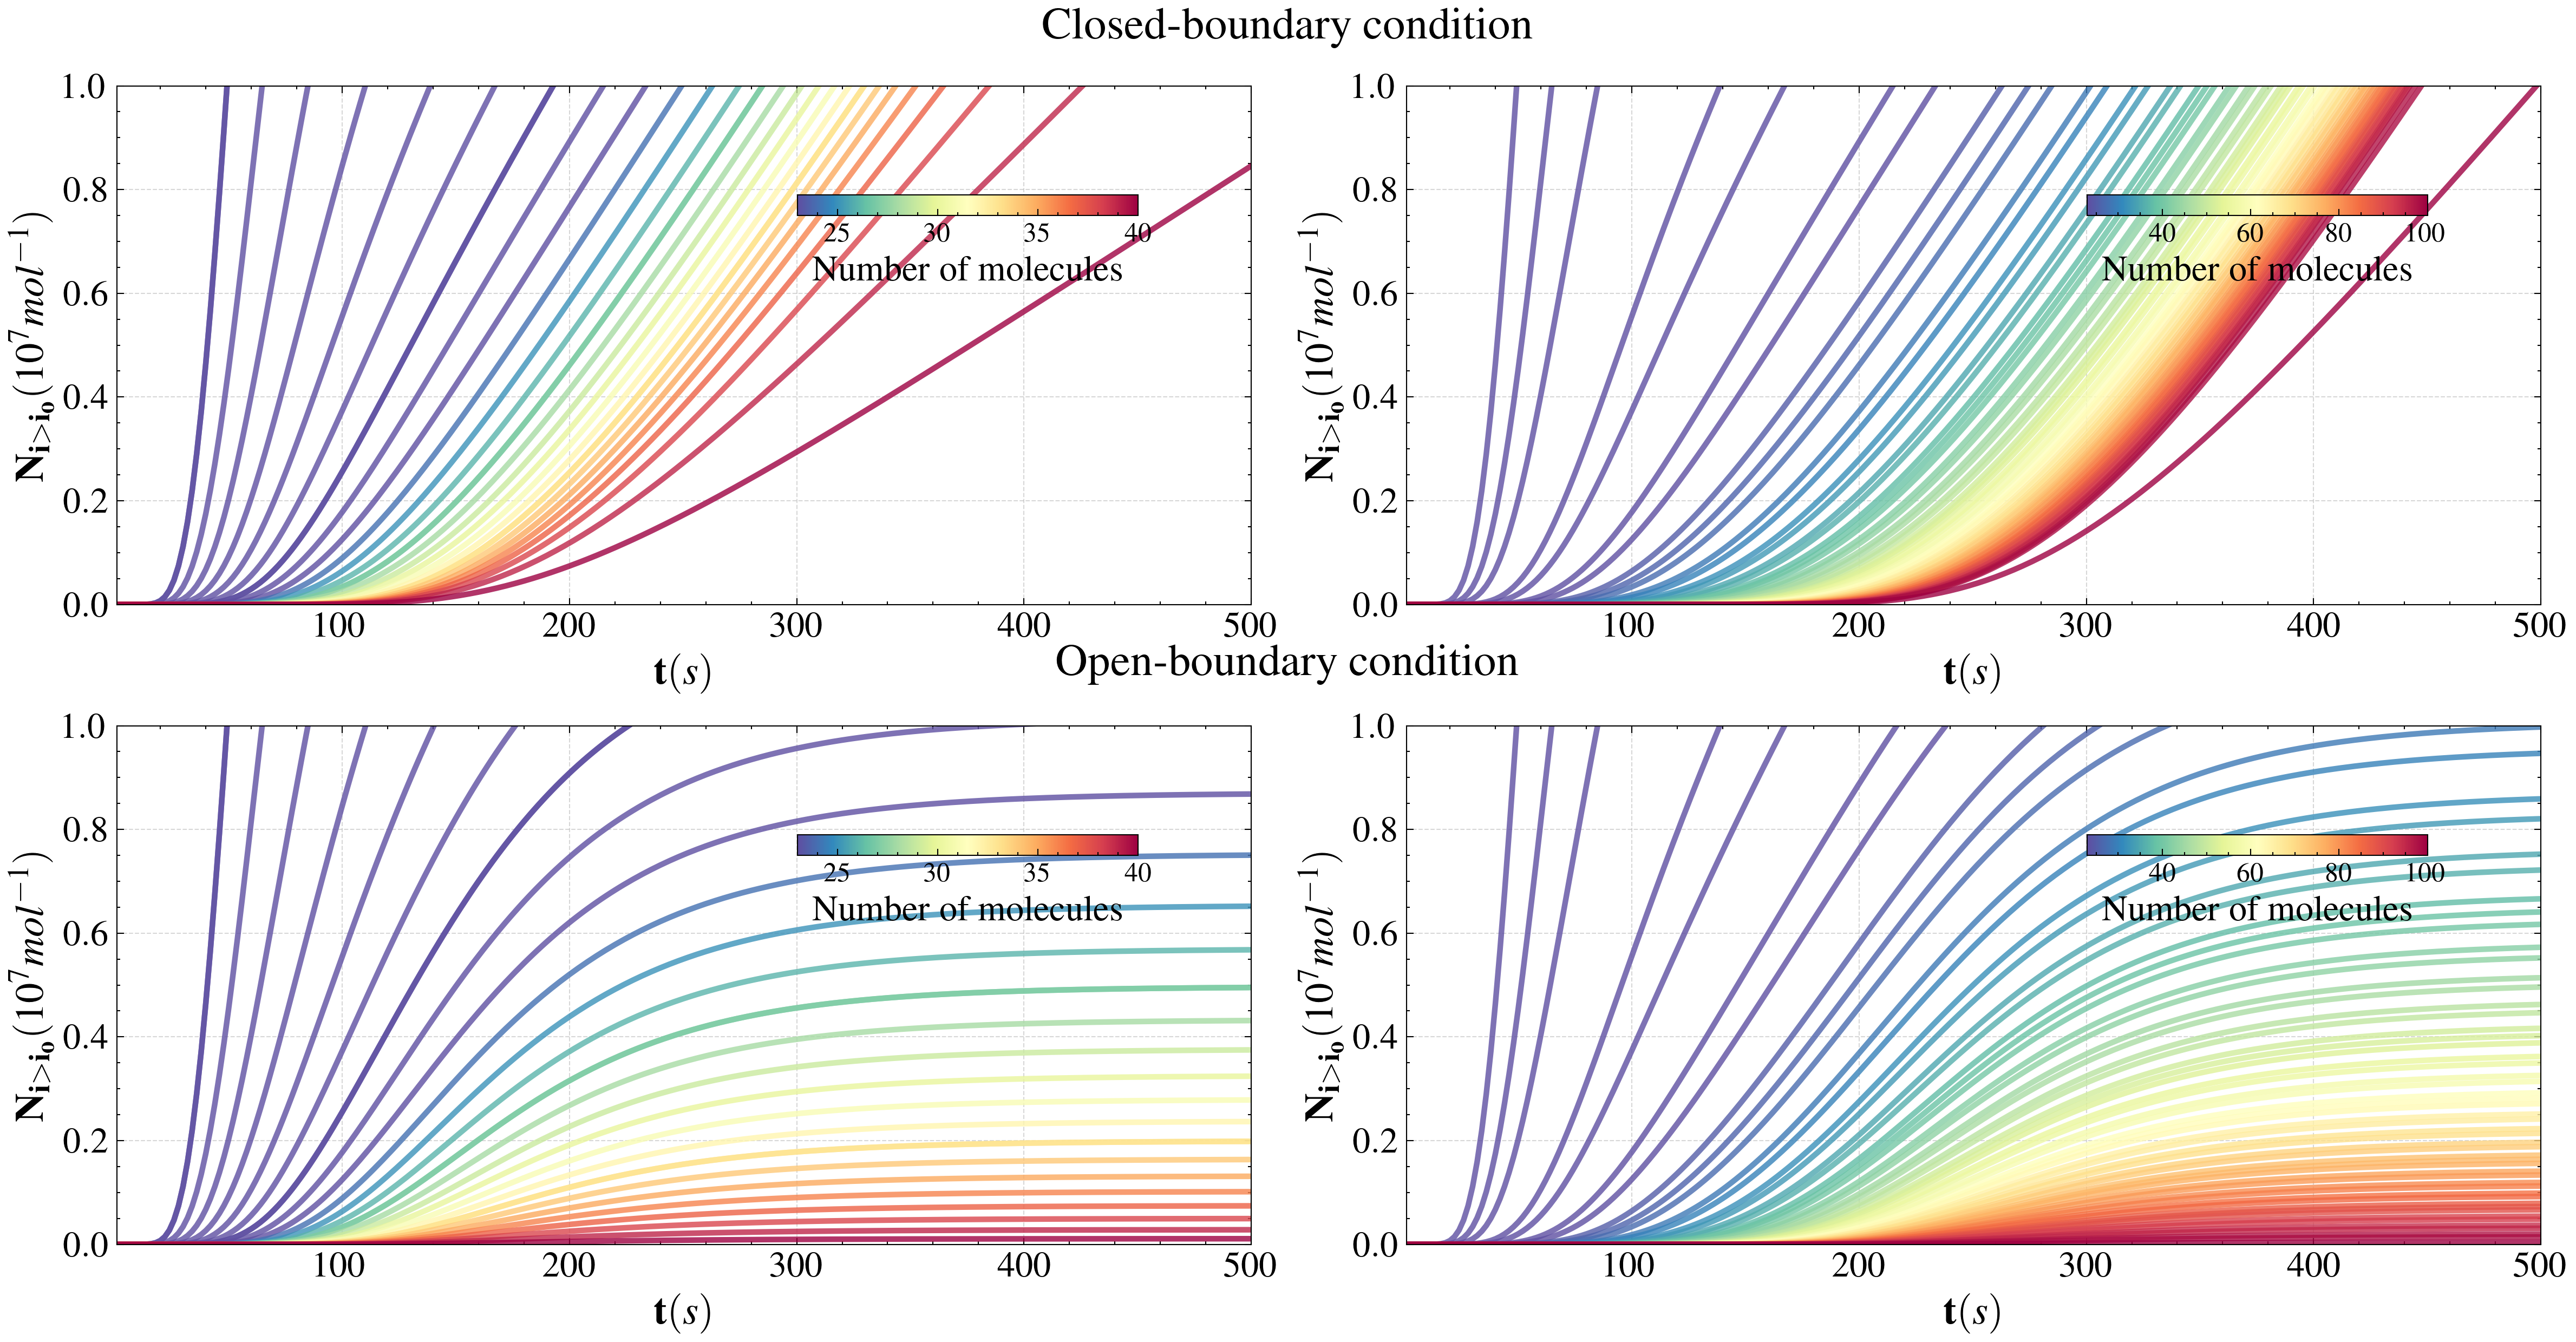
\includegraphics[width=1.2\linewidth]{laszlo_results/number_evolution_comparison.png}
    \caption{Total number density for different observable sizes for closed- boundary (top) and open-boundary(bottom) for $i_{\text{max}} = 40$ (left) and $100$ (right).}
    \label{fig:number_evolution_comparison}
\end{figure}

In the case of number density, for open boundary conditions, a steady state is reached more quickly than for closed conditions.

\subsection{Impurities results}
In this section we will summarise the thermodynamic parameters found for each impurity and the results obtained from simulation.
The section is then divided into metallic and non-metallic impurities. 
\subsubsection{Metallic impurities}
In this section the data and results for metallic impurities (Fe, Cr, AlN) are presented.
\paragraph{Fe}~\\
\vspace{1mm} % Adjust the space as needed
First of all, the most important thing to consider is which phases are present in the Li-Fe system at the temperature at 
which this fluid will be found.The phase diagram of the Fe-Li system is obtained from FactSage database \cite{Bale2016}, where also allows 
equilibrium calculations for some systems.
\begin{figure}[H]
    \centering
    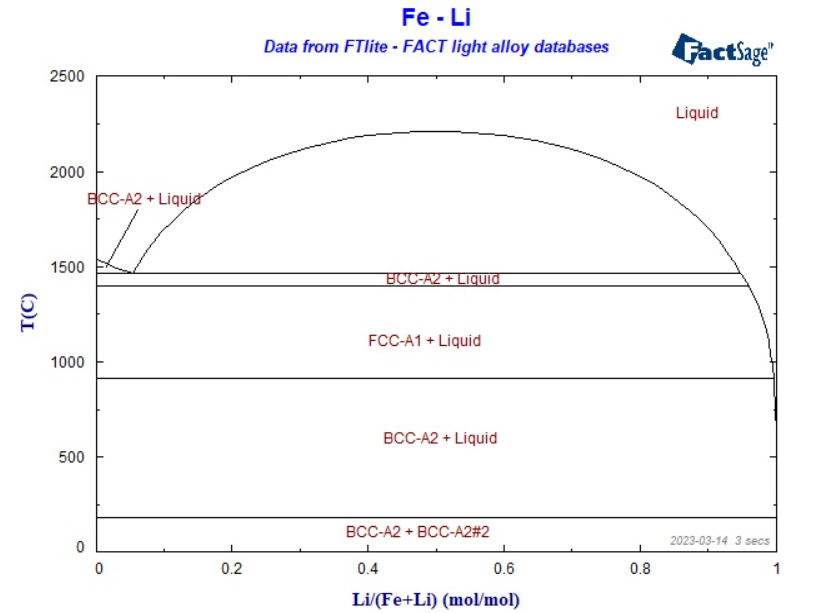
\includegraphics[width=0.9\linewidth]{Fe-Li_phase_diagram.png}
    \caption{Phase diagram of Li-Fe mixture from FactSage database \cite{Bale2016}.}
    \label{fig:fe_li_diagram}
\end{figure}

From \cite{Leavenworth1961TheSO} the solubility of Fe in Li is extracted ad different temperatures and then fitting the data. In the Fig. \ref{fig:Fe_solubility} the solubility of Fe in Li is shown.
\begin{figure}[H]
    \centering
    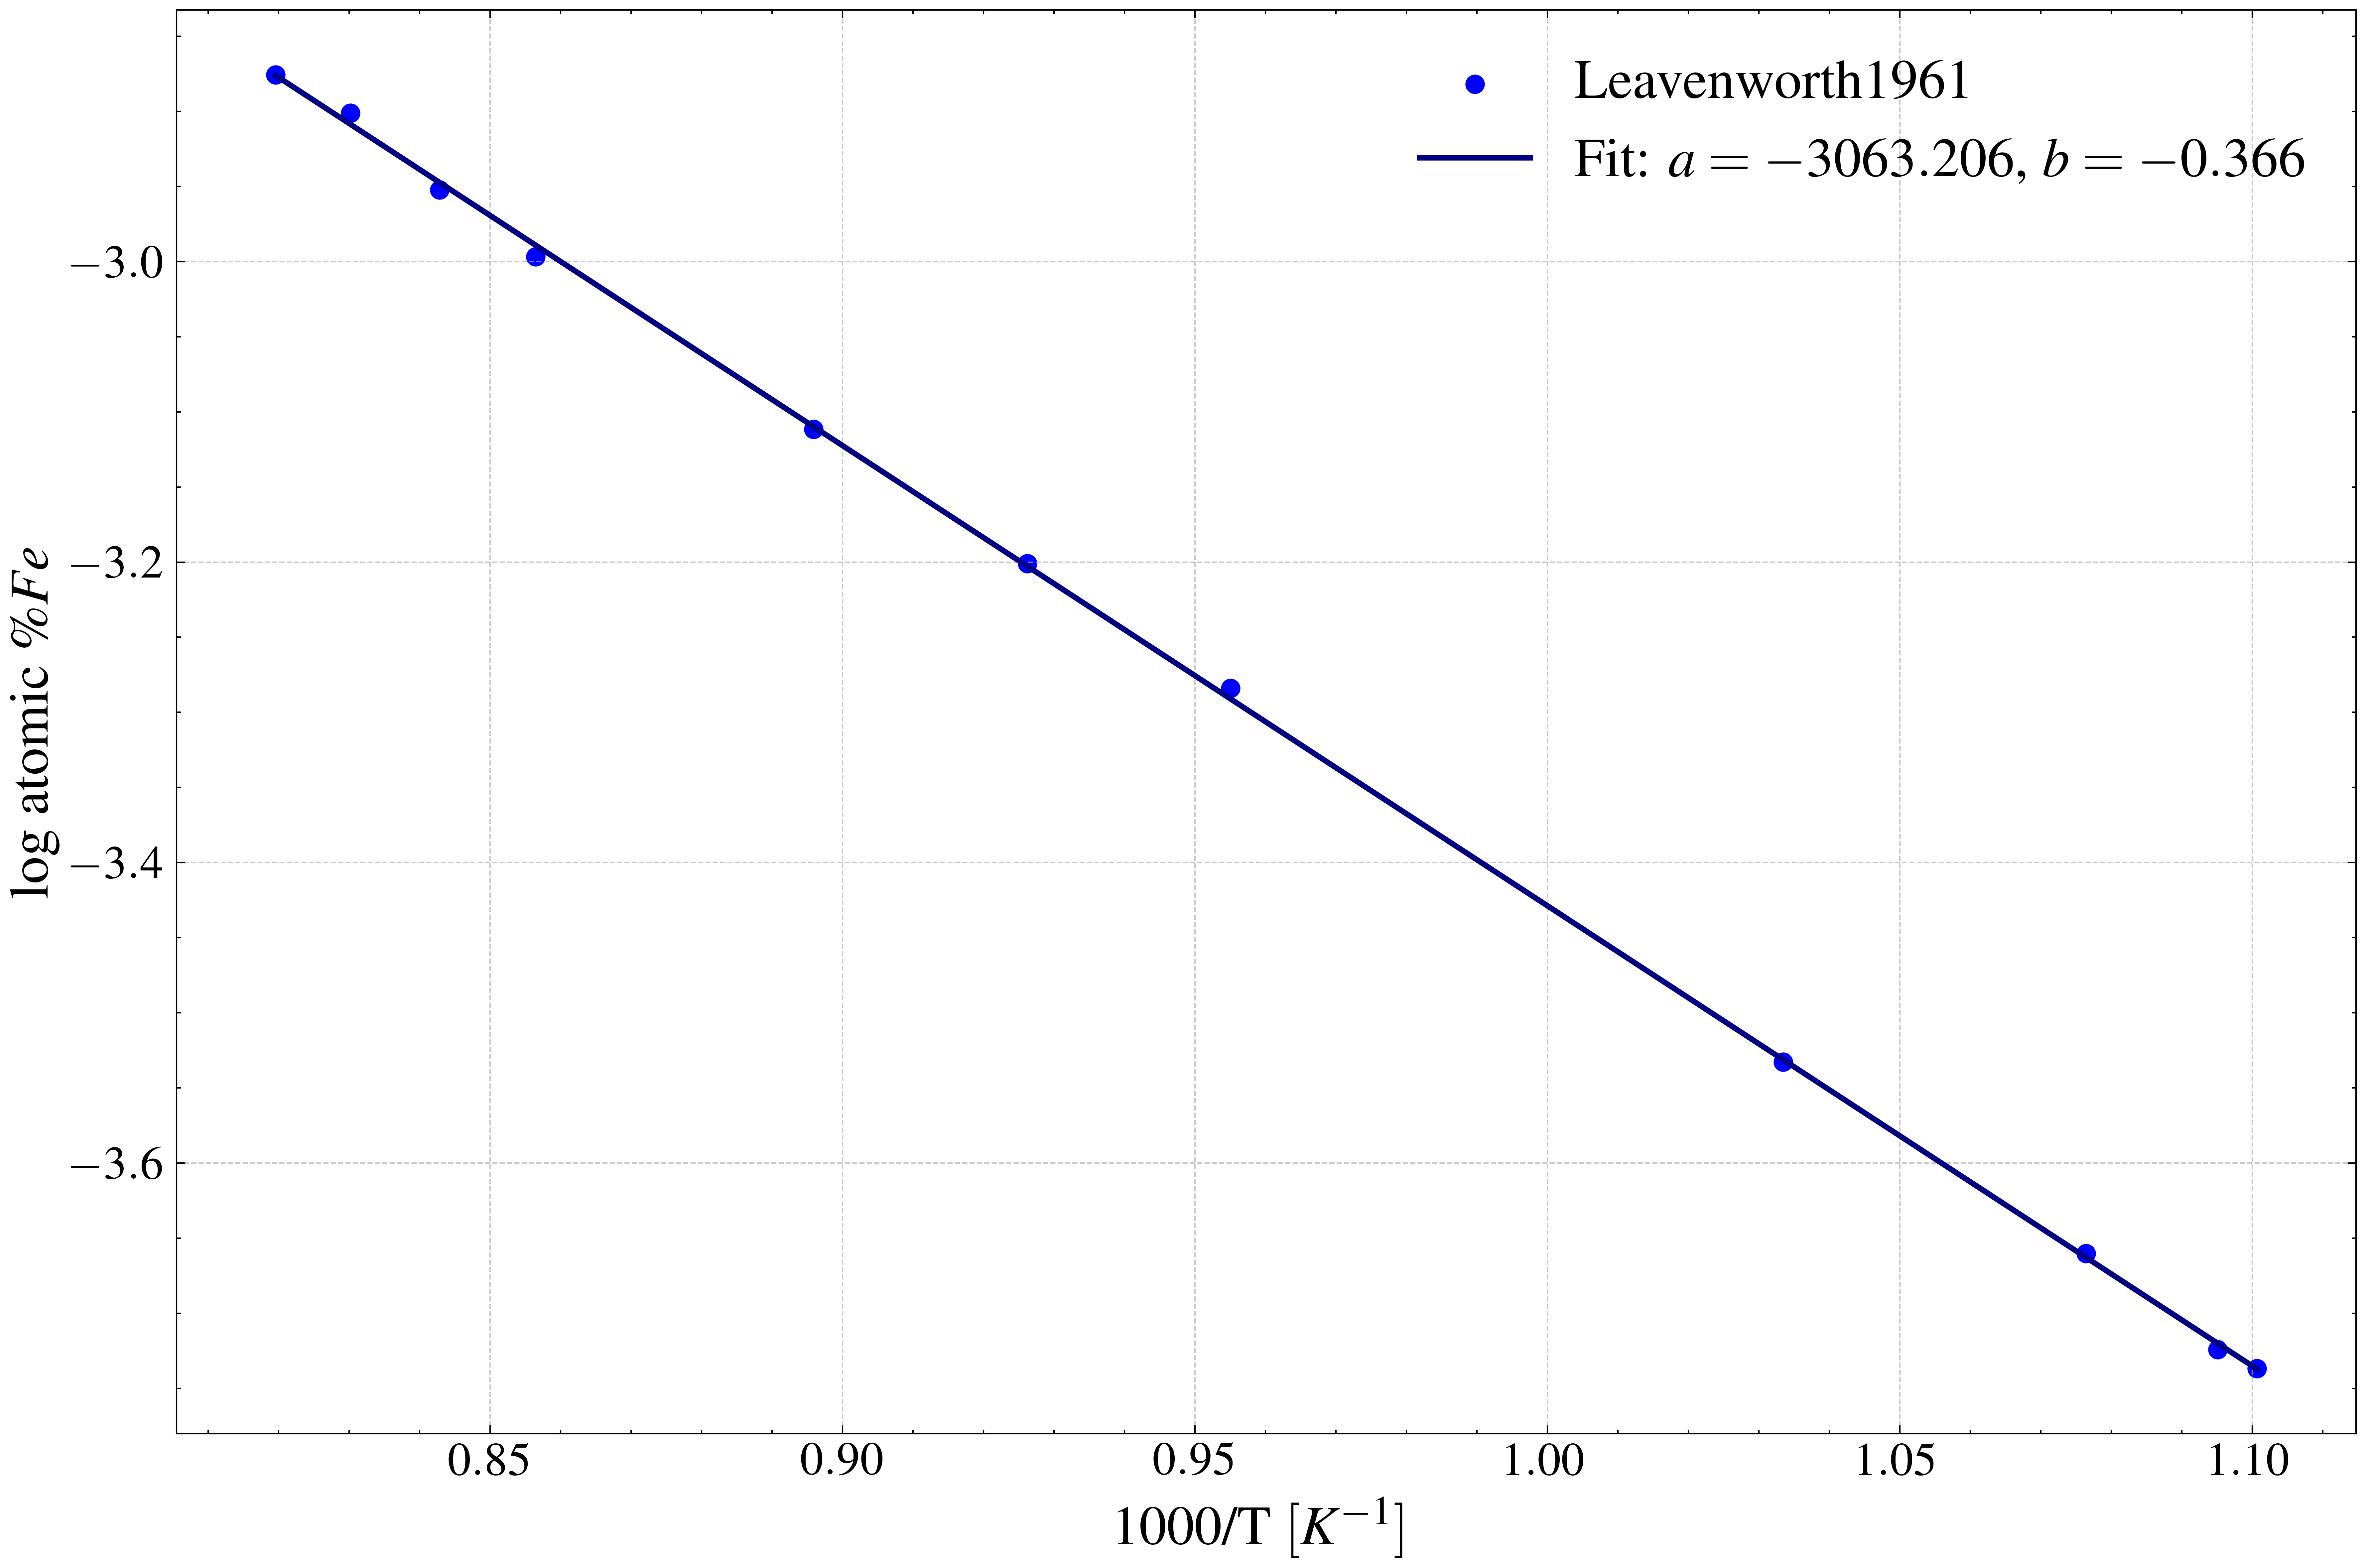
\includegraphics[width=0.9\linewidth]{Fe_solubility.png}
    \caption{Fe solubility in liquid lithium dependence on temperature \ref{Leavenworth1961TheSO}. }
    \label{fig:Fe_solubility}
\end{figure}

As previously mentioned, FactSage allows equilibrium calculations to be made for certain systems, in this case, for the Fe-Li system, it has been 
possible to calculate equilibrium compositions for the operating temperature and subsequently 
comparing the solubility of the reference with the calculated parameters.

\begin{table}[ht]
	\centering
	\label{tab:your_label_here}
	\begin{tabular}{ccc}
	\hline
	$Reference$ & $x^{\text{A}}_{l,eq}$ & $x^{\text{A}}_{s,eq}$ \\ \hline
	FactSage \cite{Bale2016} & $1.76 \times 10^{-5} $        & $1.00$         \\
	Ref. \cite{Leavenworth1961TheSO}       & $1.12 \times 10^{-5}$         & -         \\
	\end{tabular}
	\caption{Equilibrium compositions of iron using FactSage and reference data.}
\end{table}

The findings closely match and share the same order of magnitude, indicating consistency in the values. In the table below, we 
display the balanced compositions calculated with FactSage for specific values: first, the initial values used, and then, those slightly increased.

\begin{table}[ht]
	\centering
	\label{tab:updated_stream_phases}
	\begin{tabular}{lccc}
	\hline
	\multicolumn{4}{c}{Molar fractions (T = 668 K)} \\
	\hline
	Species & Amount/mol & & \\
	\hline
	Fe & $1.6000 \times 10^{-7}$ & & \\
	Li & $1.0000 \times 10^{0}$ & & \\
	\hline
	\multicolumn{4}{c}{PHASE: Liquid\#1(\#2)} \\
	\hline
	Species & Amount/mol & Mole Fraction & Activity \\
	\hline
	Fe & $1.6000 \times 10^{-7}$ & $1.6000 \times 10^{-7}$ & $1.3491 \times 10^{-3}$ \\
	Li & $1.0000 \times 10^{0}$ & $1.0000 \times 10^{0}$ & $1.0000 \times 10^{0}$ \\
	Total & $1.0000 \times 10^{0}$ & $1.0000$ & $1.0000$ \\
	\hline
	\multicolumn{4}{c}{PHASE: BCC-A2\#1} \\
	\hline
	Species & Amount/mol & Mole Fraction & Activity \\
	\hline
	Fe-alpha & $0.0000 \times 10^{0}$ & $5.6693 \times 10^{-16}$ & $9.1079 \times 10^{-3}$ \\
	Li & $0.0000 \times 10^{0}$ & $1.0000$ & $7.7433 \times 10^{-1}$ \\
	Total & $0.0000 \times 10^{0}$ & $1.0000$ & $7.7433 \times 10^{-1}$ \\
	\hline
	\end{tabular}
	\caption{Equilibrium compositions of iron using FactSage with an iron molar fraction used as input.}

\end{table}
	
\begin{table}[ht]
	\centering
	\label{tab:stream_phases}
	\begin{tabular}{lccc}
	\hline
	\multicolumn{2}{c}{Molar fractions (T = 668 K)} \\
	\hline
	Species & Amount/mol  \\
	\hline
	Fe & $9.2880 \times 10^{-5}$  \\
	Li & $9.9991 \times 10^{-1}$  \\
	\hline
	\multicolumn{4}{c}{PHASE: Liquid\#1} \\
	\hline
	Species & Amount/mol & Mole Fraction & Activity \\
	\hline
	Fe & $1.7601 \times 10^{-5}$ & $1.7603 \times 10^{-5}$ & $1.4813 \times 10^{-1}$ \\
	Li & $9.9991 \times 10^{-1}$ & $9.9998 \times 10^{-1}$ & $9.9998 \times 10^{-1}$ \\
	Total & $9.9992 \times 10^{-1}$ & $1.0000$ & $1.0000$ \\
	\hline
	\multicolumn{4}{c}{PHASE: BCC-A2\#1} \\
	\hline
	Species & Amount/mol & Mole Fraction & Activity \\
	\hline
	Fe-alpha & $7.5279 \times 10^{-5}$ & $1.0000$ & $1.0000$ \\
	Li & $1.3112 \times 10^{-18}$ & $1.7418 \times 10^{-14}$ & $7.7432 \times 10^{-1}$ \\
	Total & $7.5279 \times 10^{-5}$ & $1.0000$ & $1.0000$ \\
	\hline
	\end{tabular}
	\caption{Equilibrium compositions of iron using FactSage with an iron molar fraction increased to $x^{\text{A}}_{l} = 9.2880 \times 10^{-5}$.}
\end{table}
		
From these results, several conclusions can be drawn. Initially, it is evident that employing the 
assumed mole fraction as input results in the presence of only one liquid phase, thereby intersecting 
with the equilibrium state. This is a significant observation as it highlights the system's state under the given conditions.

In an enhanced analysis, as illustrated by the second table, an increase in the mole fraction leads to the liquid 
phase reaching the equilibrium fraction of iron, equivalent to its solubility limit. Conversely, in the solid phase 
that subsequently forms, it is observed to be entirely composed of iron. This finding is critical as it suggests that, 
based on the mole fraction initially used for the input, iron is insoluble in lithium at the specified operating temperature.

Consequently, to determine the driving force, the formalism from Eq. \ref{eq:simplified_free_energy_change} is used, considering that the solid fraction is 
entirely constituted by one of the mixture's elements. Similarly, for calculating the surface energy, the Eq. \ref{eq:Thompson_Spaepen_model} is employed.

The following table provides a summary of the obtained and identified values, which are essential for calculating the size distribution of the clusters. 
The diffusivity of iron in liquid lithium has not been found, and therefore, the diffusivity of chromium in Pb-Li has been used for both iron and chromium \cite{KHANCHYCH2023101527}.
\begin{table}[h]
    \centering
    \begin{tabular}{|l|l|l|}
    \hline
    \textbf{Parameter} & \textbf{Symbol} & \textbf{Value (Unit)} \\ \hline
    Temperature        & $T$             & 668 K                 \\ \hline
    Molar Mass         & $M$             & 55.85 g/mol         \\ \hline
    Mass Density       & $\rho$          & 7.87 g/cm$^3$         \\ \hline
    Melting Point      & $T_m$           & 1811 K                \\ \hline
    Heat of Fusion     & $\Delta H_f$    & 13.8 kJ/mol           \\ \hline
    Surface Tension    & $\sigma$        & 0.11 J/m$^2$          \\ \hline
	Diffusion Coefficient & $D$          & $4 \times 10^{-14}$ m$^2$/s \\ \hline
    \end{tabular}
    \caption{Parameters for Fe}
    \label{tab:params_Fe}
\end{table}

In Table. \ref{tab:critical_fe} the critical parameters are obtained.
\begin{table}[h]
	\centering
	\begin{tabular}{|l|l|l|}
	\hline
	\textbf{Parameter} & \textbf{Symbol} & \textbf{Value (Unit)} \\ \hline
	Critical radius        & $r^*$             & 0.35 nm                 \\ \hline
	Energy barrier         & $\Delta G^*$             & $4.22 \times 10^{-19}$ J         \\ \hline
	Critical number of molecules       & $n^*$          & 114         \\ \hline
	\end{tabular}
	\caption{Critical values for Fe}
	\label{tab:critical_fe}
\end{table}

To solve the system of kinetic equations and obtain the size distribution, we utilized the model described in the previous section. 
A closed boundary condition was selected for this purpose. Additionally, as a pre-exponential factor $N_0$ for the equilibrium distribution, 
the Avogadro number $N_A$ was employed, consistent with methodologies used in prior benchmarking, ensuring that the results are expressed per mole. 
Furthermore, the jump rate $\lambda$ has been defined as the cubic root of the solid's molecular volume.
In this case, we have chosen to perform simulations with molecule sizes larger than $3*n^*$, normally used in these kind of calculations. In the 
following graph we can see the size distribution for $i_{max}=400$ and $i_{max}=900$.

\begin{figure}[H]
    \centering
    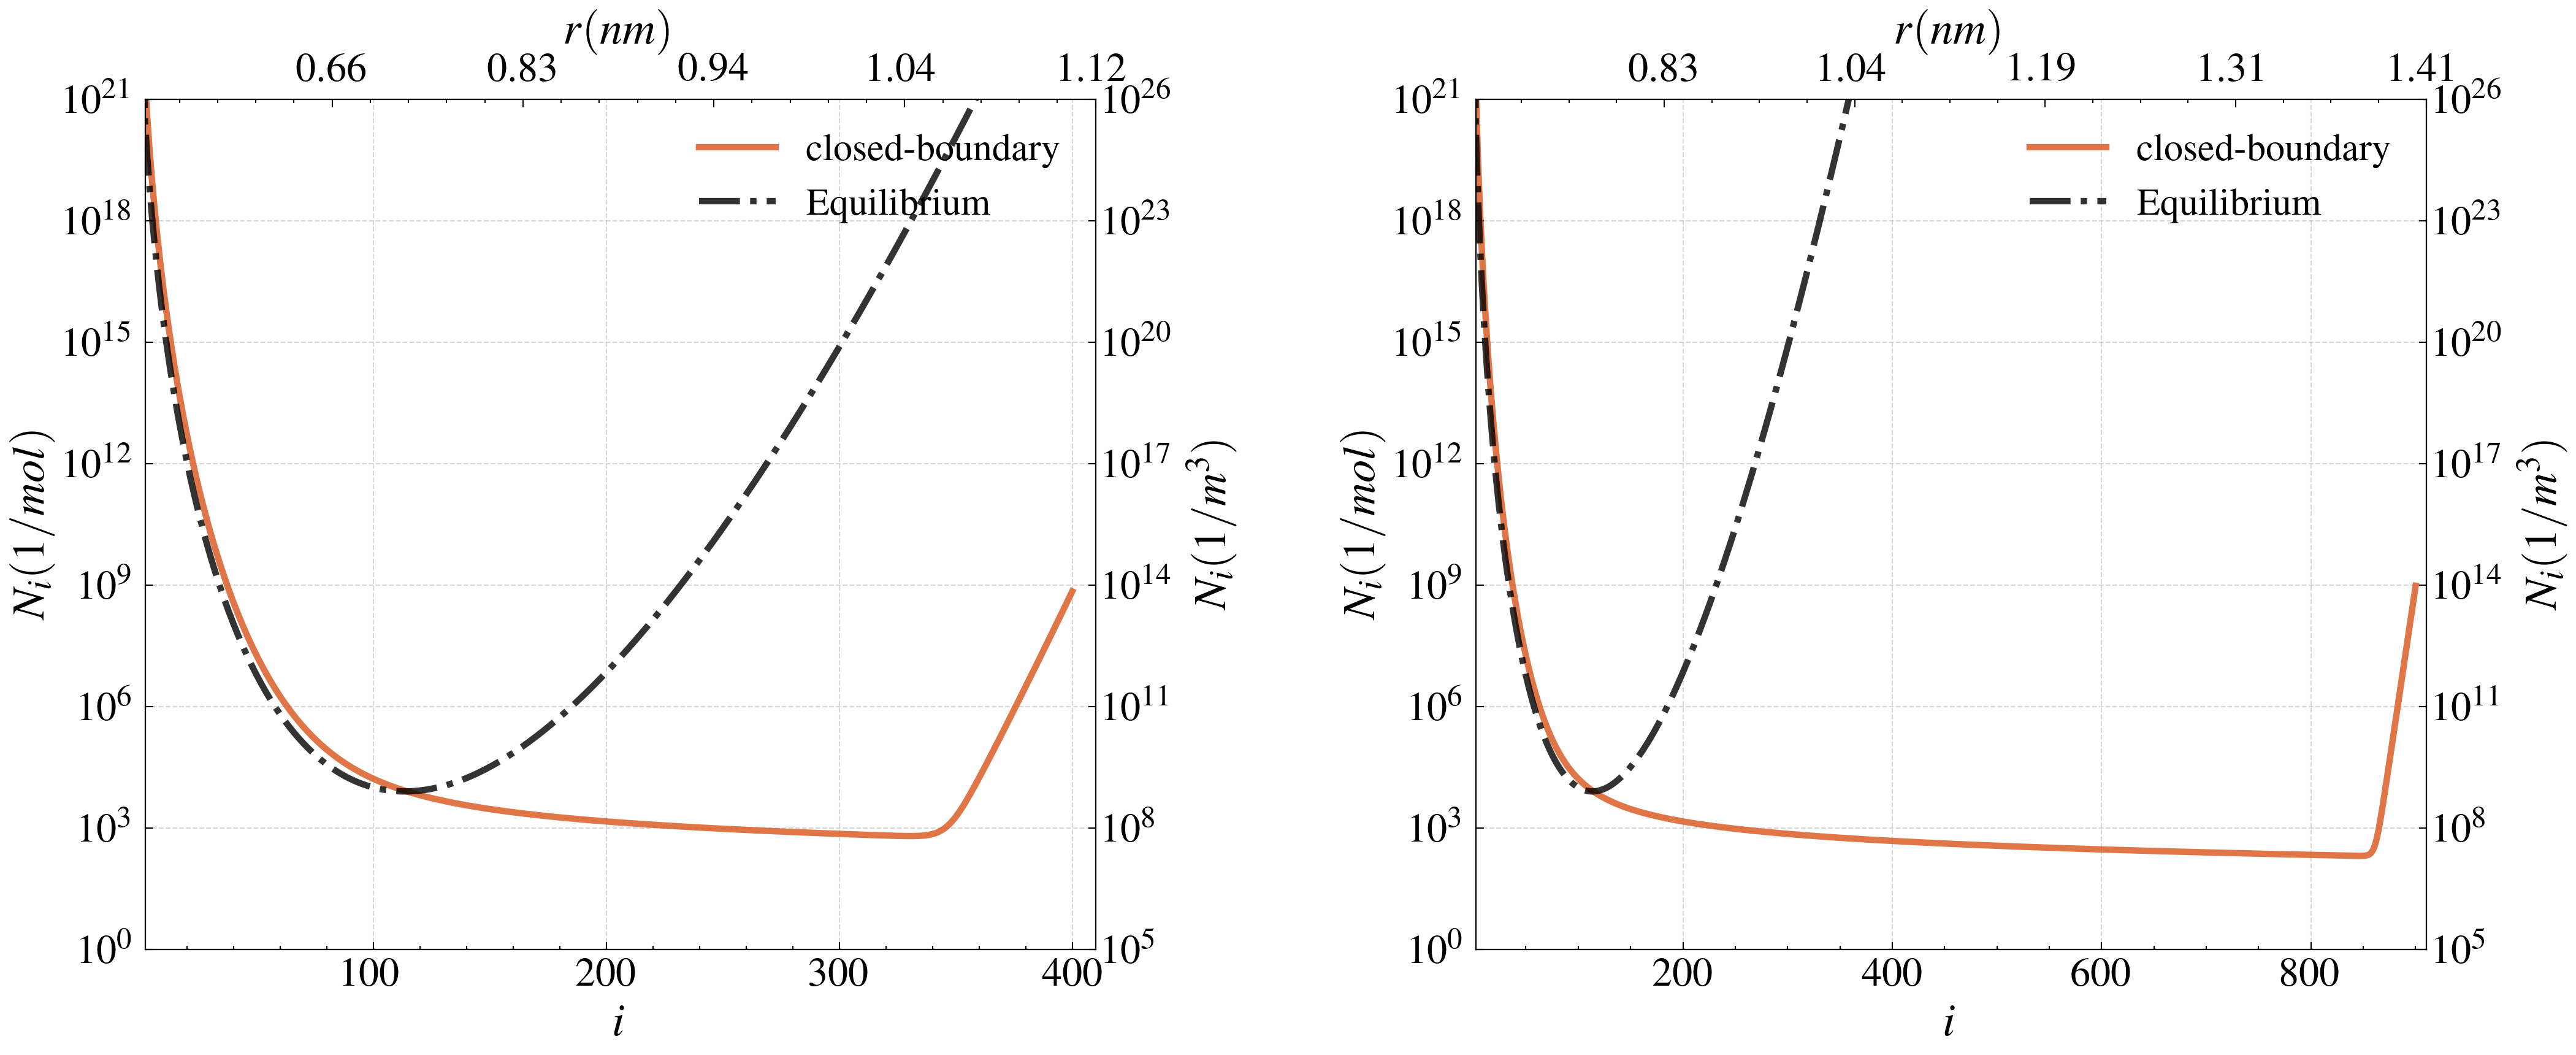
\includegraphics[width=1.1\linewidth]{psd_iron.png}
    \caption{Iron cluster number density distribution for different sizes $i_{\text{max}} = 400$ and $900$.}
    \label{fig:psd_iron}
\end{figure}

\begin{figure}[H]
    \centering
    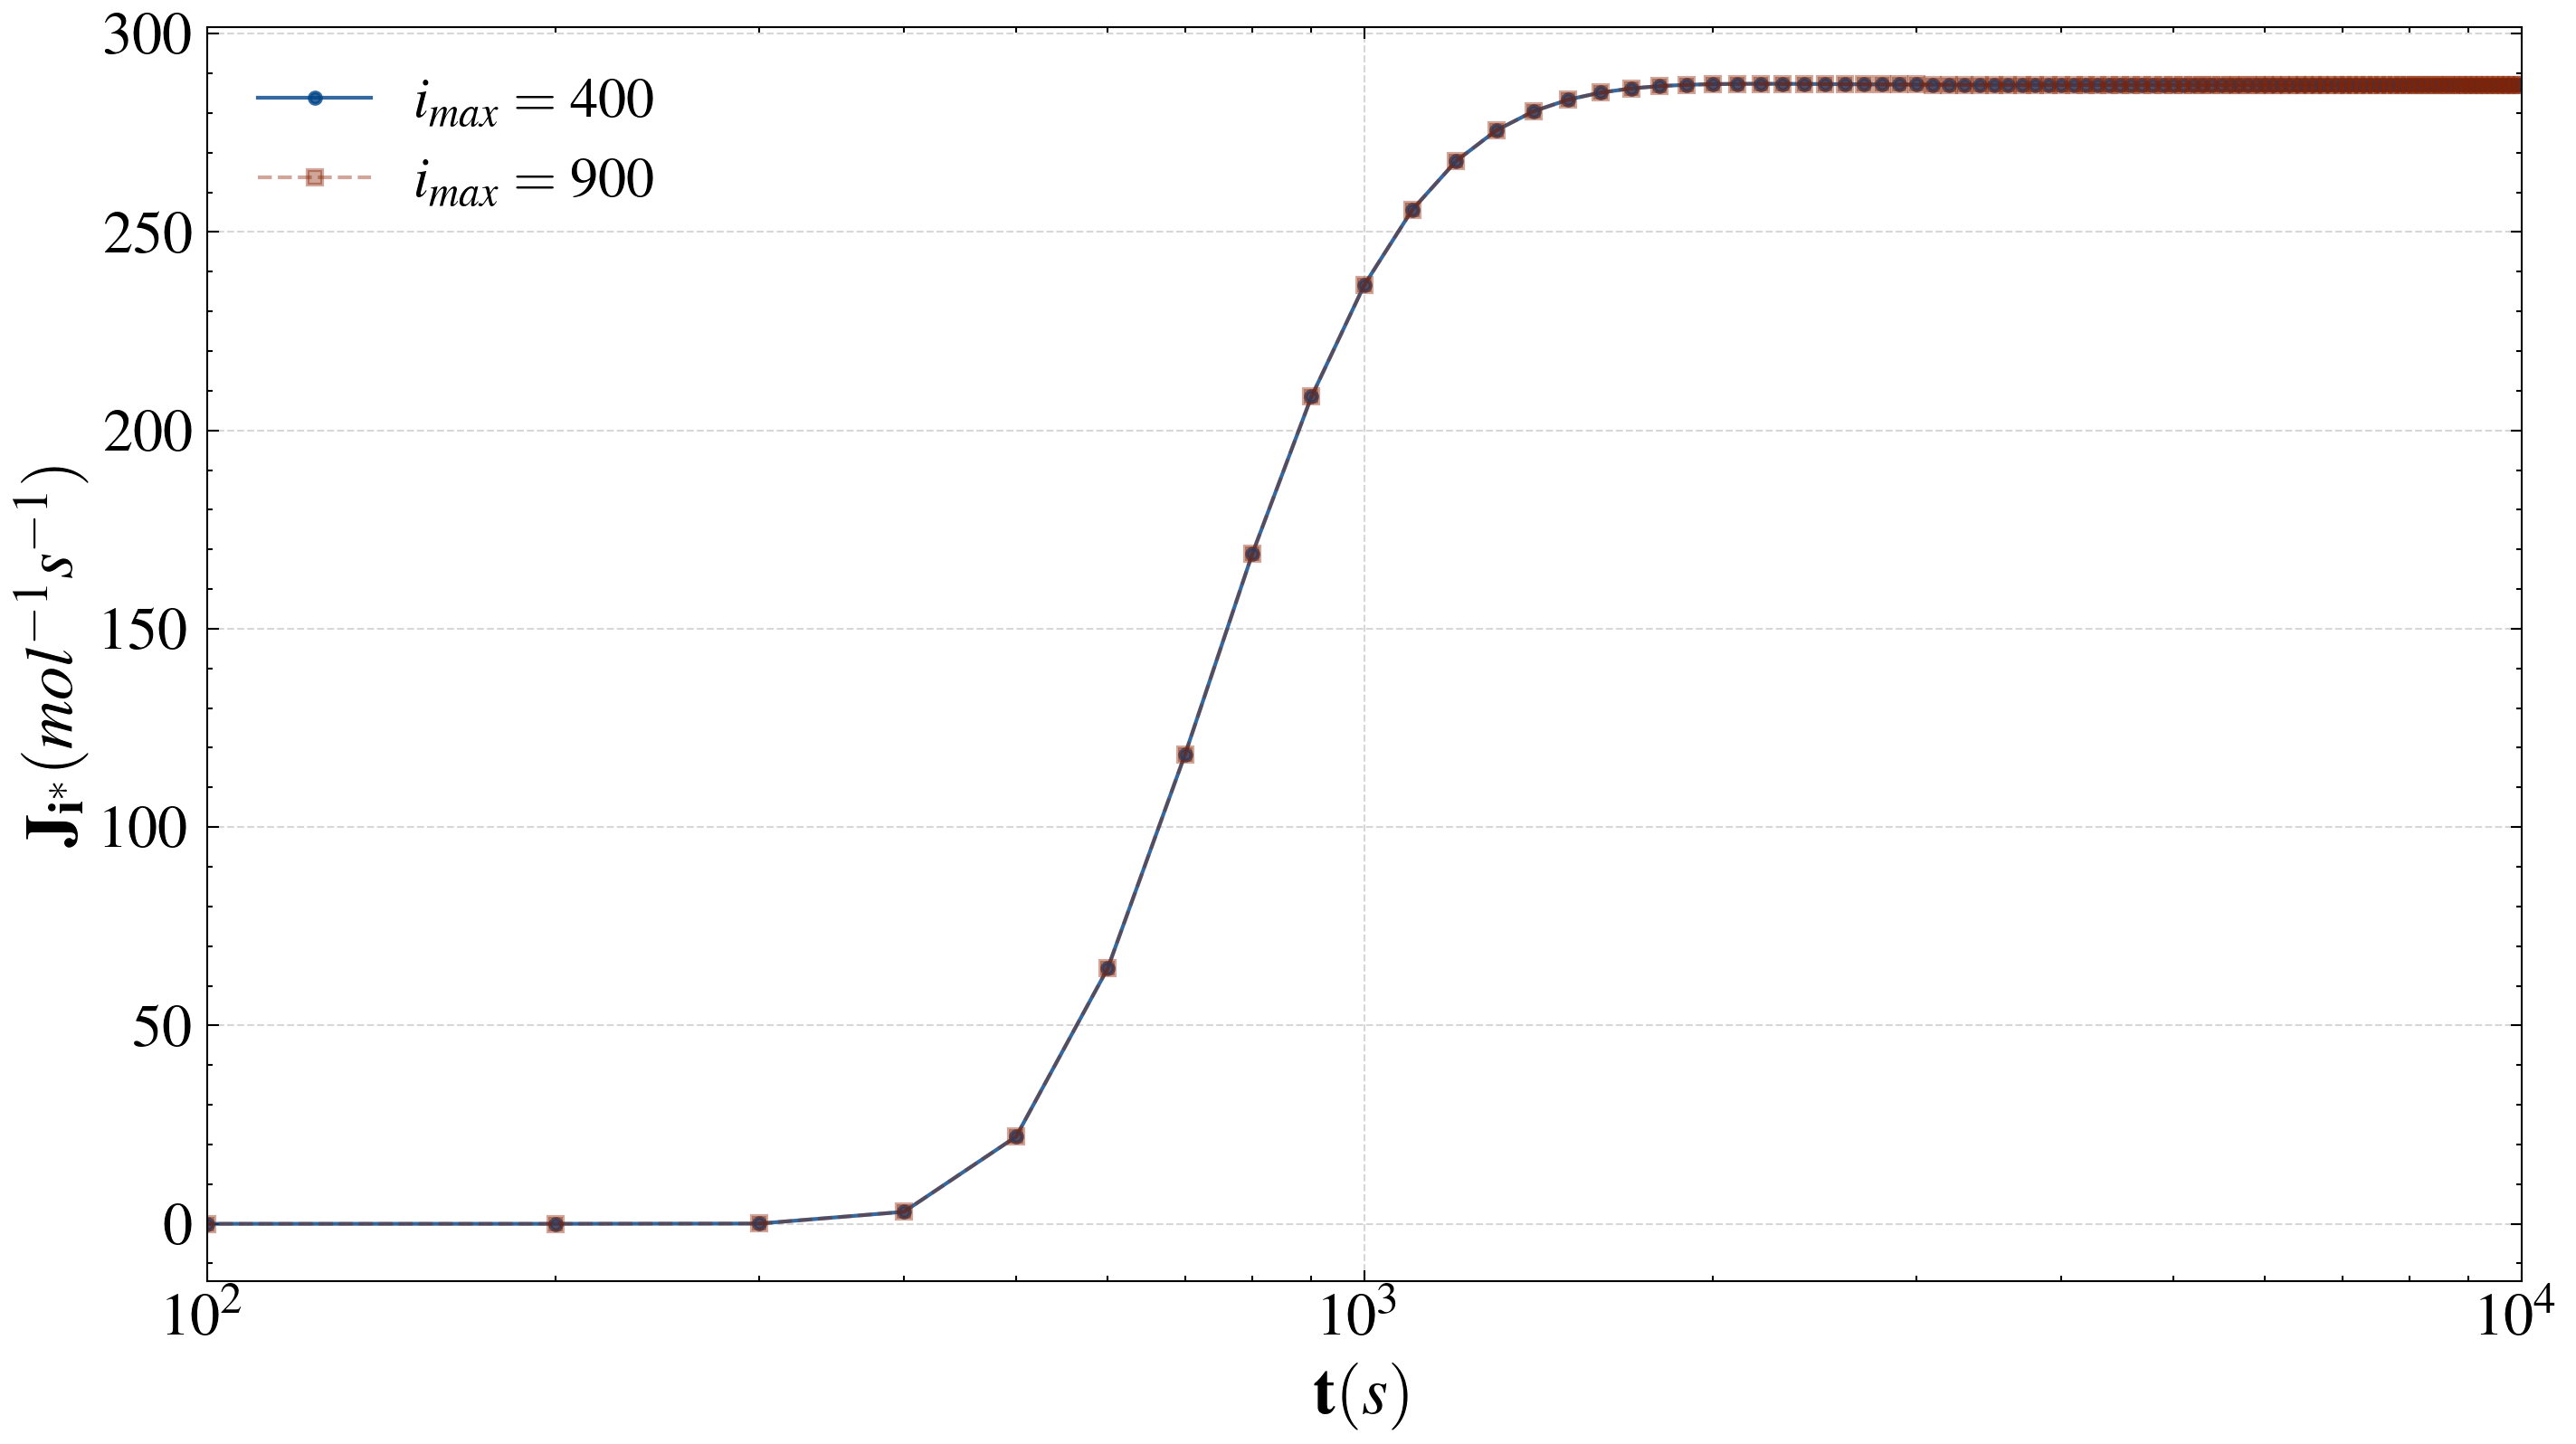
\includegraphics[width=1.1\linewidth]{postcritical_nucleation_rate_fe.png}
    \caption{Iron nucleation rates for different sizes $i_{\text{max}} = 400$ and $900$.}
    \label{fig:postcritical_nucleation_rate_fe}
\end{figure}

\begin{figure}[H]
    \centering
    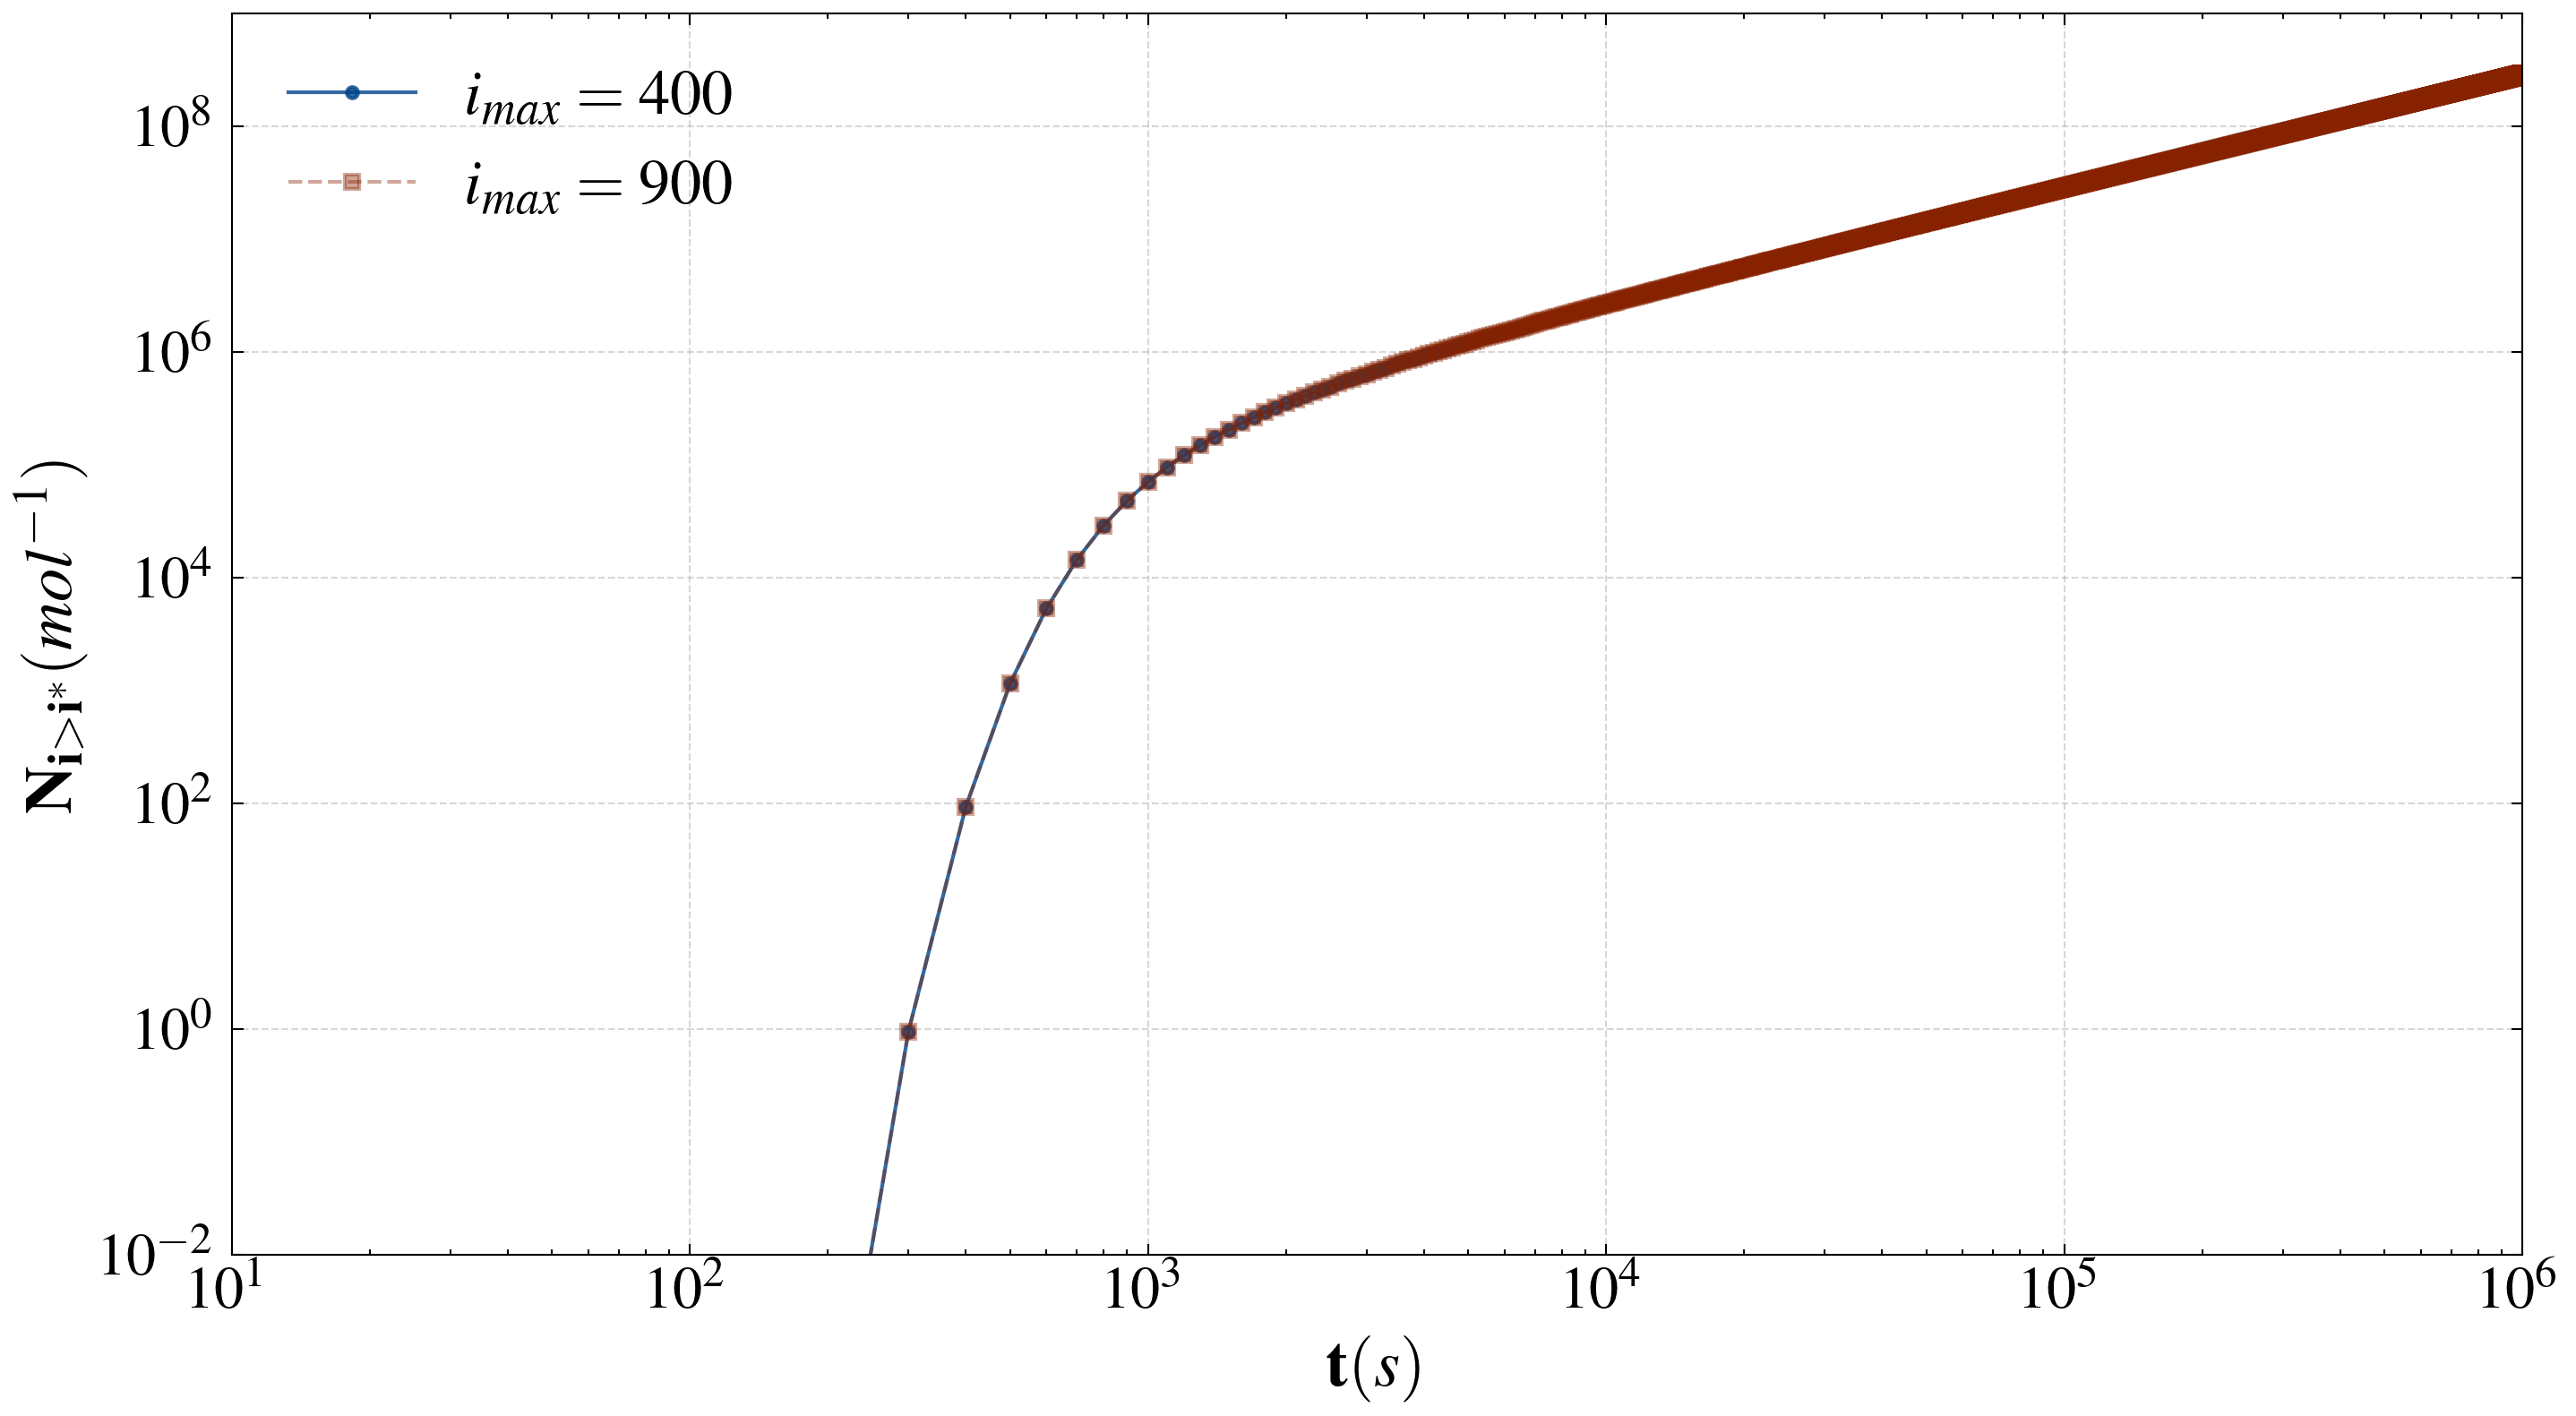
\includegraphics[width=1.1\linewidth]{postcritical_number_fe.png}
    \caption{Iron postcritical total number density for different sizes $i_{\text{max}} = 400$ and $900$.}
    \label{fig:postcritical_number_fe}
\end{figure}

\begin{figure}[H]
    \centering
    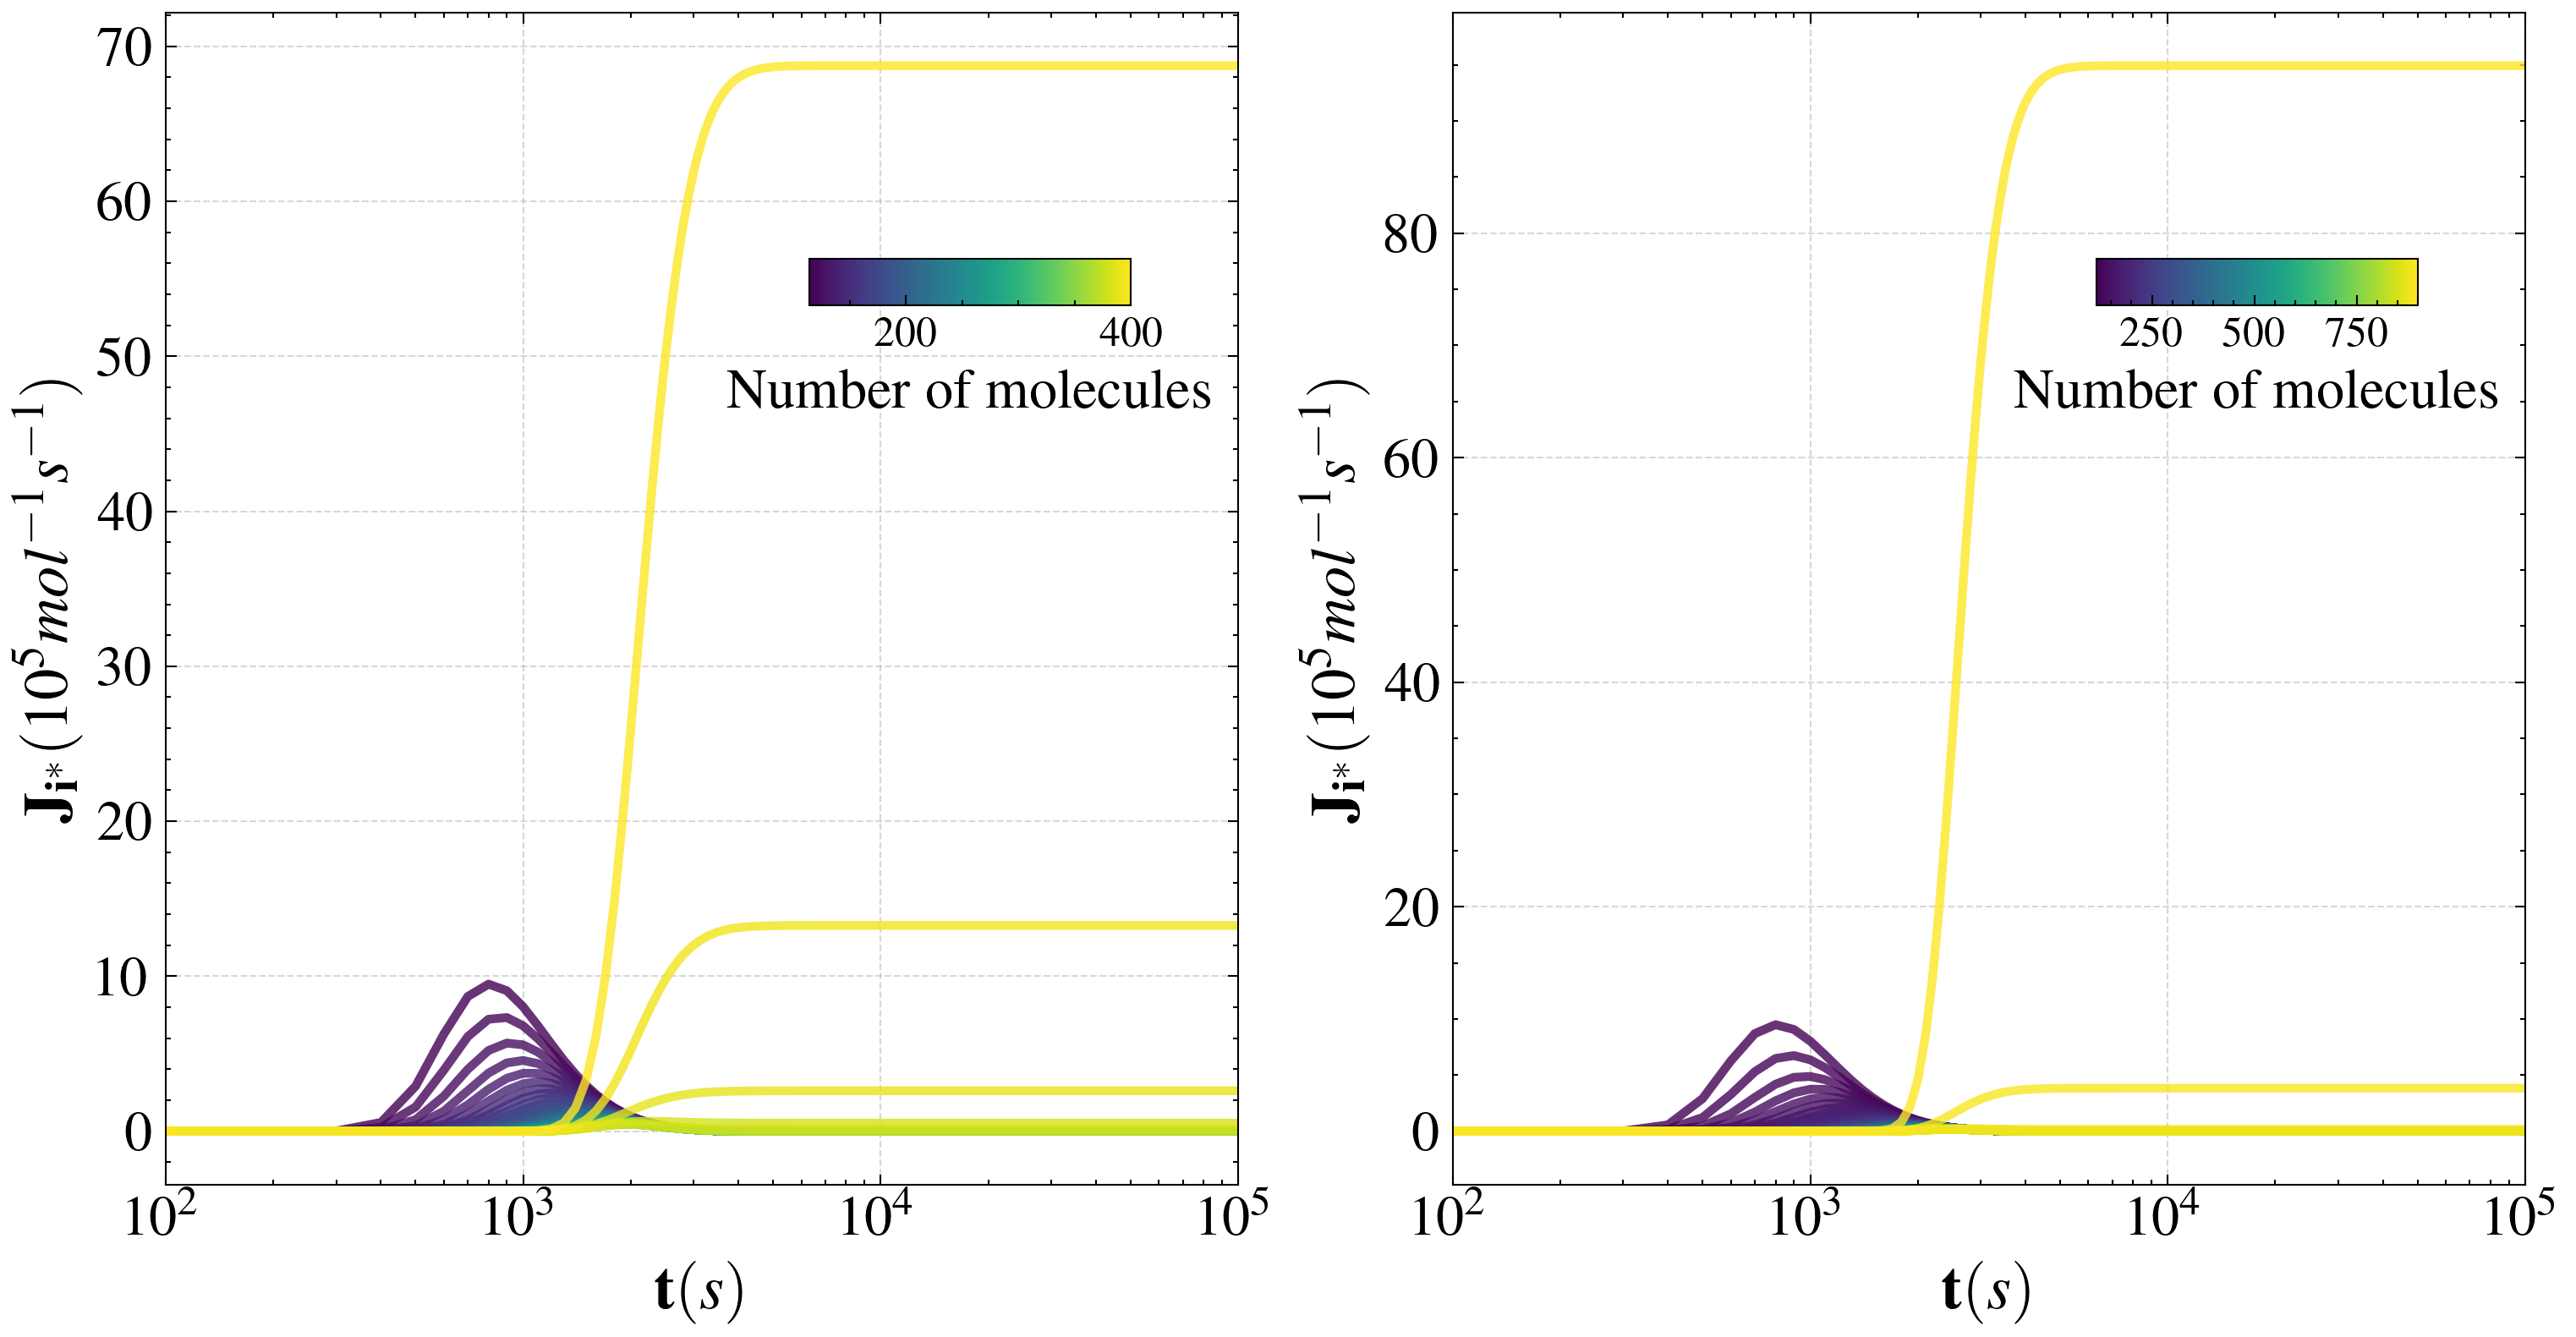
\includegraphics[width=1.1\linewidth]{postcritical_nucleation_rate_fe_particles_comparison.png}
    \caption{Iron nucleation rates for different observable sizes for $i_{\text{max}} = 400$ (left) and $900$ (right).}
    \label{fig:postcritical_nucleation_rate_fe_particles_comparison}
\end{figure}

\begin{figure}[H]
    \centering
    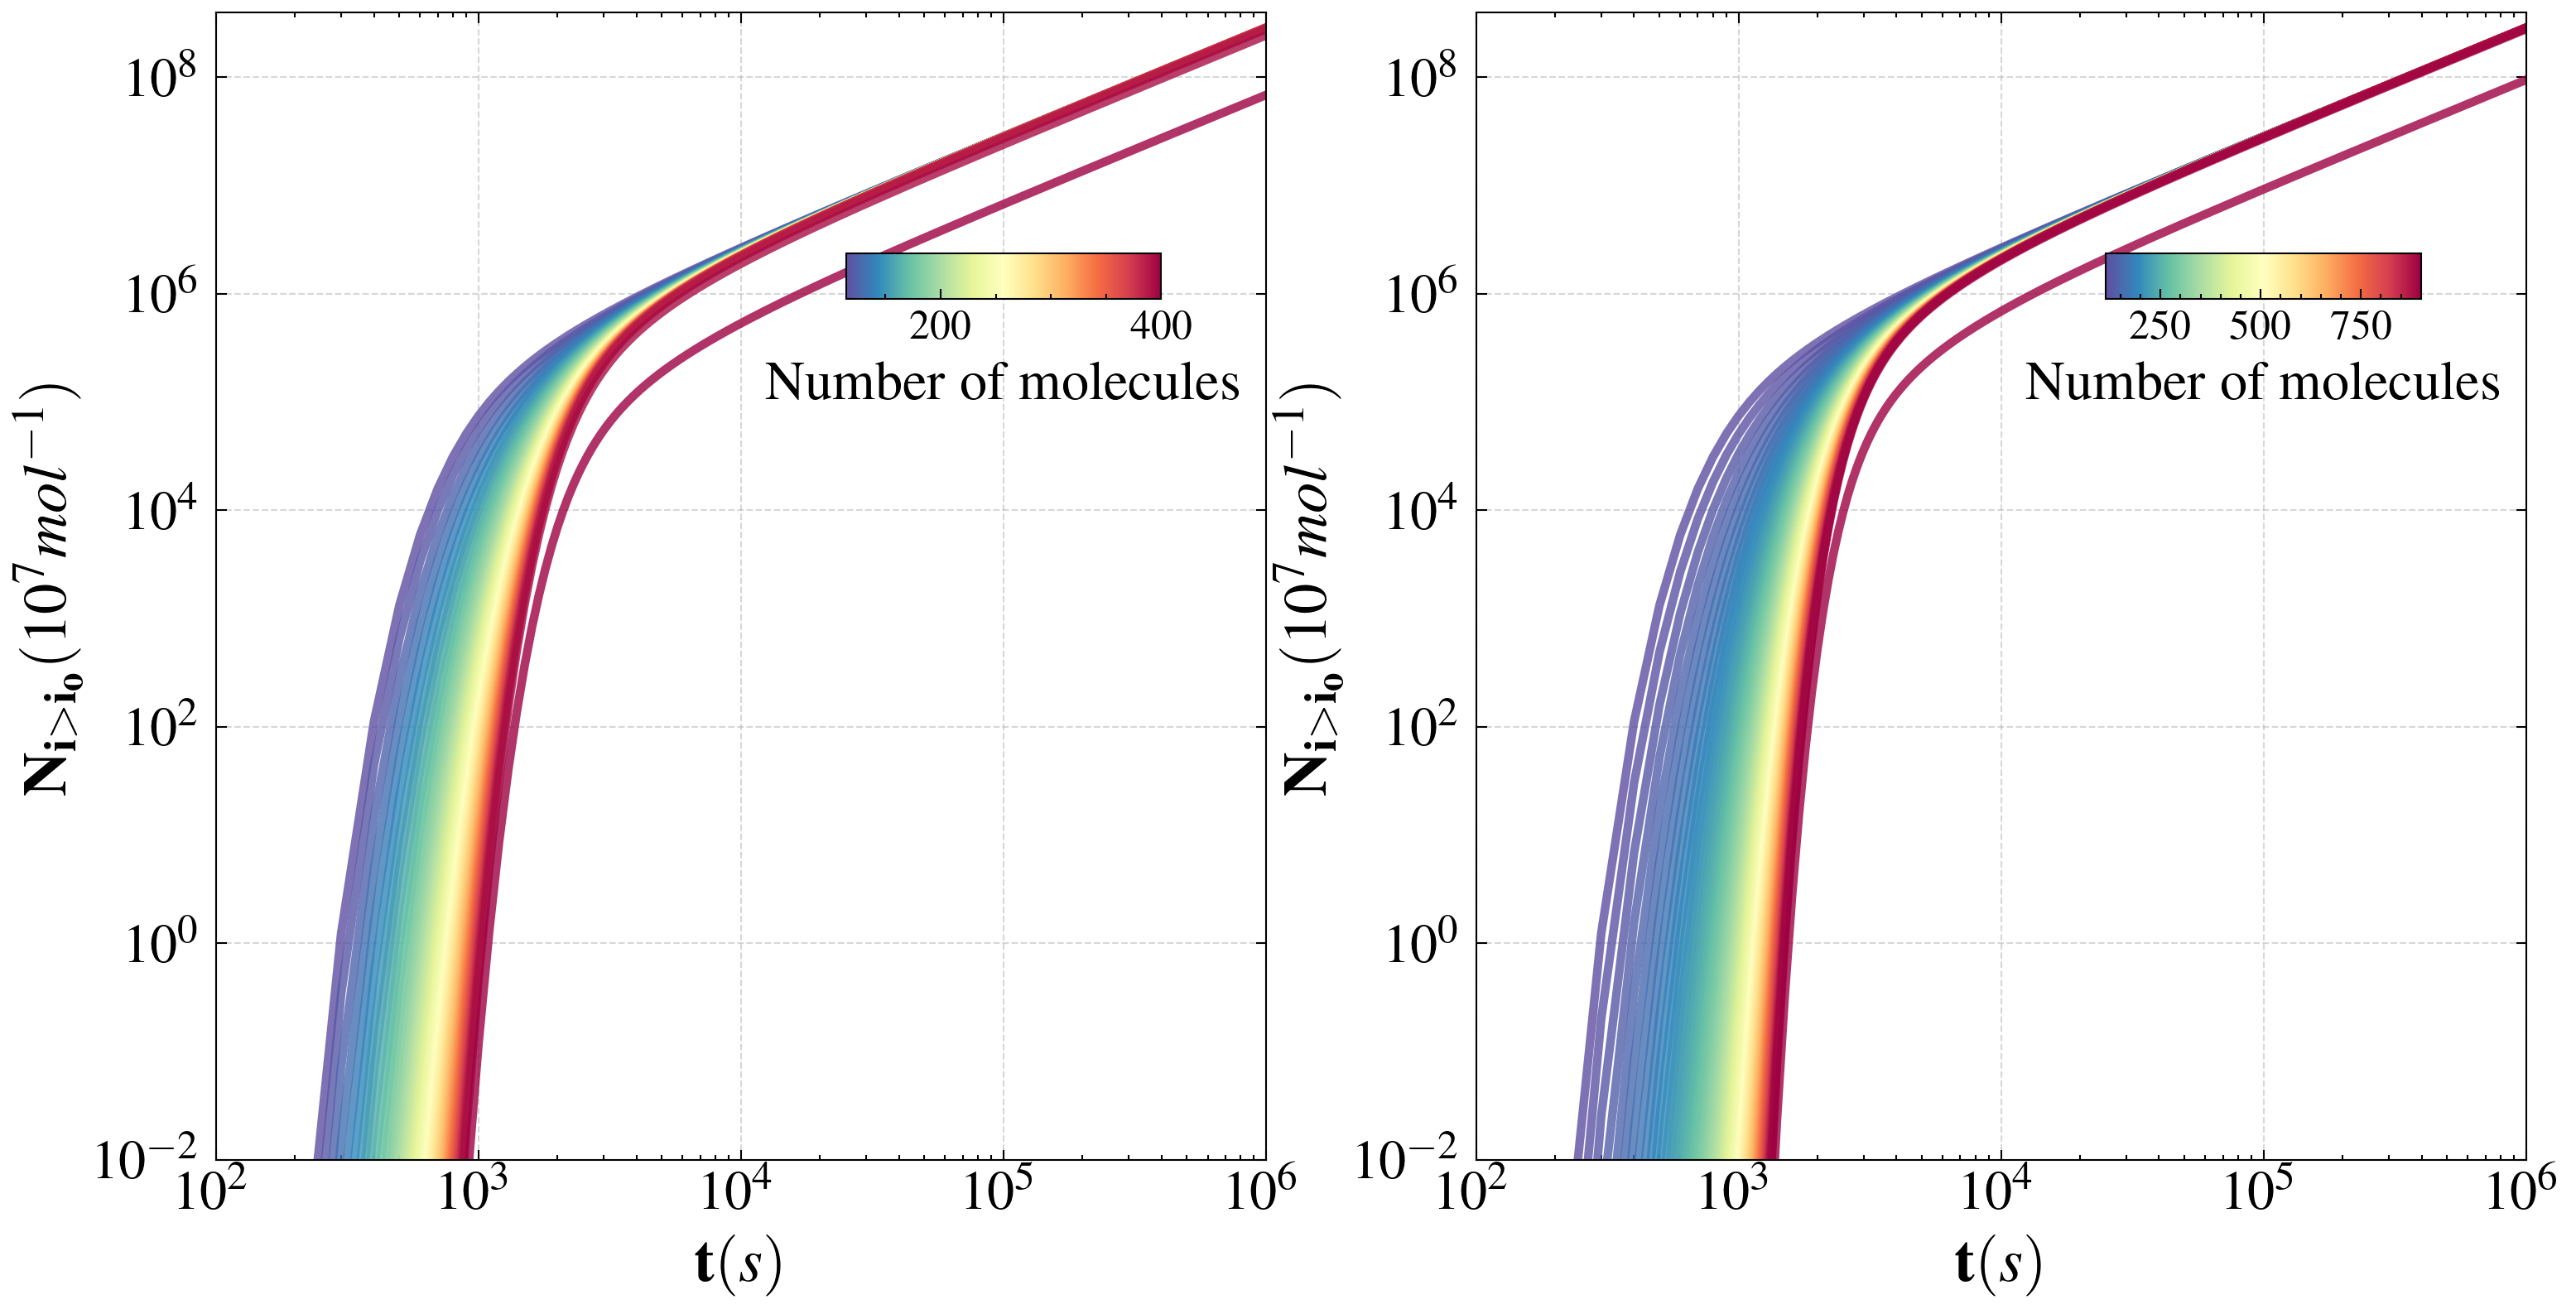
\includegraphics[width=1.1\linewidth]{postcritical_number_density_fe_particles_comparison.png}
    \caption{Iron postcritical total number density for different observable sizes for $i_{\text{max}} = 400$ (left) and $900$ (right).}
    \label{fig:postcritical_number_density_fe_particles_comparison}
\end{figure}


\paragraph{Cr}~\\
\vspace{1mm} % Adjust the space as needed

The phase diagram of the Li-Cr system is shown below.

\begin{figure}[H]
    \centering
    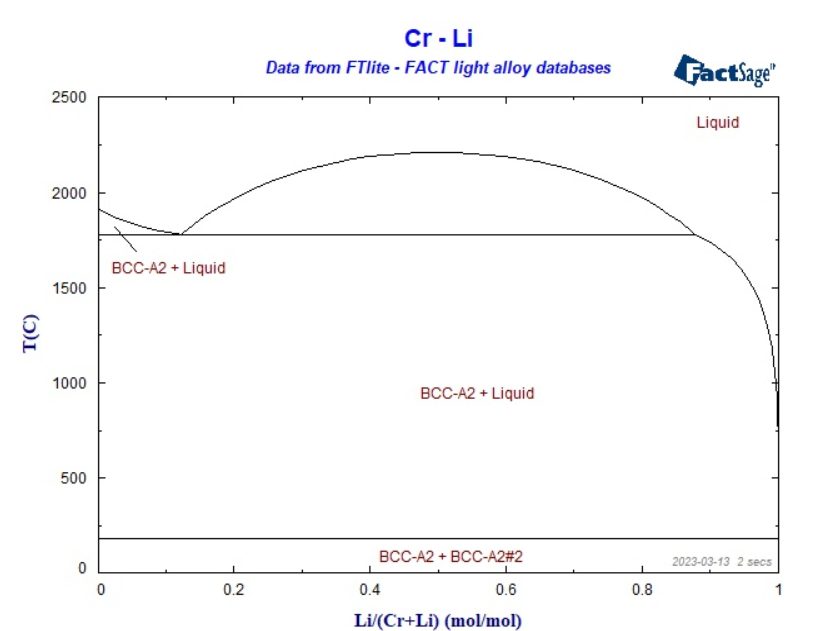
\includegraphics[width=0.9\linewidth]{Li_Cr_phase_diagram.png}
    \caption{Phase diagram of Li-Cr mixture from FactSage database \cite{Bale2016}.}
    \label{fig:cr_li_diagram}
\end{figure}

\begin{figure}[H]
    \centering
    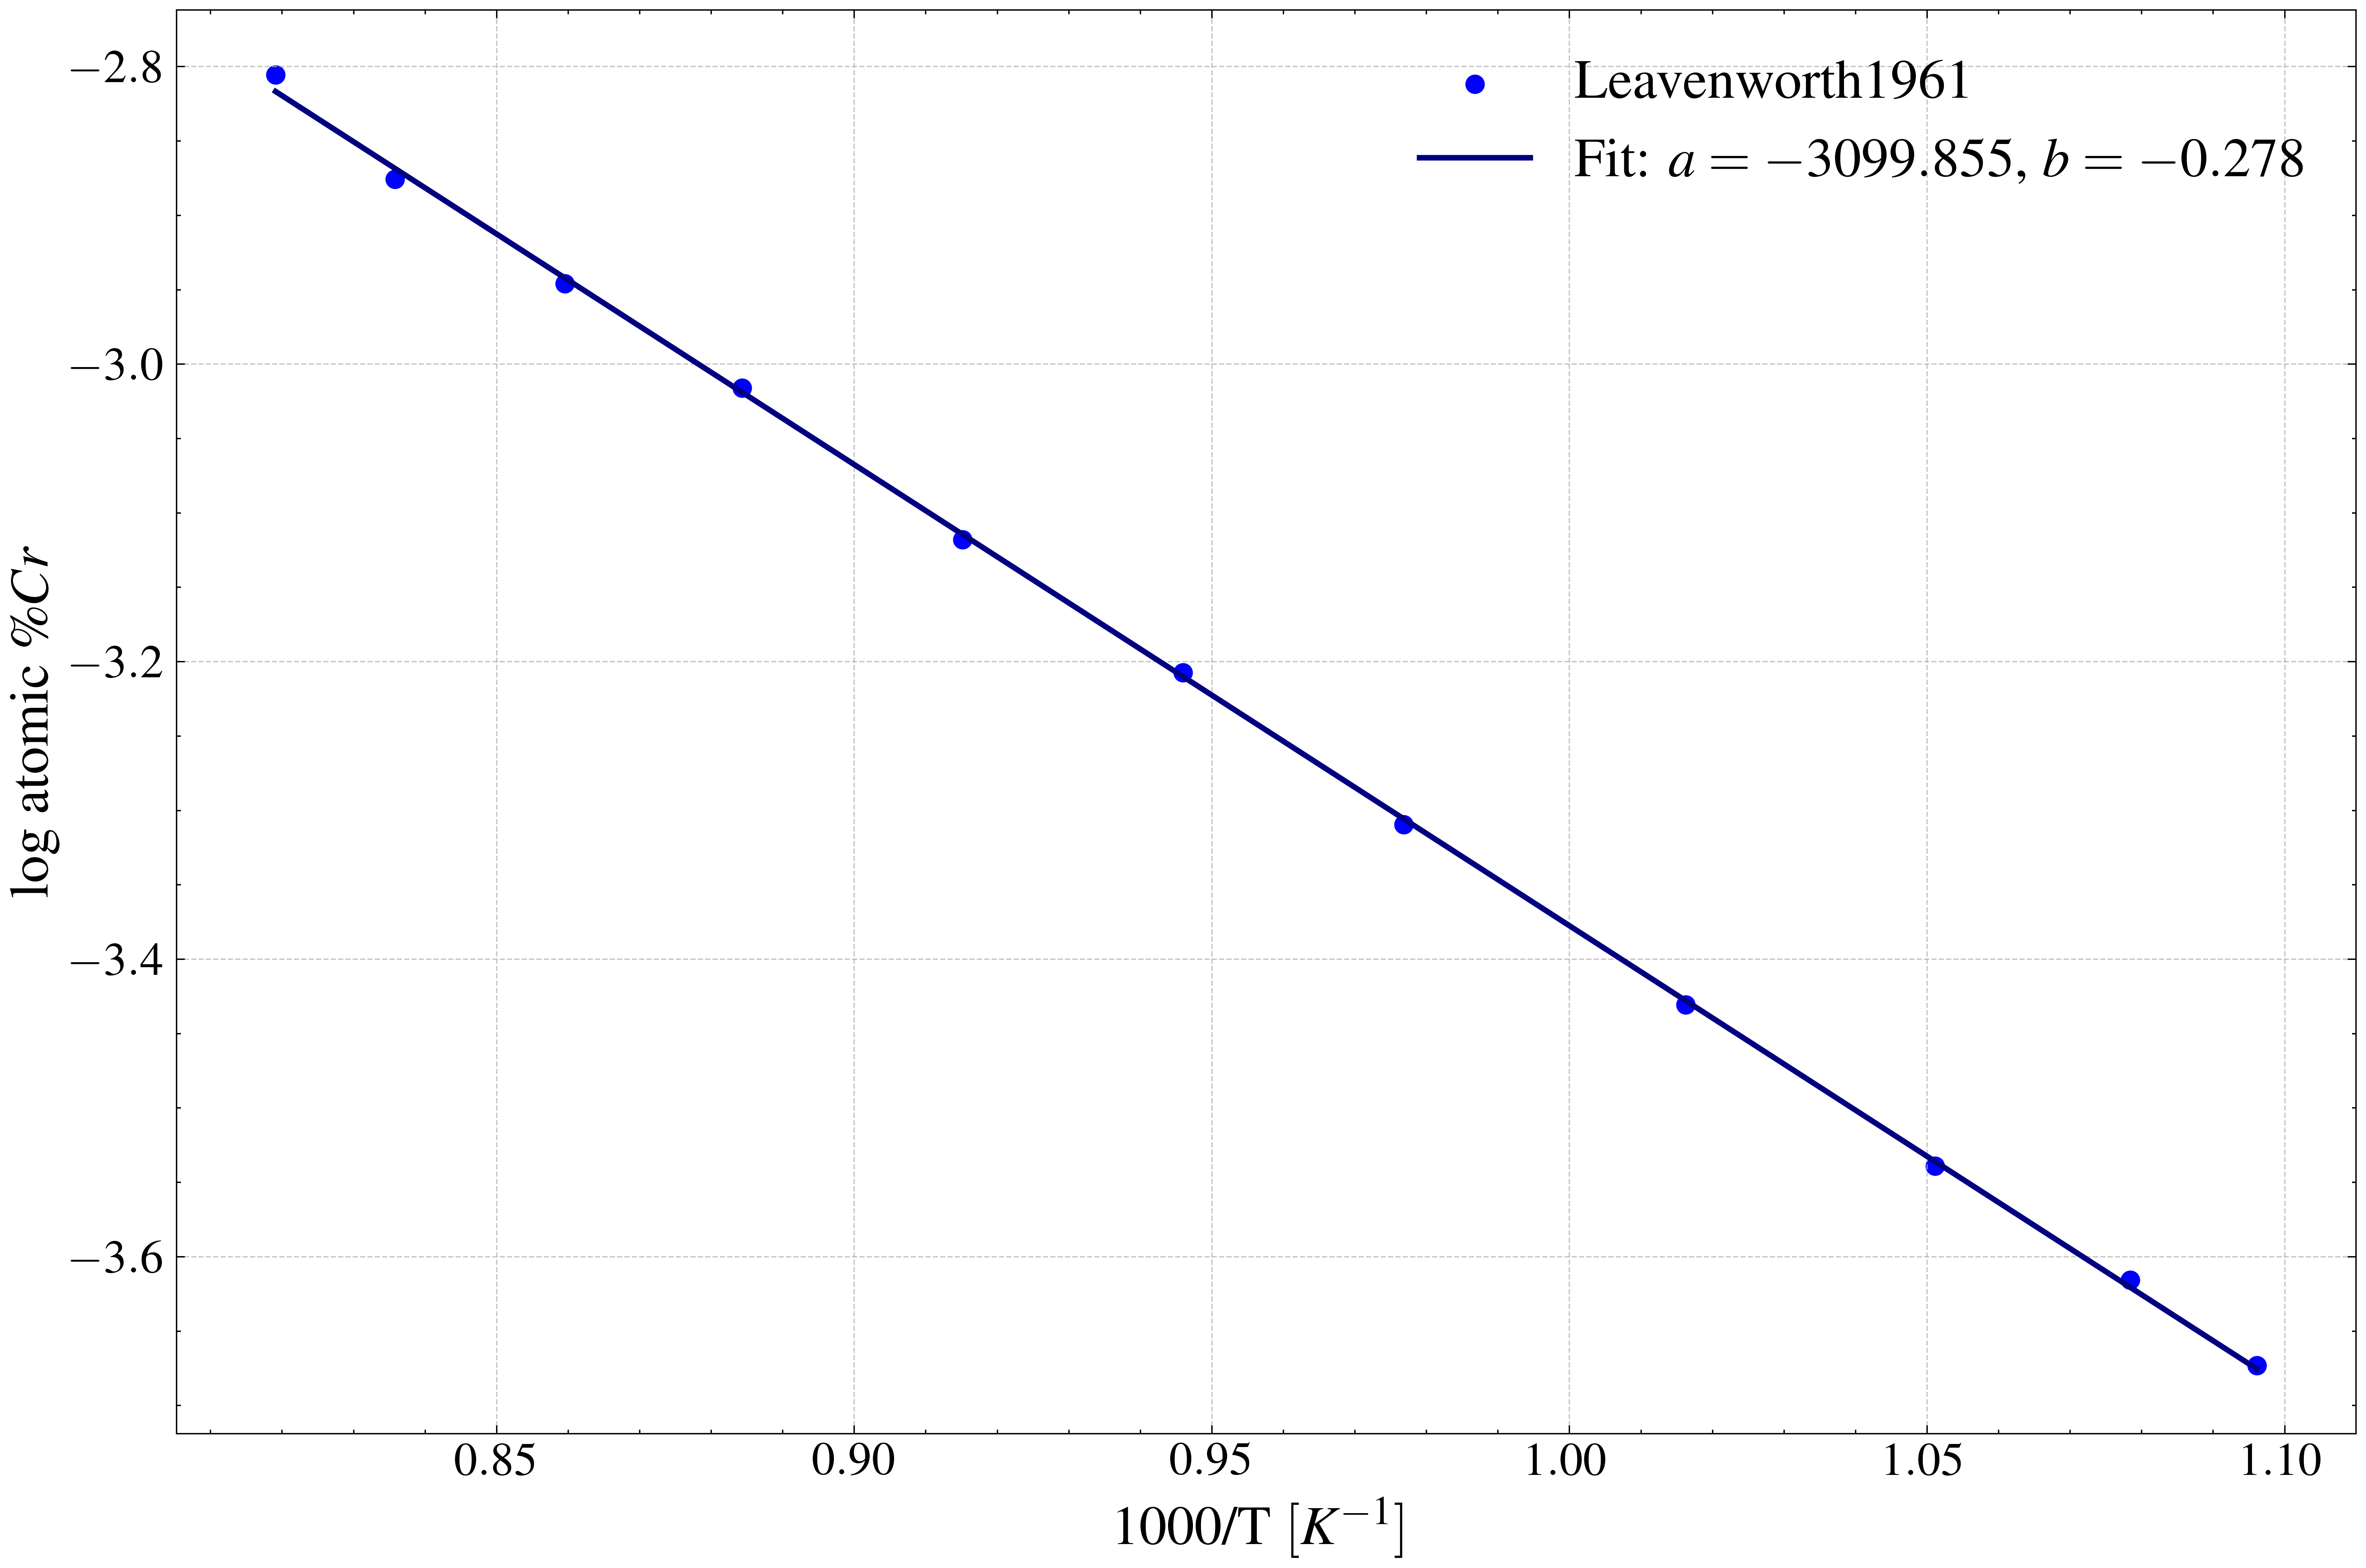
\includegraphics[width=0.9\linewidth]{solubility_cr.png}
    \caption{Cr solubility in liquid lithium dependence on temperature \ref{Leavenworth1961TheSO}.}
    \label{fig:solubility_cr}
\end{figure}


\begin{table}[ht]
	\centering
	\label{tab:your_label_here}
	\begin{tabular}{ccc}
	\hline
	$Reference$ & $x^{\text{A}}_{l,eq}$ & $x^{\text{A}}_{s,eq}$ \\ \hline
	FactSage \cite{Bale2016} & $5.86 \times 10^{-6} $        & $1.00$         \\
	Ref. \cite{Leavenworth1961TheSO}       & $1.21 \times 10^{-5}$         & -         \\
	\end{tabular}
	\caption{Equilibrium compositions of iron using FactSage and reference data.}
\end{table}

\begin{table}[ht]
	\centering
	\label{tab:molar_fractions_cr_li}
	\begin{tabular}{lccc}
	\hline
	\multicolumn{4}{c}{Molar fractions (T = 668 K)} \\
	\hline
	Species & Amount/mol & & \\
	\hline
	Cr & $2.0000 \times 10^{-8}$ & & \\
	Li & $1.0000 \times 10^{0}$ & & \\
	\hline
	\multicolumn{4}{c}{PHASE: Liquid\#1(\#2)} \\
	\hline
	Species & Amount/mol & Mole Fraction & Activity \\
	\hline
	Cr & $2.0000 \times 10^{-8}$ & $2.0000 \times 10^{-8}$ & $1.6853 \times 10^{-4}$ \\
	Li & $1.0000 \times 10^{0}$ & $1.0000 \times 10^{0}$ & $1.0000 \times 10^{0}$ \\
	Total & $1.0000 \times 10^{0}$ & $1.0000$ & $1.0000$ \\
	\hline
	\multicolumn{4}{c}{PHASE: BCC-A2\#1} \\
	\hline
	Species & Amount/mol & Mole Fraction & Activity \\
	\hline
	Cr & $0.0000 \times 10^{0}$ & $6.7643 \times 10^{-13}$ & $3.4140 \times 10^{-3}$ \\
	Li & $0.0000 \times 10^{0}$ & $1.0000$ & $7.7430 \times 10^{-1}$ \\
	Total & $0.0000 \times 10^{0}$ & $1.0000$ & $7.7430 \times 10^{-1}$ \\
	\hline
	\end{tabular}
	\caption{Equilibrium compositions of chromium using FactSage with a chromium molar fraction used as input.}
\end{table}

\begin{table}[ht]
	\centering
	\label{tab:molar_fractions_cr_li_updated}
	\begin{tabular}{lccc}
	\hline
	\multicolumn{4}{c}{Molar fractions (T = 668 K)} \\
	\hline
	Species & Amount/mol & & \\
	\hline
	Cr & $1.1190 \times 10^{-5}$ & & \\
	Li & $9.9999 \times 10^{-1}$ & & \\
	\hline
	\multicolumn{4}{c}{PHASE: Liquid\#1} \\
	\hline
	Species & Amount/mol & Mole Fraction & Activity \\
	\hline
	Cr & $5.8621 \times 10^{-6}$ & $5.8622 \times 10^{-6}$ & $4.9364 \times 10^{-2}$ \\
	Li & $9.9999 \times 10^{-1}$ & $9.9999 \times 10^{-1}$ & $9.9999 \times 10^{-1}$ \\
	Total & $9.9999 \times 10^{-1}$ & $1.0000$ & $1.0000$ \\
	\hline
	\multicolumn{4}{c}{PHASE: BCC-A2\#1} \\
	\hline
	Species & Amount/mol & Mole Fraction & Activity \\
	\hline
	Cr & $5.3279 \times 10^{-6}$ & $1.0000$ & $1.0000$ \\
	Li & $6.3285 \times 10^{-16}$ & $1.1878 \times 10^{-10}$ & $7.7430 \times 10^{-1}$ \\
	Total & $5.3279 \times 10^{-6}$ & $1.0000$ & $1.0000$ \\
	\hline
	\end{tabular}
	\caption{Equilibrium compositions of chromium using FactSage with a chromium molar fraction increased to $x^{\text{A}}_{l} = 1.1190 \times 10^{-5}$.}
\end{table}


\begin{table}[h]
    \centering
    \begin{tabular}{|l|l|l|}
    \hline
    \textbf{Parameter} & \textbf{Symbol} & \textbf{Value (Unit)} \\ \hline
    Temperature        & $T$             & 668 K                 \\ \hline
    Molar Mass         & $M$             & 51.99 g/mol         \\ \hline
    Mass Density       & $\rho$          & 7.19 g/cm$^3$         \\ \hline
    Melting Point      & $T_m$           & 2130 K                \\ \hline
    Heat of Fusion     & $\Delta H_f$    & 20.48 kJ/mol           \\ \hline
    Surface Tension    & $\sigma$        & 0.14 J/m$^2$          \\ \hline
	Diffusion Coefficient & $D$          & $8 \times 10^{-11}$ m$^2$/s \\ \hline
    \end{tabular}
    \caption{Parameters for Cr}
    \label{tab:params_Fe}
\end{table}

In Table. \ref{tab:critical_cr} the critical parameters are obtained.
\begin{table}[h]
	\centering
	\begin{tabular}{|l|l|l|}
	\hline
	\textbf{Parameter} & \textbf{Symbol} & \textbf{Value (Unit)} \\ \hline
	Critical radius        & $r^*$             & 0.45 nm                 \\ \hline
	Energy barrier         & $\Delta G^*$             & $2.26 \times 10^{-19}$ J         \\ \hline
	Critical number of molecules       & $n^*$          & 31         \\ \hline
	\end{tabular}
	\caption{Critical values for Cr}
	\label{tab:critical_cr}
\end{table}


\begin{figure}[H]
    \centering
    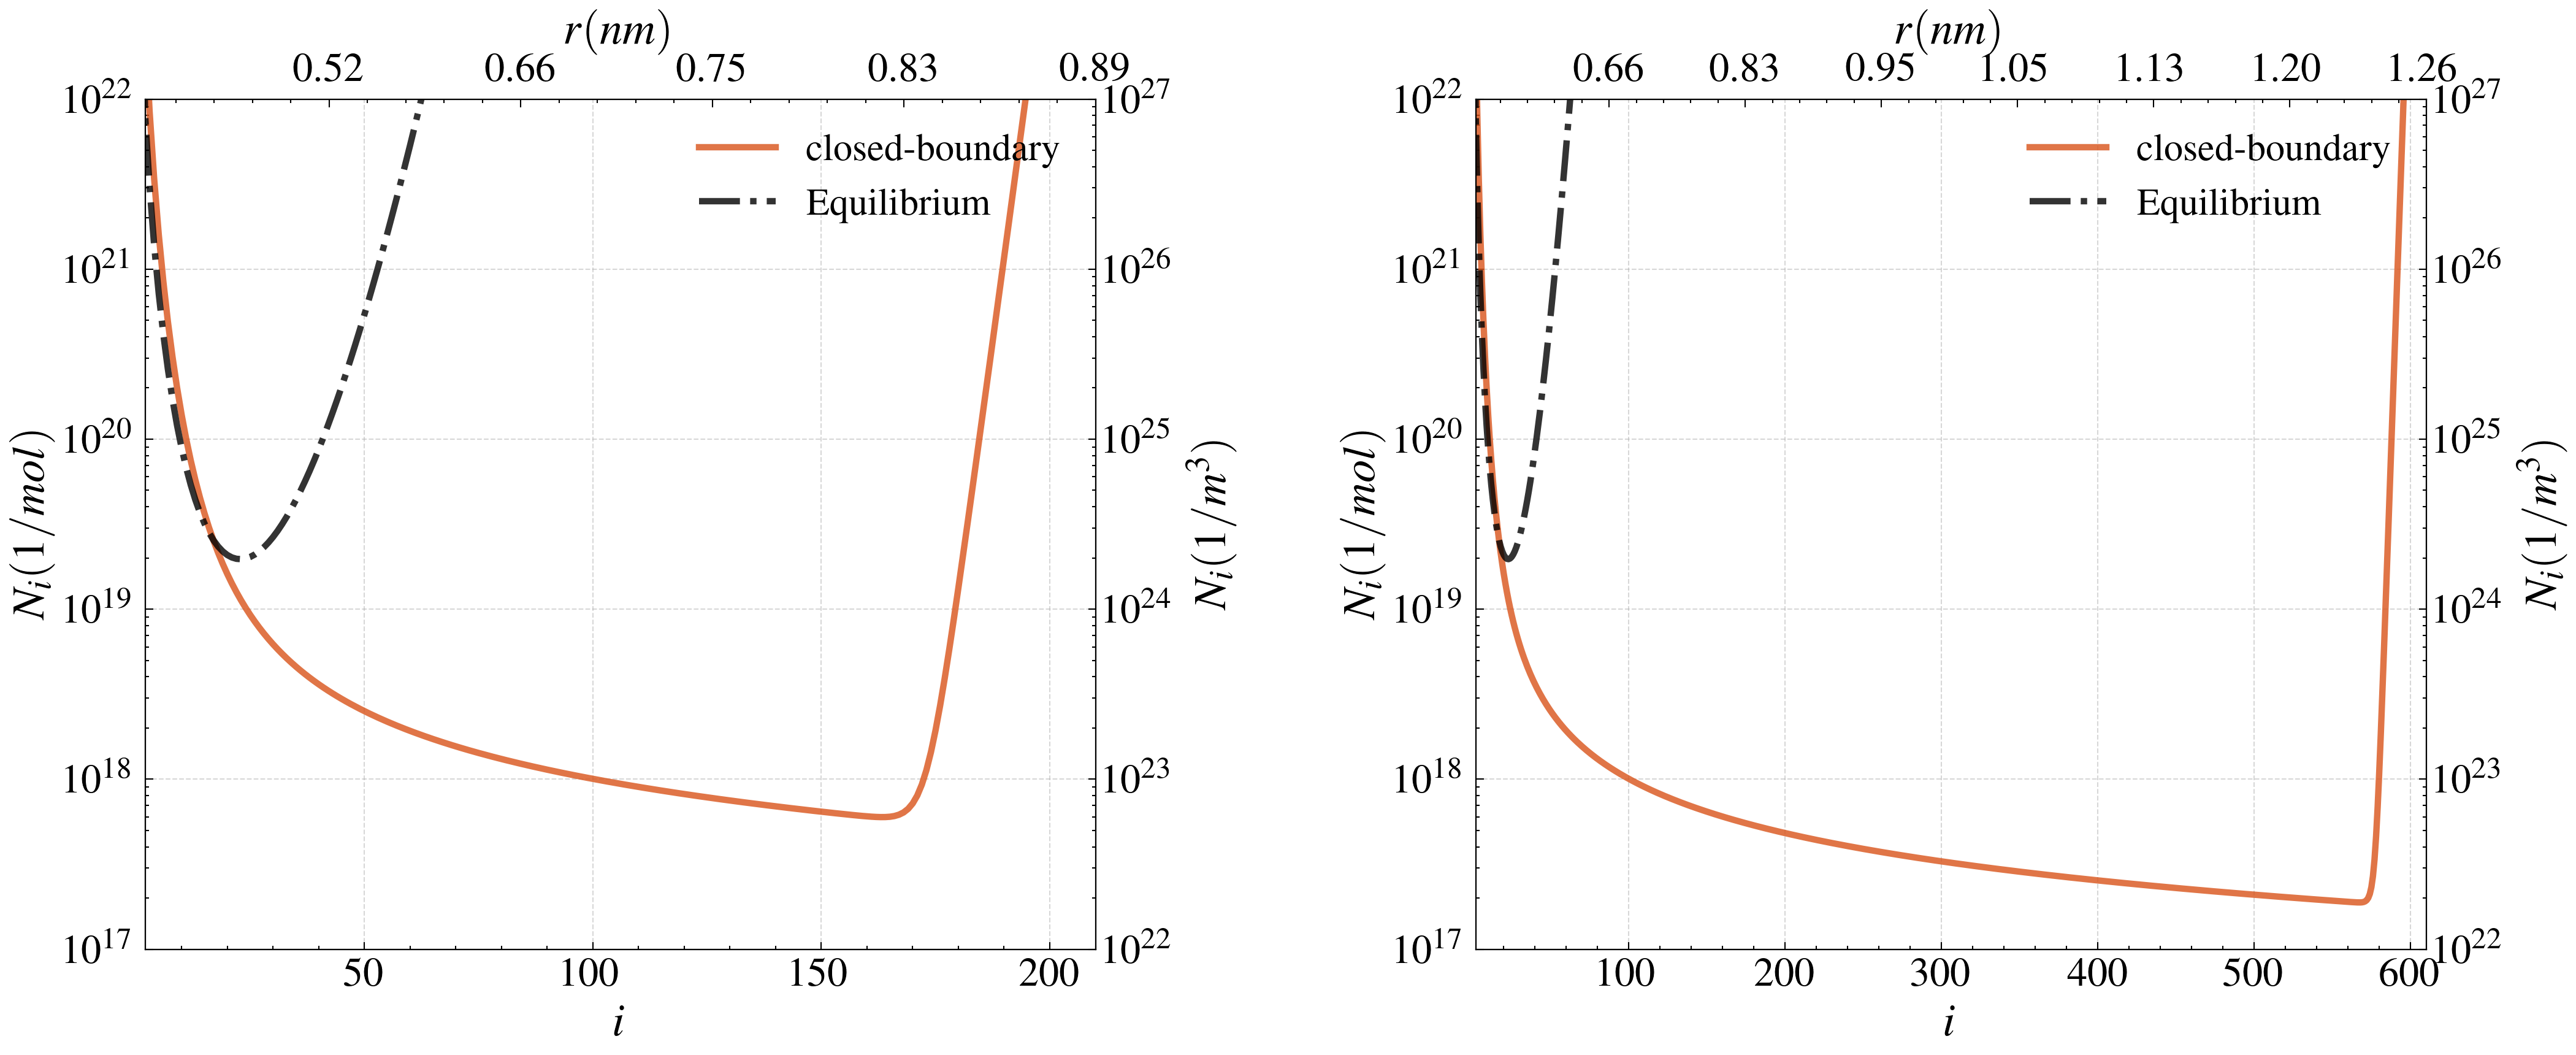
\includegraphics[width=1.1\linewidth]{psd_cr.png}
    \caption{Iron cluster number density distribution for different sizes $i_{\text{max}} = 200$ and $600$.}
    \label{fig:psd_iron}
\end{figure}

\begin{figure}[H]
    \centering
    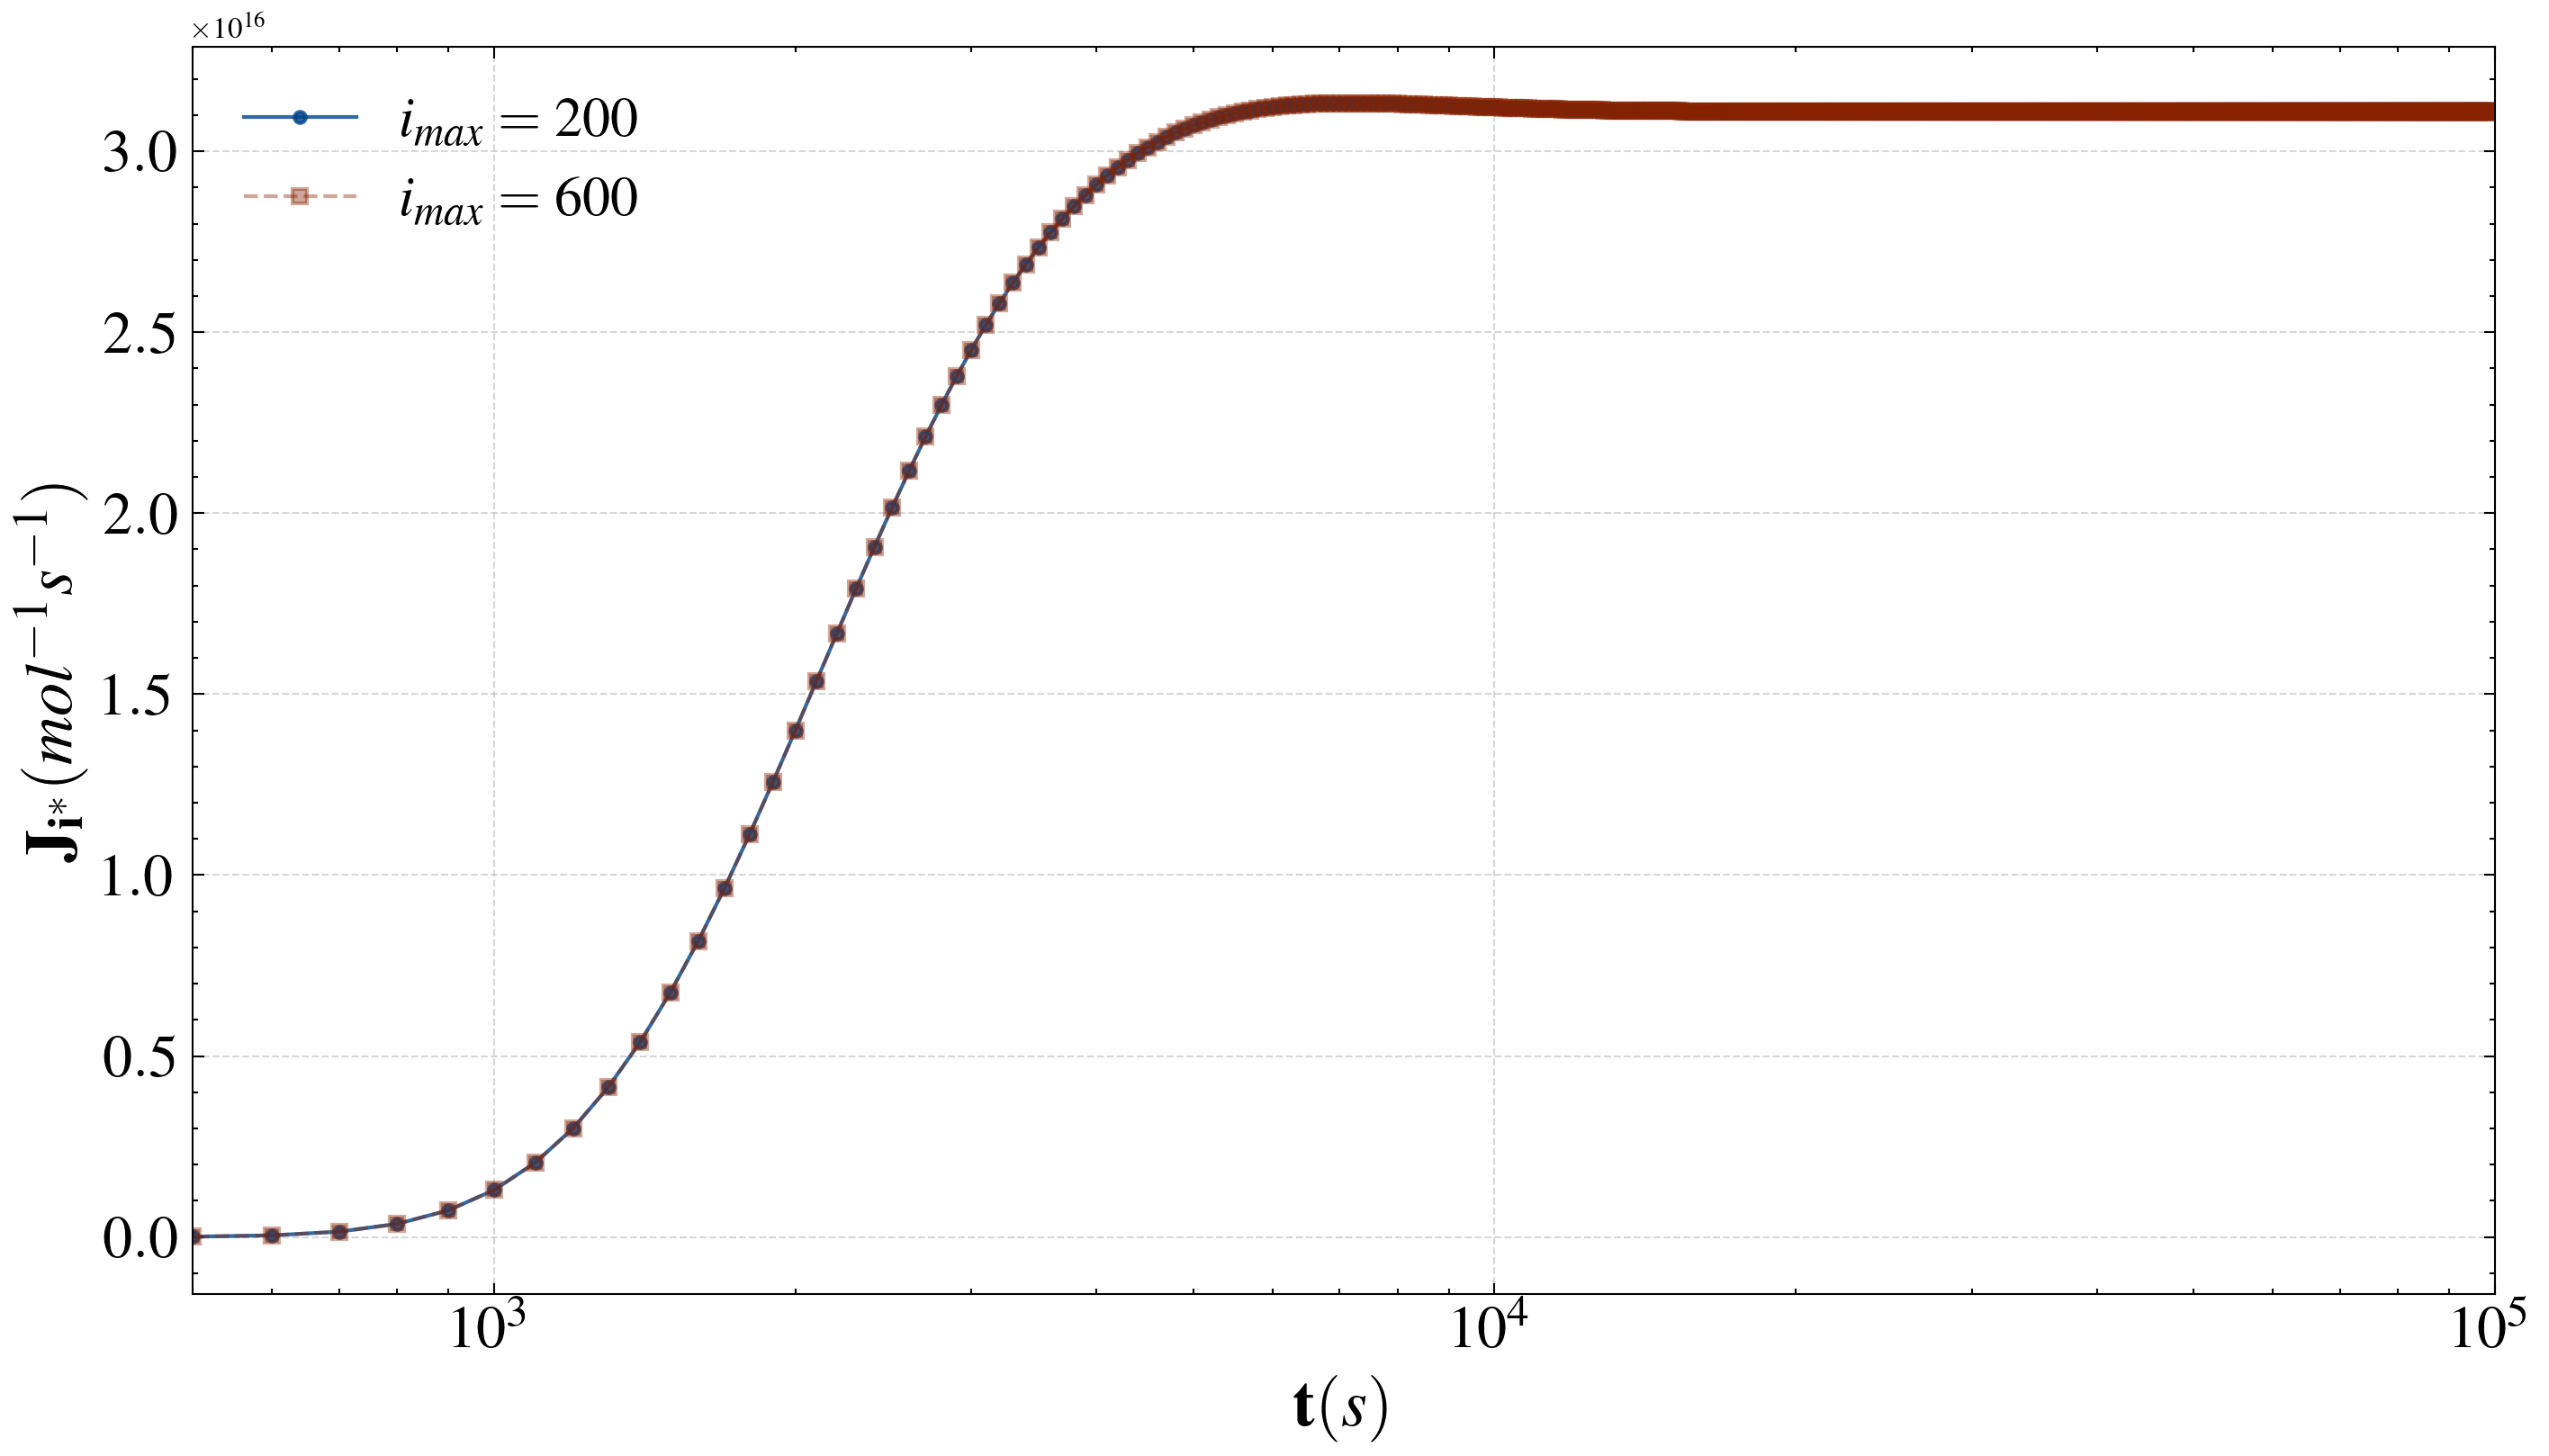
\includegraphics[width=1.1\linewidth]{postcritical_nucleation_rate_cr.png}
    \caption{Iron nucleation rates for different sizes $i_{\text{max}} = 400$ and $900$.}
    \label{fig:postcritical_nucleation_rate_fe}
\end{figure}

\begin{figure}[H]
    \centering
    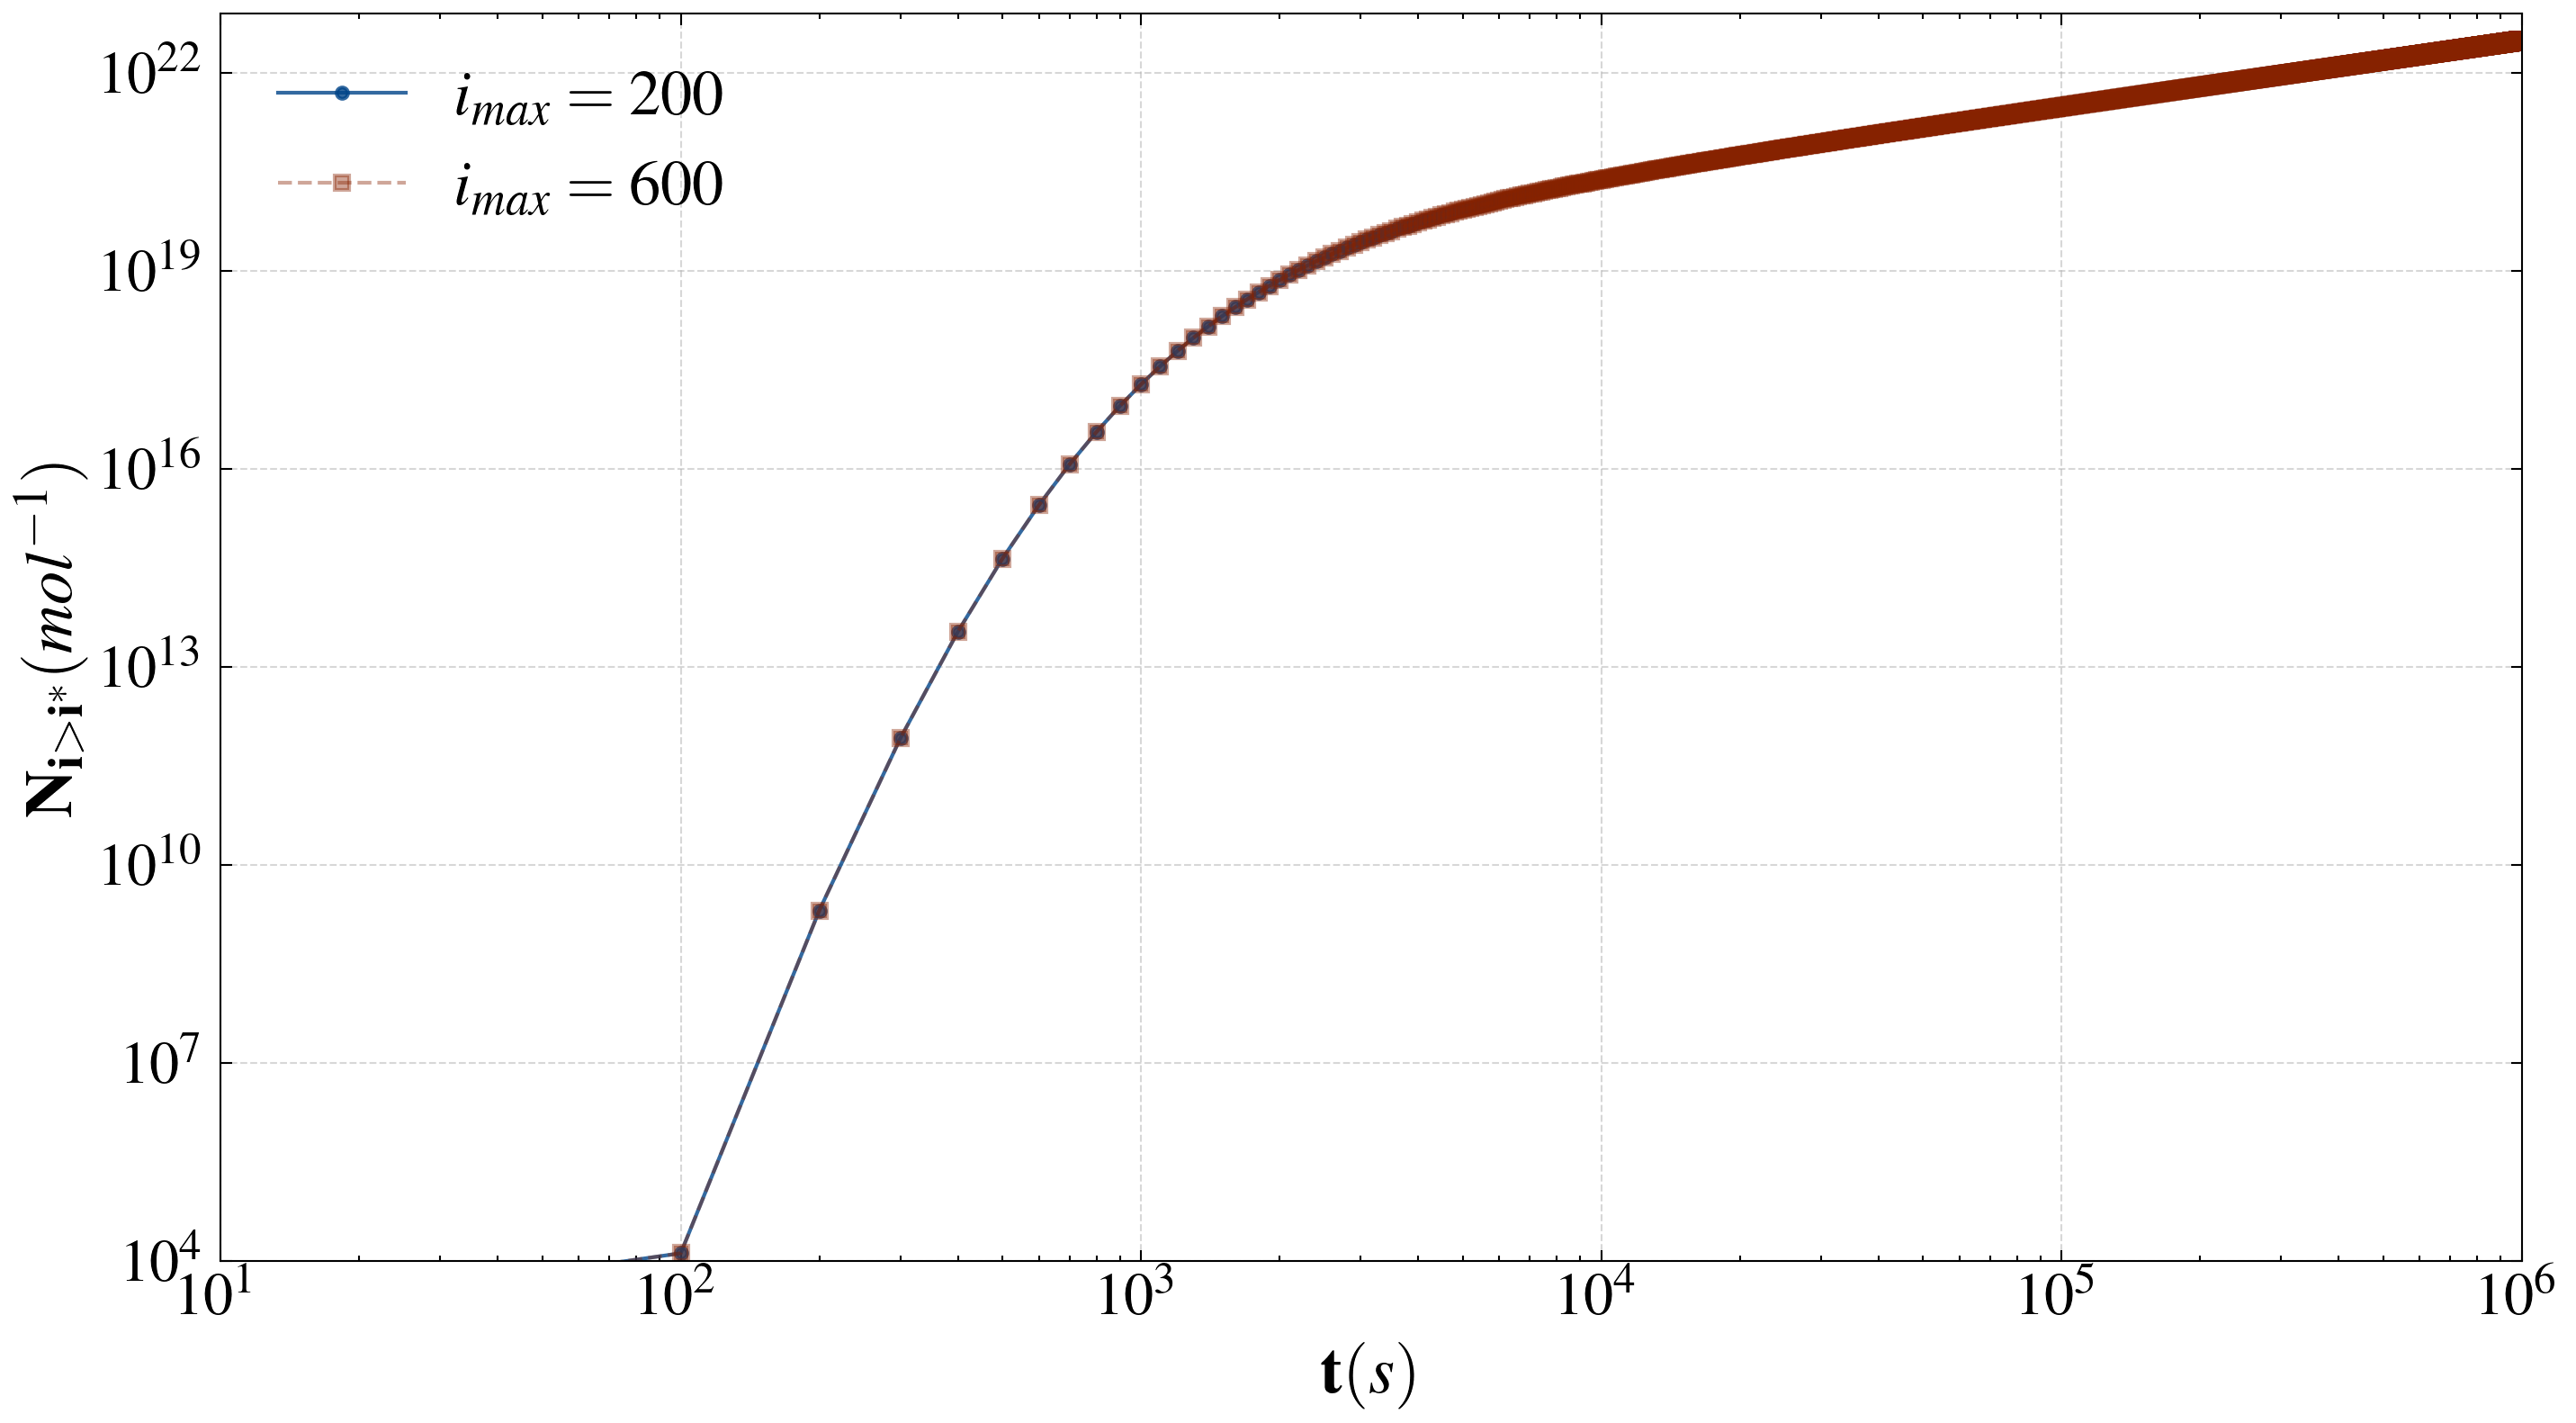
\includegraphics[width=1.1\linewidth]{postcritical_number_cr.png}
    \caption{Iron postcritical total number density for different sizes $i_{\text{max}} = 200$ and $600$.}
    \label{fig:postcritical_number_fe}
\end{figure}

\begin{figure}[H]
    \centering
    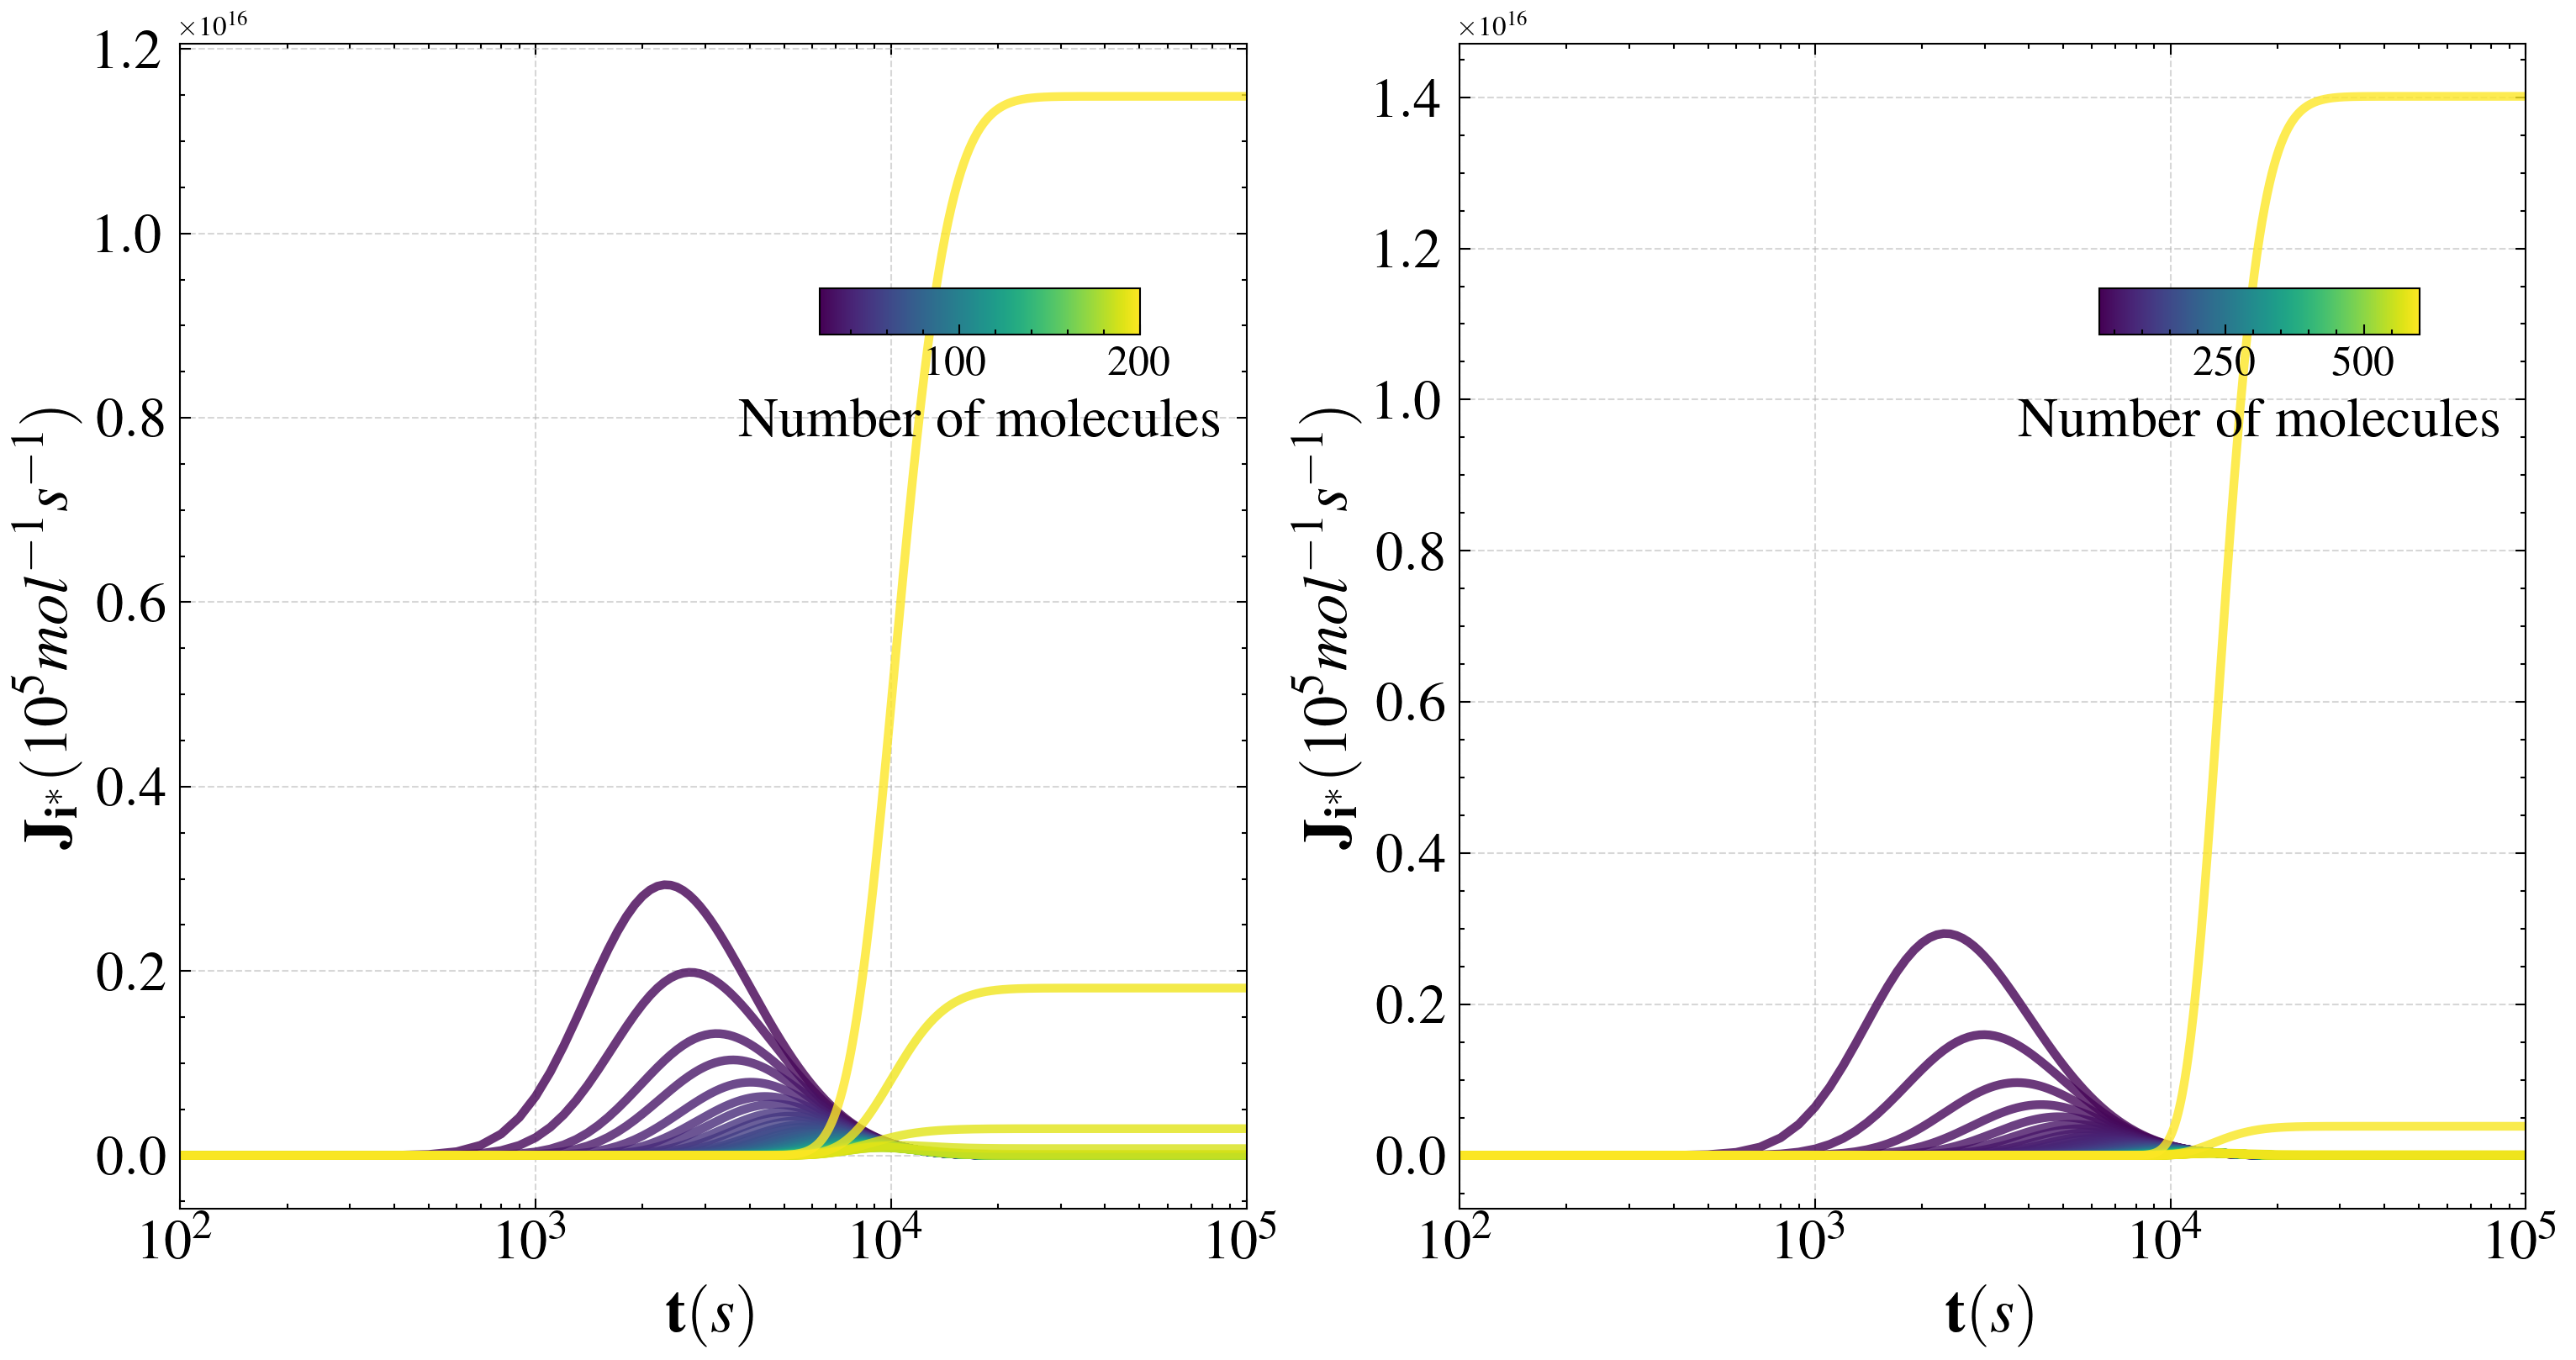
\includegraphics[width=1.1\linewidth]{postcritical_nucleation_rate_cr_particles_comparison.png}
    \caption{Iron nucleation rates for different observable sizes for $i_{\text{max}} = 200$ (left) and $600$ (right).}
    \label{fig:postcritical_nucleation_rate_fe_particles_comparison}
\end{figure}

\begin{figure}[H]
    \centering
    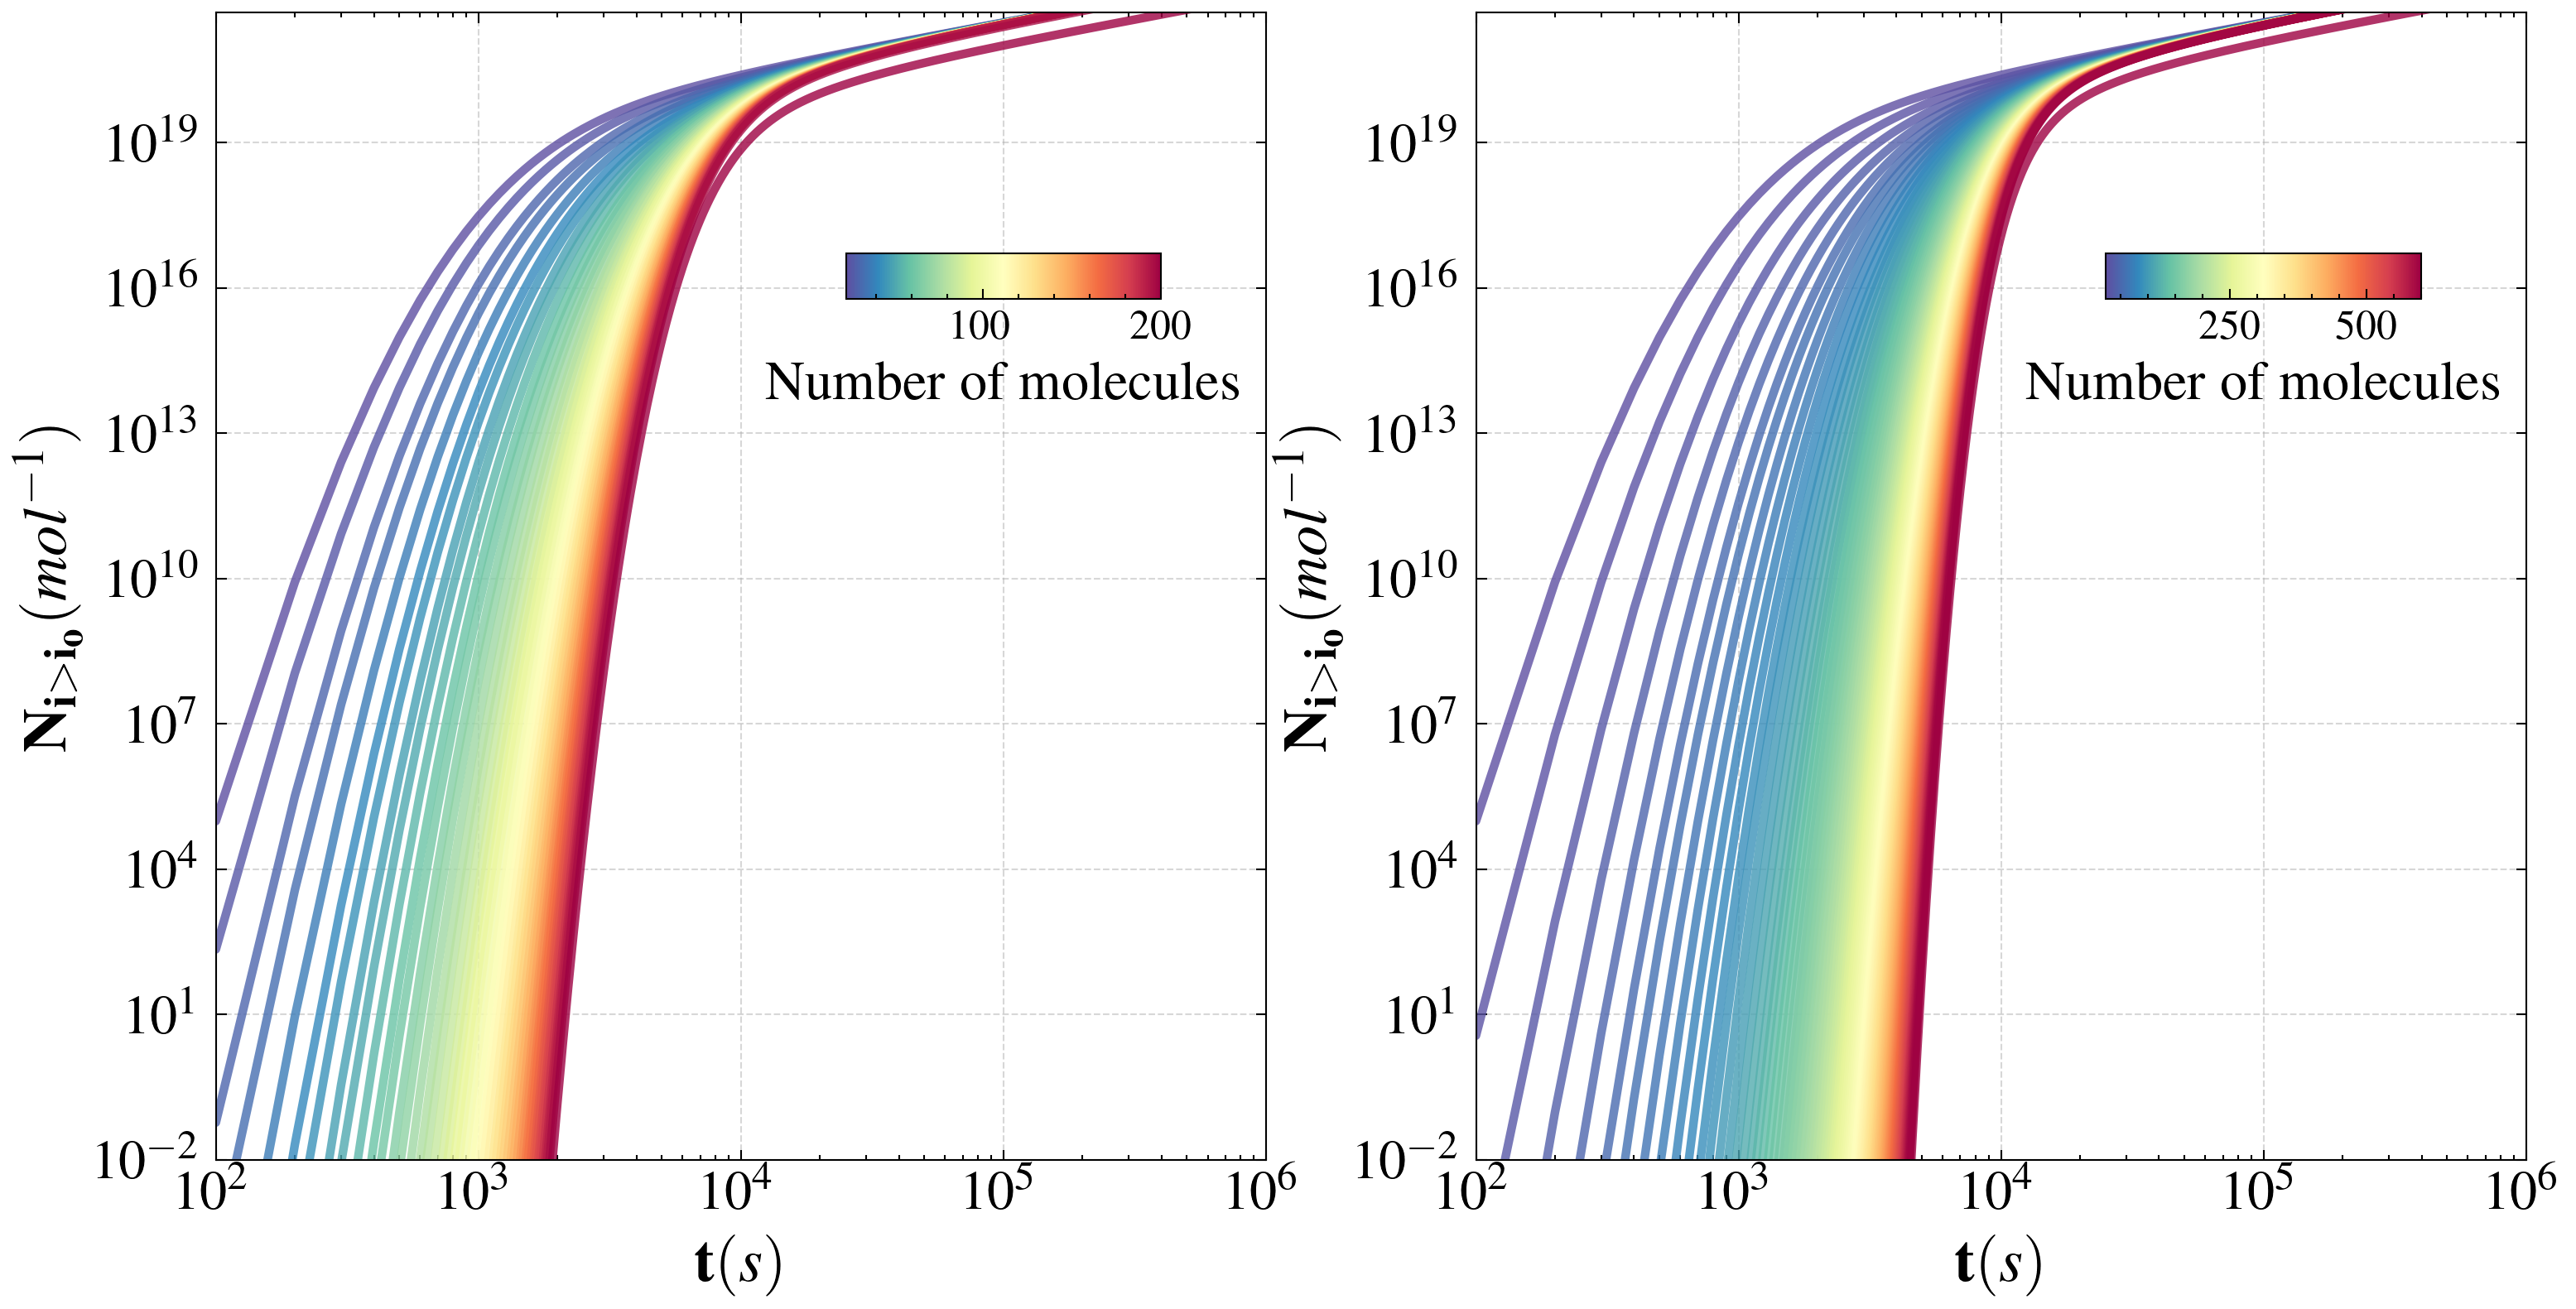
\includegraphics[width=1.1\linewidth]{postcritical_number_density_cr_particles_comparison.png}
    \caption{Iron postcritical total number density for different observable sizes for $i_{\text{max}} = 200$ (left) and $600$ (right).}
    \label{fig:postcritical_number_density_fe_particles_comparison}
\end{figure}

\paragraph{AlN}~\\
\vspace{1mm} % Adjust the space as needed

In this case, for the impurity Al-N, no phase diagram with lithium has been found, ideally a ternary diagram would be available in great detail, but the biography is very scarce, only a 
ternary diagram has been found but with little detail.\cite{Zhu}
The only phase diagram with minimal detail available is that of the Li-Al system from FactSage. While it is not accurate to directly assume 
that the Li-Al-N system will exhibit identical behavior, for the sake of analysis, we might consider similarities. According to the phase diagram, at the 
operating temperature specific to lithium, a significantly high fraction of aluminum (Al) is necessary for the formation of two distinct phases. In the absence 
of sufficient aluminum, the system is expected to remain entirely in the liquid state.

\begin{figure}[H]
    \centering
    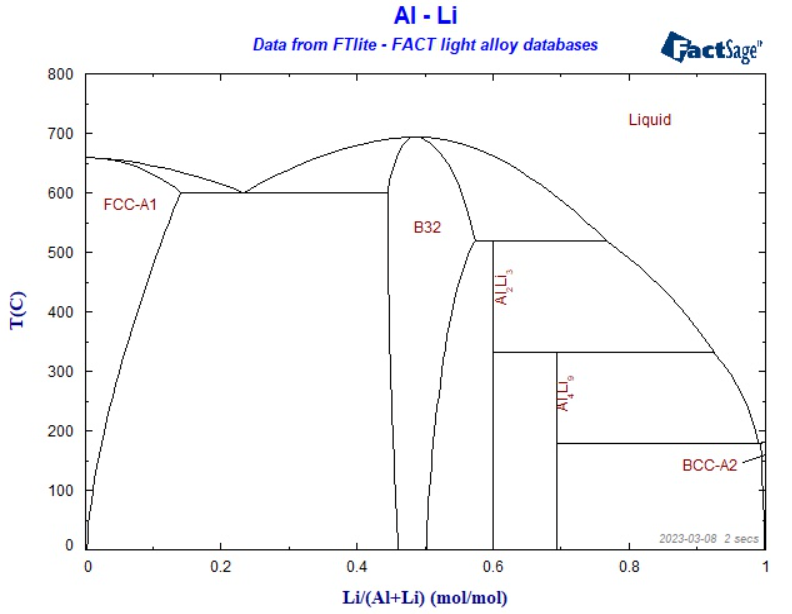
\includegraphics[width=0.9\linewidth]{al_li_diagram.png}
    \caption{Temperature dependence of hydrogen isotope solubility in lithium. \cite{Bale2016}.}
    \label{fig:al_li_diagram}
\end{figure}


Additionally, information on the diffusivity of Al-N in lithium is lacking. The only rigorous reference identified pertains to the diffusivity of different phases of Al-N \cite{CROWLEY2022231973}.
Due to the uncertainty surrounding the variables, it would be premature to present results that may not accurately reflect reality. Therefore, we propose deferring a more detailed investigation of this 
impurity to secure more reliable thermodynamic and kinetic parameters. Consequently, this deliverable will exclude simulations involving this specific impurity.

\subsubsection{Non-metallic impurities}
\paragraph{LiH, LiD, LiT}~\\
\vspace{1mm} % Adjust the space as needed

The system consisting of lithium, lithium hydride, and hydrogen (Li-LiH-H2) has undergone numerous studies. References where solubilities are experimentally found have been reviewed \cite{Veleckis1974THELH,Smith1979,Wang2012,Katsuta1977,Veleckis1977}. 
In \cite{Smith1979}, experimental isotherms were obtained, 
Values have been compared with each other and the values are consistent. 
Each of the isotherms is comprised of three regions. The first rising portion represents hydrogen reacting with and dissolving in lithium to produce a homogeneous 
liquid phase of lithium hydride dissolved in lithium. The constant pressure plateau defines the two-phase coexistence region. The boundaries of the plateau give the 
composition of the two coexisting phases. One phase is rich in lithium and contains dissolved lithium hydride. The other phase is rich in lithium hydride and contains 
dissolved lithium. As a hydrogen isotope is added to the system in this region, the amount of the lithium-rich phase decreases, and the amount of the lithium hydride-rich 
phase increases, but the composition of each phase remains constant. Within experimental accuracy, the boundaries (miscibility gap) and, therefore, the composition of the 
two phases were identical for the Li-LiH-H$_2$ and Li-LiD-D$_2$ systems. The second rising portion represents the homogeneous phase of lithium dissolved in liquid lithium hydride.


The experimental data are considered in terms of the equilibrium:

\begin{equation}
\frac{1}{2} H_2(g) + Li_{(\text{soln})} \rightleftharpoons LiH_{(\text{soln})}
\end{equation}

where $H$ represents any of the hydrogen isotopes. The equilibrium constant for the above reaction is:

\begin{equation}
K = \frac{N_{LiH} \gamma_{LiH}}{N_{Li} \gamma_{Li} \sqrt{P_{H2}}}
\label{eq:equilibrium_constant_h}
\end{equation}

Within the concentration range, Eq. \ref{eq:equilibrium_constant_h} can be rearranged to give the Sieverts relationship:

\begin{equation}
\sqrt{P_{H_2}} = K_s N_{LiH}
\end{equation}

The solubilities chosen as design variables are shown below.
\begin{figure}[H]
    \centering
    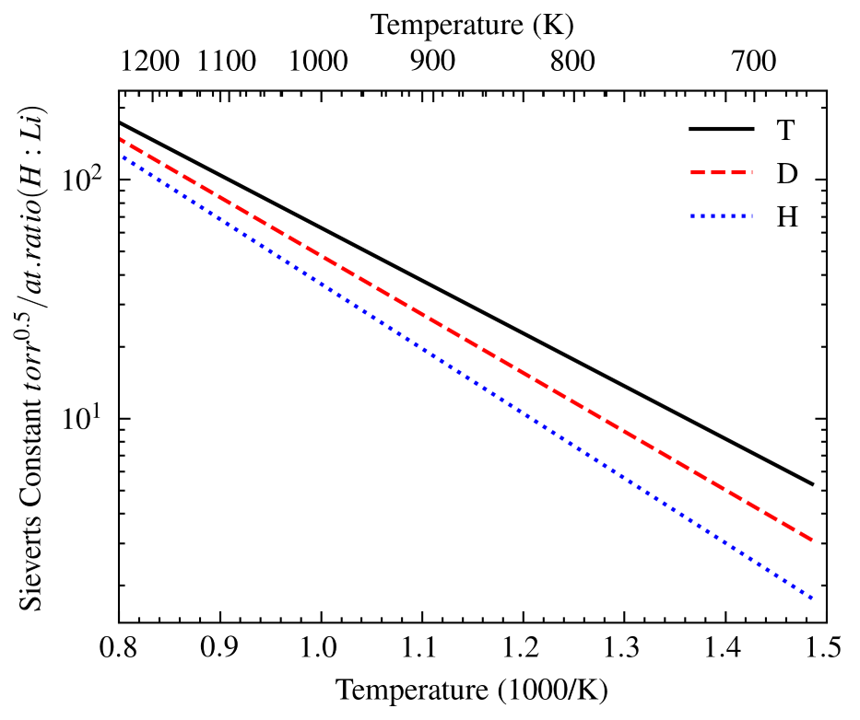
\includegraphics[width=0.8\linewidth]{hydrogen_solubility.png}
    \caption{Phase diagram of Li-Al mixture from FactSage database \cite{Bale2016}.}
    \label{fig:al_li_diagram}
\end{figure}

\newpage

\section{CENTRIFUGAL TECHNOLOGY SELECTION} \label{sec:eng}% ··························································
With the aim to review the available commercial centrifuges, the current section analyses its application for the purification loop of the RC. \\

\noindent The baseline for the given technologies in sections \ref{sec:sss} and \ref{sec:mss} is taken from the SoA report \cite{SoA}, where centrifuge devices for liquid-liquid and liquid-solid separators has been analyzed. 

\subsection{Single Step Separation Approach}\label{sec:sss}
The aim of this study is to provide the centrifuge technology/ies for FLF primary loop with the purpose to extract the solid impurities in the system. The captured requirements for the impurity loop of FLF has been identified as follows:

\begin{itemize}
	\item Continuous solid impurity extraction.
	\item Material compatibility.
	\item Energy efficiency.
	\item Efficiency for given particle size. 
	\item Operating temperature.
	\item Maintenance and cleaning.
	\item Scalability: maximum flow rate.
	\item Scalability: pressure drop.
	\item Concentration of impurities. 
	\item Residence time.
\end{itemize}

\begin{tcolorbox}[colback=gray!5!white,colframe=gray!75!black,title=Disclaimer]
	The requirements outlined herein pertain specifically to centrifuge technologies and serve as the foundational basis for the current project. Please note that these requirements are not exhaustive and may be subject to expansion or modification as the project progresses through subsequent stages. 
\end{tcolorbox}

\noindent The technologies can be compared based in the criteria given by the requirements, in order to capture which device or set of devices meet successfully the limited framework. Figure \ref{rad_chart} shows a radar chart with the aim to provide a benchmark based on 8 criteria aligned with the solid separator baseline.  

\begin{figure}[H]
	\centering
	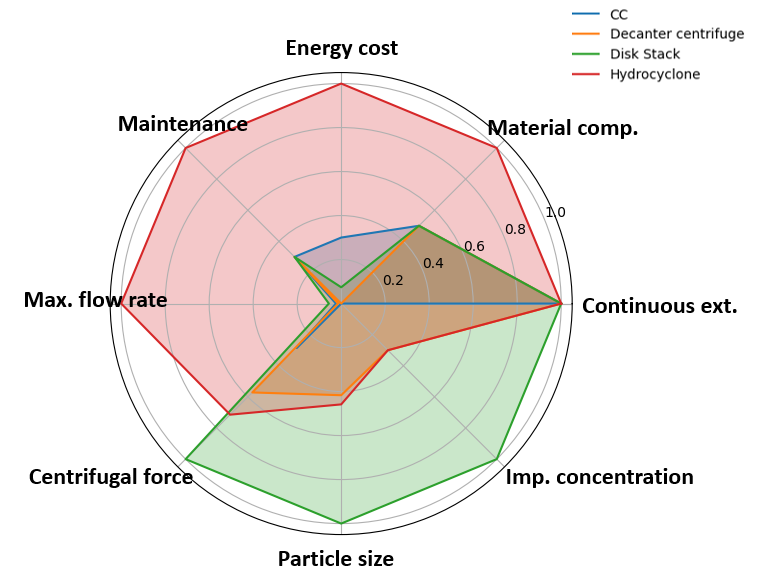
\includegraphics[width=0.85\linewidth]{rad_chart.png}
	\captionsetup{font=bf, size=small}
	\caption{Centrifugal technologies comparison chart}
	\label{rad_chart}
\end{figure}
\begin{figure}[H]
	\centering
	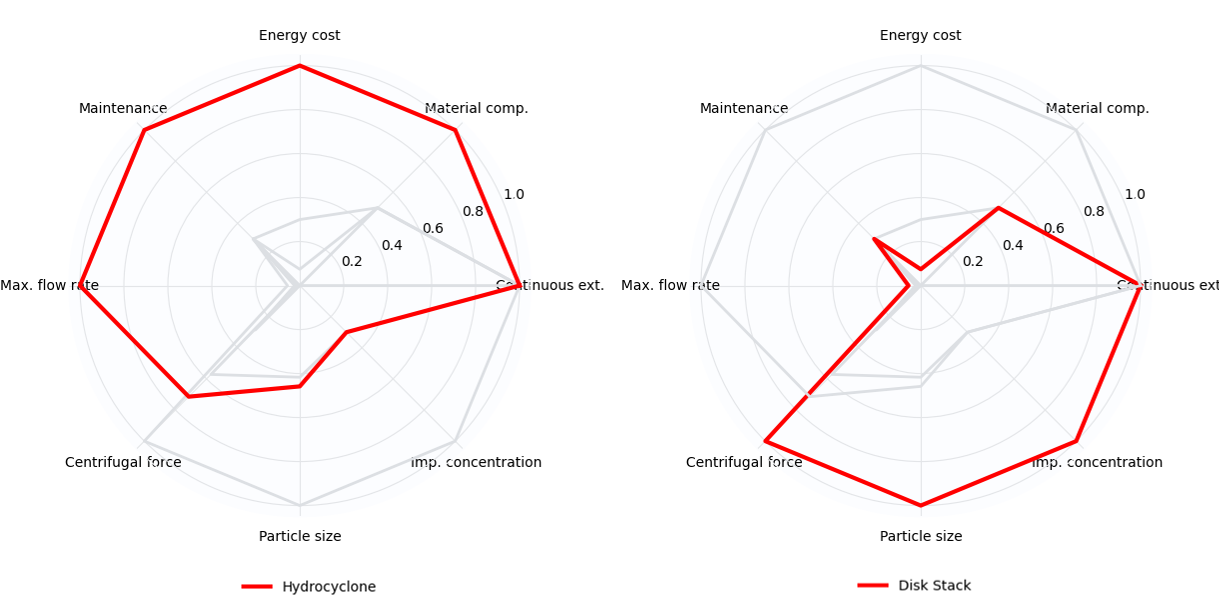
\includegraphics[width=1\linewidth]{rad_chart_comp.png}
	\captionsetup{font=bf, size=small}
	\caption{Hydrocyclone vs Disk Stack separator: radar plot results}
	\label{rad_chart_comp}
\end{figure}

\noindent Figure \ref{rad_chart} shows the performance of 4 centrifugal technologies, with a direct comparison for 8 scores (table \ref{rad_values} has the values used for the comparison, that has been normalized, and inverted for Energy Cost, Particle Size, Imp. Concentration). Hydrocyclone and Disk Stack Separator are the technologies with better performance in the evaluated fields, better single definition can be found in figure \ref{rad_chart_comp}, where:

 \begin{tcolorbox}[colback=blue!5!white,enhanced,breakable,colframe=blue!75!black,title=Hydrocyclone]
 	
 	\textbf{\textit{Advantages:}}
 	\begin{itemize}
 		\item Material compatibility: The hydrocyclone can be constructed using stainless steel, with SS16 being a commercially available option. Additionally, it can be fabricated from Fiber Reinforced Polymers (FRP), offering notable advantages in aggressive environments such as those found in chemical and nuclear applications with activating products. This versatility in material selection ensures adaptability to varying operational requirements and environmental conditions, enhancing the hydrocyclone's reliability and longevity in demanding settings.
 		\item Maintenance: Characterized by its absence of rotatory components, comprising four conical segments interconnected via flange bolted connections. This design feature ensures facilitated access to the internal cavity, enabling procedures for cleaning, replacement, or repair purposes.
 		\item Energy cost: The inherent design features, including a tangent inlet inducing a vortex through the cone, eliminates the necessity for moving parts, thus precluding the need for an engine. This architectural advantage translates into significant energy savings, as the hydrocyclone operates without any associated energy costs. Moreover, rigorous examination of inlet velocity's impact underscores the meticulous engineering approach applied to optimize performance.
 		\item Flow rate: It demonstrates superior flow rate management in comparison to the other three analyzed technologies. Moreover, it is commercially available to operate within a manifold architecture, allowing for efficient handling of large volumes. Consequently, it emerges as a prime candidate for processing the primary loop lithium in a single operation.
 	\end{itemize}
 	
 	\textbf{\textit{Disadvantages:}}
 	
 	\begin{itemize}
 		\item Particle size: Commercially available up to a particle size of 12 $\mu m$, with an impressive efficiency rate of 98\%, while maintaining scalability with a compromise on pressure drop (10-200 KPa). This equilibrium represents the optimal trade-off. Consequently, particles below 12 $\mu m$ can be captured by the hydrocyclone; however, ensuring consistent efficiency for particles of this size is not assured. Therefore, additional stages specifically designed for particles of this size range must be incorporated into the purification system to ensure thorough filtration and purification.
 		\item Impurity concentration: The technology's optimal operational range encompasses concentrations of impurities in the medium exceeding 10\%. Therefore, it is recommended to position this technology as the initial stage within the purification system. This strategic placement ensures efficient removal of contaminants at higher concentrations, thereby enhancing the overall effectiveness of the purification process. Future stages may address more accurate the impurity concentration in the system.
 	\end{itemize}
 	
 	\textbf{\textit{Assessment:}} The hydrocyclone offers exceptional material compatibility, maintenance-friendly design (without of rotatory components), with negligible energy costs and superior flow rate management, based on manifold architectures: the hydrocyclone emerges as an ideal candidate for processing the primary loop fluid. Despite limitations in capturing particles below 12 $\mu m$ and optimal operation at impurity concentrations exceeding 10\%, strategic integration within purification systems enhances overall effectiveness.
 	
 \end{tcolorbox}
 \begin{tcolorbox}[colback=blue!5!white,enhanced,breakable,colframe=blue!75!black,title=Disck Stack Separator]
		\textbf{\textit{Advantages:}}
	\begin{itemize}
		\item Particle size: One of the most notable strengths of this technology lies in its ability to effectively capture particles as small as 1 $\mu m$, facilitated by its high centrifugal force and innovative ribs cavity design, which accelerates solid precipitation. Particularly advantageous in scenarios where prior classification or clearance of larger particle sizes has been performed, allowing for optimal exploitation of its particle-capturing capabilities.
		\item Impurity concentration: The operational range for these devices remains optimal when impurity concentrations are below 10\%, presenting an advantageous characteristic when integrated into multi-stage system operations.
		\item Centrifugal force: As a high-speed separator capable of achieving up to 14,000 G, the disk stack separator offers a distinct advantage due to its efficient operation at relatively low energy costs, contrasting with decanter centrifuges. While centrifuge contractor may require similar energy inputs, they do not attain comparable levels of centrifugal force, highlighting the disk stack separator's pivotal role in separation processes based on its design principles.
	\end{itemize}
	
	\textbf{\textit{Disadvantages:}}
	
	\begin{itemize}
		\item Energy cost: Exhibits relatively higher energy consumption compared to alternative solutions. This aspect should be considered in the evaluation of operational costs and efficiency metrics within the full-scale context.
		\item Maintenance: The trade-off associated with attaining high-speed rotation velocities may influence the maintenance of components, wherein direct access to elements is not a direct action, requiring mechanical assembly-disassembly processes that are less straightforward compared to hydrocyclones.
		\item Flow rate: The limited maximum flow rate capacity of such devices makes them unsuitable for fully processing all the lithium within the primary loop. Furthermore, the absence of commercially available manifolds presents a challenge. Therefore, a rigorous study could be needed to strategically place these devices within the system, coupled with the feasibility assessment for developing a manifold configuration to optimize operational efficiency.
	\end{itemize}
	
	\textbf{\textit{Assessment:}} The Disk Stack Separator offers good particle capture capabilities, particularly for particles as small as 1 $\mu m$, making it ideal for scenarios requiring precise filtration after prior particle classification. However, its higher energy consumption and maintenance complexities warrant careful consideration. When compared with hydrocyclones, which excel in energy efficiency and maintenance simplicity, they form complementary components in a comprehensive purification system, each tailored to specific operational requirements and constraints. Integrating both technologies strategically within a multi-stage system can optimize overall efficiency and performance, complementing their disadvantages.
	
	
\end{tcolorbox}
 \begin{tcolorbox}[colback=blue!5!white,enhanced,breakable,colframe=blue!75!black,title=Decanter Centrifuge]
	Decanter centrifuges demonstrate comparable performance to hydrocyclones in particle size handling, centrifugal force generation, and impurity concentration control. However, hydrocyclones offer superior energy efficiency, enhanced material compatibility, and lower maintenance requirements, presenting clear advantages. Notably, hydrocyclones excel in maximizing the maximum flow rate, making them a preferred choice in scenarios prioritizing throughput efficiency and operational cost-effectiveness.
\end{tcolorbox}
 \begin{tcolorbox}[colback=blue!5!white,colframe=blue!75!black,title=Centrifuge Contactor]
	While centrifuge contactors offer the advantage of producing four-phase liquid separation, they do not present a significant advantage in the fields compared to hydrocyclones. The technology lacks suitability in efficiently handling impurities at required flow rates with the precision demonstrated by alternative technologies, diminishing its practical utility in for the primary loop.
\end{tcolorbox}

\newpage
\subsection{Multi-Step Separation Approach}\label{sec:mss}
In the context of a multi-stage separation process, the integration of hydrocyclones and Disk Stack Separators offers a comprehensive solution for fluid purification. The hydrocyclone, as particle cut-off controlled by operation parameters, is particularly adept at classifying and separating coarser particles ($>$ 12 $\mu m$), thereby facilitating the initial removal of larger impurities. Its attributes, including superior material compatibility and a maintenance-friendly design, make it a suitable choice for efficiently processing substantial fluid volumes, thanks to its ability to handle high flow rates and adapt to various manifold configurations.\\


\noindent However, the hydrocyclone's inherent limitations, such as its inability to capture particles below 12 $\mu m$ and its optimal operation in scenarios with impurity concentrations above 10\%, necessitate additional stages for thorough purification. This is where the Disk Stack Separator comes into play, especially in scenarios where specific targets, such as low impurities or activated products separated by density differences like Li-H, need to be addressed. Renowned for its exceptional particle capture efficacy, particularly for particles as small as 1 $\mu m$, the Disk Stack Separator strategically placed downstream of the hydrocyclone enhances the purification process by effectively removing finer particles and residual impurities at low concentrations (up to 0.05\%), thereby ensuring the level of lithium purity.\\


\noindent Despite its advantages, the Disk Stack Separator incurs relatively higher energy consumption and maintenance complexities compared to the hydrocyclone. Therefore, meticulous attention is needed in optimizing the integration of these technologies to ensure overall efficiency. For example, incorporating the Disk Stack Separator as a secondary stage in the purification process allows for precise filtration after larger particles have been removed by the hydrocyclone, as shown in Figure \ref{multi_stage}. At the same time, it raises the requirement to project a future device that captures the high efficiency for small particles at the energy cost and lithium volumes of the hydrcyclone.

\begin{figure}[H]
	\centering
	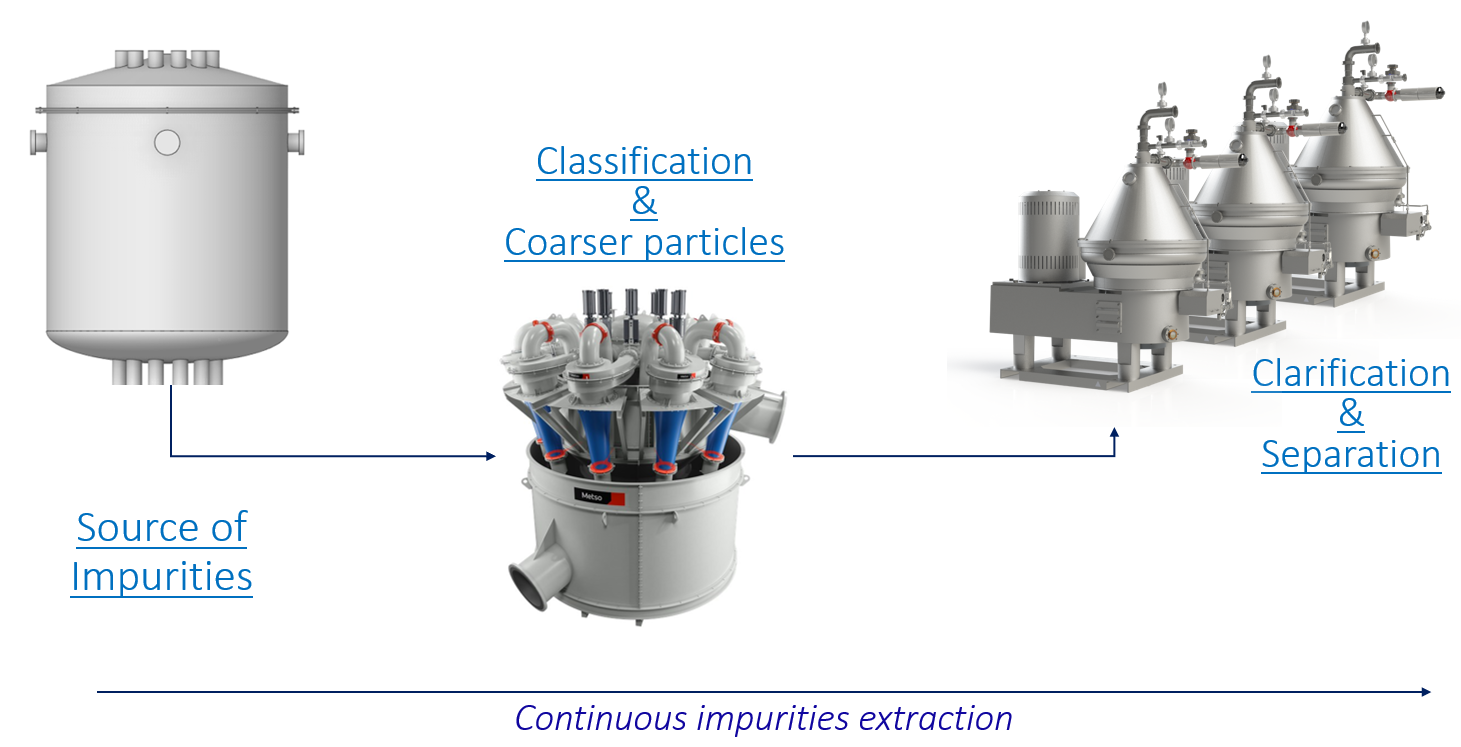
\includegraphics[width=0.9\linewidth]{multi_stage.png}
	\captionsetup{font=bf, size=small}
	\caption{Multi stage configuration}
	\label{multi_stage}
\end{figure}

\noindent In this multi-stage paradigm, the symbiotic relationship between the hydrocyclone and Disk Stack Separator maximizes each technology's strengths while mitigating respective weaknesses. \\

\noindent The relevant technical specifications for both technologies are delineated in Figure \ref{multi_stage_technical}. This technical data serves as the foundational benchmark for subsequent stages of the project, guiding the development of solutions aligned with the current multi-stage framework. The analysis of this data informs decisions regarding the integration of technologies, aiming to optimize the process schema and ultimately enhance overall efficiency and effectiveness.

\begin{figure}[H]
	\centering
	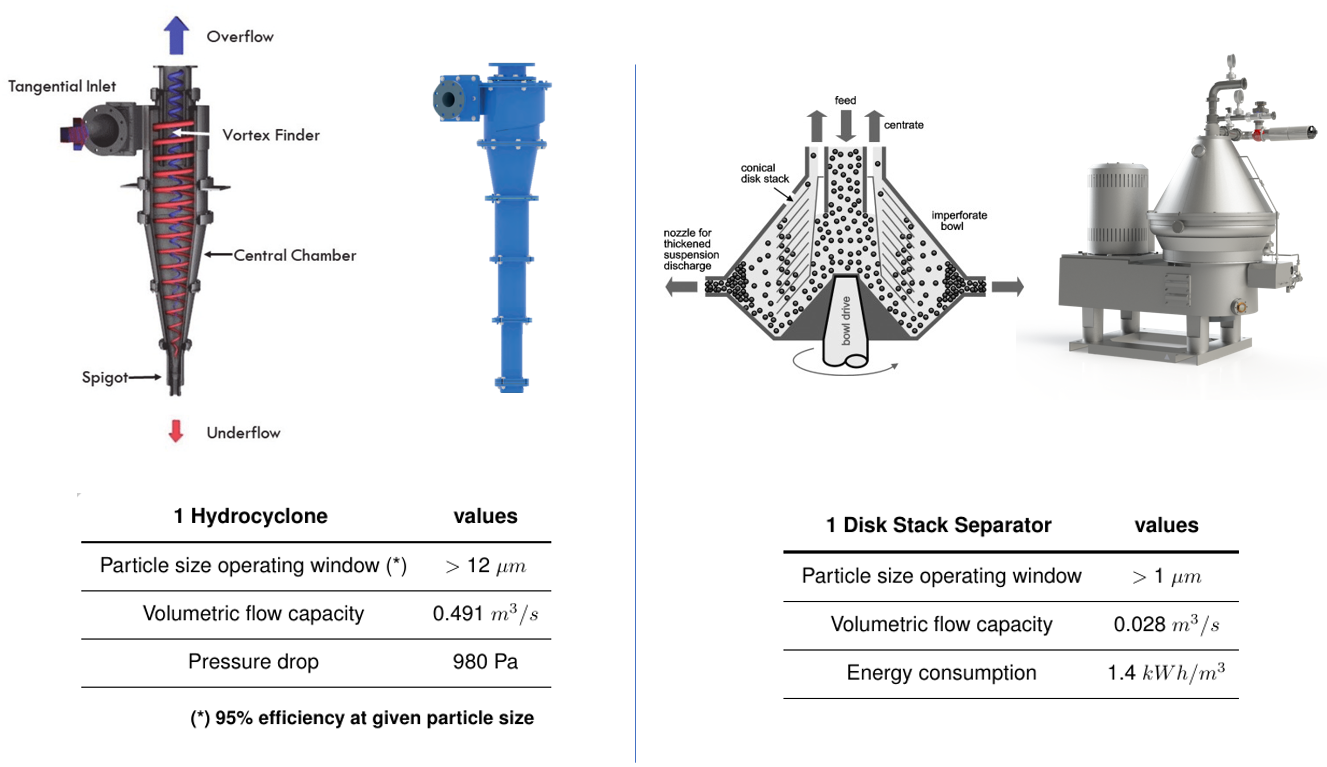
\includegraphics[width=1\linewidth]{multi_stage_technical.png}
	\captionsetup{font=bf, size=small}
	\caption{Multi stage device data-sheet}
	\label{multi_stage_technical}
\end{figure}

\newpage
\subsection{Hydrocyclone: Mathematical modelling}

%\section{Mathematical model}
Cyclone separators are widely used in the field of chemical, mine and petroleum industries. ref.\cite{Concha2007} With the advantages of relative simplicity to fabricate, low cost to operate and good adaptability to extremely harsh conditions, cyclone separators have become one of the most important particle removal devices which are preferably utilized in both environmental and chemical engineering.
In order to describe the performance of cyclone separators, many (gas or liquid)-particle separation theories were developed using different methods with different simplifications and assumptions.
All these can be roughly divided into the pure theory, the semi-empirical theory and the numerical simulation. The former two include the equilibrium-orbit model, time-of-flight model and hybrid model, etc., the later mainly refers to the computation fluid dynamics (CFD) approach ref.\cite{Altmeyer2003}.

In detail, the equilibrium-orbit model, as an early methodology of particle separation, determines the particle size for which centrifugal force is exactly balanced by the drag force. Correspondingly, the collection efficiency for the critically sized particle is often assumed to be 50\% efficiency called cut particle diameter $d_{c,p}$ ref.\cite{Zhao2011}.

 In this section, the necessary parameters and assumptions are defined to correctly define the equilibrium orbit model and obtain an expression for the cyclone separation efficiency.
 \begin{tcolorbox}[colback=blue!5!white,colframe=blue!75!black,title=Assumptions]
The following assumption have been made in order to develop the equilibrium-orbit model ref. \cite{Wei2016}: 
\begin{itemize}
	\item The particle is spherical in shape, the motion of the single particle is not influenced by the presence of neigh-boring particle.
	\item The tangential velocity of the particle is same as the disperse phase stream; and with the particle is the right dispersed phase, the radial velocity direction fo the particle always point to inner vortex.
	\item  The particle move into the inner vortex is the only way to be separated.  
\end{itemize}
\end{tcolorbox}


Figure (\ref{cyclone_schema}) show a generic scheme of the cyclone and the description of the different variables is presented in table (\ref{variable_cyclone_description}).


\begin{figure}[H]
	\begin{minipage}[b]{.4\linewidth}
		\centering
		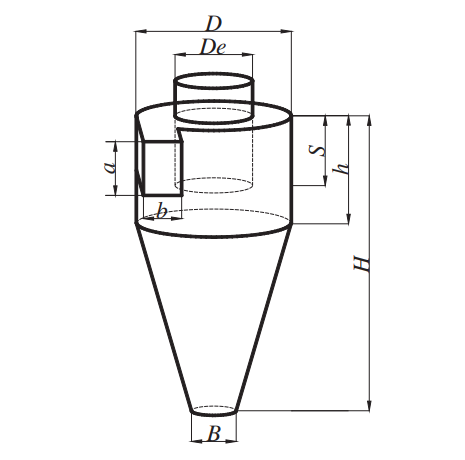
\includegraphics[width=1\linewidth]{images/schema.png}
		\captionsetup{font=bf, size=small}	
		\captionof{figure}{Schematic diagram of typical cyclone dimensions.}
		\label{cyclone_schema}
	\end{minipage}\hfill
	\begin{minipage}[b]{.59\linewidth}
		\centering
	\begin{tabular}{cc}
		\hline
			\rule[-0.3cm]{0pt}{0.8cm}\textbf{variable} & \textbf{description}                                \\ \hline
			\rule[-0.3cm]{0pt}{0.8cm}$a$                 & Cyclone inlet height (m)                            \\ \hline
			\rule[-0.3cm]{0pt}{0.8cm}$b$                 & Cyclone inlet width (m)                             \\ \hline
			\rule[-0.3cm]{0pt}{0.8cm}$B$                 & Particle outlet diameter (m)                        \\ \hline
			\rule[-0.3cm]{0pt}{0.8cm}$D$                 & Cyclone body diameter (m)                           \\ \hline
			\rule[-0.3cm]{0pt}{0.8cm}$D_e$              & Liquid outlet diameter (vortex finder diameter) (m) \\ \hline
			\rule[-0.3cm]{0pt}{0.8cm}$h$                 & Cyclone cylinder height (m)                         \\ \hline
			\rule[-0.3cm]{0pt}{0.8cm}$H$                 & Cyclone height (m)                                  \\ \hline
			\rule[-0.3cm]{0pt}{0.8cm}$S$                 & Liquid outlet duct length (m)                       \\ \hline
	\end{tabular}
		\captionof{table}{Description of the geometrical variables of one cyclone.}
		\label{variable_cyclone_description}
	\end{minipage}
\end{figure}


\subsection{Fluid model}
%For this problem there are 2 types of phenomena present to describe the flow pattern. The first zone is called the forced vortex, which occurs between r=0 and r=b/2 approximately where the tangential velocity is linear with the angular velocity w (v=w r). On the other hand, we have a free vortex given by the equation:

Swirling flow, or vortex flow, occurs in different types of equipment, such as cyclones, hydrocyclones, spray dryers and vortex burners. Two types of ideal swirling flows are ref.\cite{Marthinussen2011}: 
\begin{itemize}
	\item Forced vortex flow: swirling flow with the same tangential velocity distribution as a rotating solid body.
	\begin{equation}
		v_{\theta,f}=\omega r 
	\end{equation}
	\item Free vortex flow: the way a frictionless fluid would swirl. The tangential velocity in such a swirl is such that the moment-of-momentum of fluid elements is the same at all radius. 
	\begin{equation} \label{free_vortex_flow}
		v_{\theta,f}(r)=\frac{\kappa}{r^n} \text{  where } 0.4<n<0.9 
	\end{equation}	
	where $\kappa$ is a geometrical parameter and $n$ is a experimental value taken 0.88 as in ref.\cite{Sabbagh2014} 
\end{itemize} 
Figure (\ref{tangential_velocity}) show the schema of the real tangential velocity distribution and the comparison with the forced and free vortex flow.

\begin{figure}[H]
	\centering
	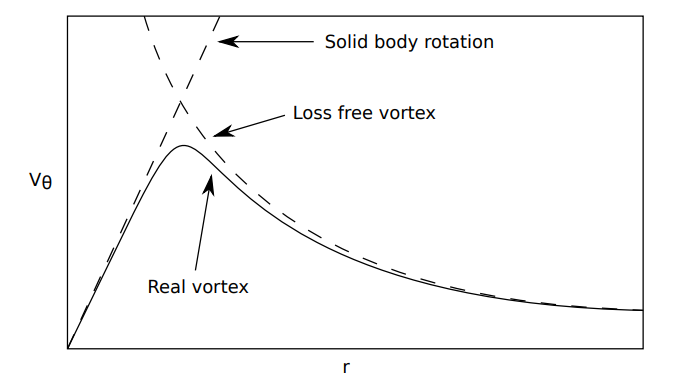
\includegraphics[width=0.5\linewidth]{images/tangential_velocity_schema.png}
	\captionsetup{font=bf, size=small}
	\caption{Scheme of the 2 ideal vortex model and the tangential velocity distribution in a real vortex. ref.\cite{Marthinussen2011}}
	\label{tangential_velocity}
\end{figure}

\subsection{Motion of suspended particles}
In a hydrocyclone, the particles of interest are almost always moving relative to the liquid at their terminal velocity, and the terminal velocity of a given particle determines whether the particle will be captured or lost.

Applying Newton’s law to a particle moving in a fluid, equating its mass times acceleration to the sum of the forces acting on it, gives :
\begin{equation}
	m \frac{d v}{d t}= F_{body} + F_{drag} + F_{unsteady}
\end{equation}
where the body force is normally due to a centrifugal force and the fluid drag represents the drag acting on a
particle that moves with a steady velocity relative to the fluid ref.\cite{Sabbagh2014} .
According to several authors ref.\cite{Concha2007,Marthinussen2011}, it turns out that these unsteady terms can be ignored both for the case of a gas cyclone and a hydrocyclone, as practical plant experience with their design and operation indicates that it is not necessary to include either of the terms.


%\subsubsection*{Centrifugal Force}
The centrifugal force (first term on the right part ) can be expressed as :
\begin{align}
	F_{body}=F_{centrifugal}=V_p \left( \rho_p-\rho_{f} \right) \textbf{a}
\end{align}
where $V_p$ is the particle volume, $\rho_p$ is the particle density, $\rho_f$ is the fluid density and $\textbf{a}$ is the global effect of the radial and angular particle acceleration. 

In cylindrical coordinate, omitting the axial contribution, 
\begin{itemize}
	\item $a_r= \frac{d v_{r,p}}{d t}= \frac{d^2 r}{d t^2 }$ particle radial acceleration 
	
	\item $a_c= r \left( \frac{d \theta}{d t}\right)^2= r \left(\frac{v_{\theta,f} (r)}{r} \right)^2 $ particle angular acceleration
	
\end{itemize}
assuming that the radial particle acceleration in the steady state is negligible, the centrifugal force is equal to:
\begin{equation}
	F_{centrifugal}= \frac{1}{6} \pi d_p ^3 \cdot (\rho_p -\rho_f) \cdot \frac{v_{\theta,f} ^2(r)}{r}
\end{equation}

%\subsubsection*{Drag Force}
on the other hand, when the particle Reynolds number is low ($Re_p = \frac{d_p v_{r,p}}{\nu}<<1$), the
equations of motion for the fluid moving around the particle can be solved, and the drag force 
calculated. If there is no slip between fluid and particle surface, the particle velocity is
equal to the velocity of the fluid at the surface, the result is Stokes drag law: 
\begin{equation}
	F_{drag}=3 \pi  \mu d_p v_{r,p}(r) 
\end{equation}
Therefore, in the steady state, the drag force have to be equal that the centrifugal force:

\begin{equation}
	\sum F_p = 0 \Rightarrow F_{centrifugal}= F_{drag}  
\end{equation}
and the radial velocity of the particle can be expressed as a function of the angular velocity of the fluid given by the vortex flow model as
\begin{equation} \label{radial_velocity_particle}
	v_{r,p}(r)= \frac{\Delta \rho d_p ^2   }{18 \mu } \cdot \frac{v_{\theta,f}^2(r)}{r}
\end{equation}


The following subsections define different parameters necessary to calculate the cyclone separation efficiency.


\subsection{Cyclone effective volume}
To avoid the non-uniform effect on particle collection distance caused by difference between cylindrical and conical shape, the cylinder-conical geometry is equivalently modified as a right cylinder cyclone according to the principle of conservation of effective volume.
The equivalent cyclone volume ($V_{cs}$) and  radius ($R$) can be calculated by: ref.\cite{Zhao2011}
\begin{equation}
	V_{cs}=
	\begin{cases}
		 \frac{\pi D^2 h}{4} +\frac{\pi D^2 }{4} \cdot \frac{S+l-h}{3} \cdot \left[ 1+ \frac{D_c}{D}+ \left(\frac{D_c}{D} \right)^2  \right] ,& \text{if } l\leq (H-S)\\
		\frac{\pi D^2 h}{4} +\frac{\pi D^2 }{4} \cdot \frac{H-h}{3} \cdot \left[ 1+ \frac{B}{D}+ \left(\frac{B}{D} \right)^2  \right],& \text{if } l> (H-S)
	\end{cases}
\end{equation}



\begin{equation} \label{effective_radious_equation}
	{R^*} _w= 
	\begin{cases}
		\left[ \frac{V_{cs}}{\pi (S+l)}\right]^{1/2} ,& \text{if } l\leq (H-S)\\
		\left[ \frac{V_{cs}}{\pi H}\right]^{1/2},& \text{if } l> (H-S)
	\end{cases}
\end{equation}
where $D_c= D - \frac{(D-B)(S+l-h)}{H-h}$ and $l$ is called as the natural vortex length of cyclone separator. It is defined as the vertical distance from the bottom of the vortex finder to the end of the vortex at which the outer vortex is reversed or turned into the inner vortex. $l$ is actually the effective vortex length in cyclone separator if it is less than the dimension $H–S$. Otherwise, $H–S$ should be the effective vortex length because it depends on the geometrical dimensions of cyclone.
The most famous and widely used relation for estimating the natural vortex length is the Alexander’ formula ref.\cite{Zhao2011}: 
\begin{equation}
	l=2.3 \left( \frac{D^2}{a b}\right)^{1/3}
\end{equation}

\subsection{Residence time model} 
The residence time $t_{res}$ is the average time  that a particle is inside the cyclone. The expression to calculate $t_{res}$ depend of the geometry of the cyclone and the inlet volumetric flow rate, so according to the geometry selected (Figure \ref{cyclone_schema}) the residence time can be calculates as ref.\cite{Zhao2011}:
\begin{equation}\label{residence_time_equation}
	t_{res}= 
	\begin{cases}
		\frac{\pi \left( R^2 - R_e ^ 2\right) }{Q/2} \cdot l,& \text{if } l\leq (H-S)\\
		\frac{\pi \left( R^2 - R_e ^ 2\right)}{Q/2} \cdot (H-S),& \text{if } l> (H-S)
	\end{cases}
\end{equation}

\subsection{Separation efficiency model}
In order to calculate the separation efficiency of the cyclone, a balance of mass was made in the volume of control presented in the Figure (\ref{volume_control}) ref.\cite{Zhao2011,Wei2016}.
\begin{figure}[H]
	\centering
	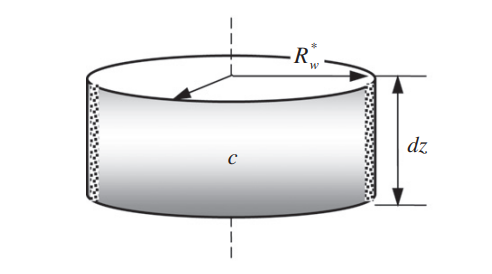
\includegraphics[width=0.5\linewidth]{images/control_volume.png}
	\captionsetup{font=bf, size=small}
	\caption{volume of control used in the separation efficiency model. ref.\cite{Zhao2011}}
	\label{volume_control}
\end{figure}
In this control volume, it is assumed that uncollected particles in any plane perpendicular to the cyclone axis presents a status of complete radial back-mixing, the boundary layer near the equivalent wall is neglected and particles which move to the equivalent wall will be trapped. If the particle concentration in the control volume is
$c$, then the particle flux toward the equivalent wall is $c v_{r,p}({{R^*}} _w)$ . Therefore, over a height $dz$ the sedimentation rate of particles at the equivalent wall is $ 2 \pi {{R^*}} _w c v_{r,p}({R^*} _w) $ . Correspondingly, the rate of particles separated from the control volume is $c \pi {{R^*}} _w^2 dz$.
According to particle mass balance, we have:


\begin{align}
	\frac{d M}{d t }=& \sum M_{in} -\sum M_{out}\\
	\frac{d(c \pi {R^*} _w^2 dz)}{dt}=& -\sum M_{out}= - c v_{r,p}({R^*} _w) 2 \pi {R^*} _w dz\\
	\frac{d c}{d t}=& - \frac{2v_{r,p}(R* _w)}{{R^*} _w} \cdot c \\
	\frac{c(t)}{c_0}=& exp \left(- \frac{2v_{r,p}({R^*} _w) t}{{R^*} _w} \right)
\end{align}

Integrating, with $c(t=0)=c_0$ and $c_{final}=c(t_{res})$ where $t_{res}$ is the particle residence time:

\begin{equation}
	\frac{c_{final}}{c_{0}}= exp \left(- \frac{2v_{r,p}({R^*} _w) t_{res}}{{R^*} _w} \right)
\end{equation}
therefore, the separation efficiency is defined as 
\begin{align} 
	\eta=&1-\frac{c_{final}}{c_{0}}\\
	\eta=&1- exp \left(- \frac{2v_{r,p}({R^*} _w) t_{res}}{{R^*} _w} \right) \label{efficiency_equation}
\end{align}
where $v_{r,p}({R^*} _w)$ is the particle settling velocity at the equivalent wall
and is calculated according to Eq. (\ref{radial_velocity_particle}) 

\section{Results: Parametric analysis}

For the following analysis, the geometric dimensions present in the table \ref{input_information} have been used as a basis. This information was used to see how the separation efficiency of the cyclone varies when the Lithium temperature, the diameter of the cyclone and the inlet flow change. 

\begin{table}[H]
	\centering
	\begin{tabular}{cc}
			\rule[-0.3cm]{0pt}{0.8cm} \textbf{variable} & \textbf{value} \\ \hline
			\rule[-0.3cm]{0pt}{0.8cm}\textbf{$D$}                            & 0.5 m          \\ \hline
			\rule[-0.3cm]{0pt}{0.8cm}\textbf{$\frac{De}{D}$}                        & 0.5            \\ \hline
			\rule[-0.3cm]{0pt}{0.8cm}\textbf{$\frac{a}{D}$}                         & 0.5            \\ \hline
			\rule[-0.3cm]{0pt}{0.8cm}\textbf{$\frac{b}{D}$}                         & 0.2            \\ \hline
			\rule[-0.3cm]{0pt}{0.8cm}\textbf{$\frac{S}{D}$}                         & 0.5            \\ \hline
			\rule[-0.3cm]{0pt}{0.8cm}\textbf{$\frac{H}{D}$}                         & 4              \\ \hline
			\rule[-0.3cm]{0pt}{0.8cm}\textbf{$\frac{h}{D}$}                         & 1.5            \\ \hline
			\rule[-0.3cm]{0pt}{0.8cm}\textbf{$\frac{B}{D}$}                         & 0.375          \\ \hline
			\rule[-0.3cm]{0pt}{0.8cm}\textbf{Fluid material}               & Lithium        \\ \hline
			\rule[-0.3cm]{0pt}{0.8cm}\textbf{Fluid Temperature}            & 688 K          \\ \hline
			\rule[-0.3cm]{0pt}{0.8cm}\textbf{Particle material}            & Fe            \\ \hline
	\end{tabular}
	\caption{Input information used for the parametric analysis section}
	\label{input_information}
\end{table}
\subsection{Parametric analysis: Temperature}
Figure (\ref{temperature_cyclone}) shows the efficiency as a function of the particle diameter of Fe for the temperature of the Start-Up, HEX outlet and lower tank calculated in ref. \cite{power_scenario}. 


\begin{figure}[H]
	\centering
	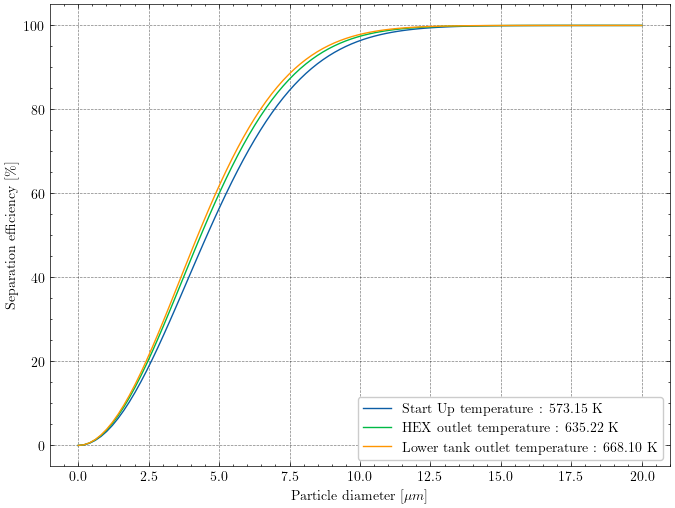
\includegraphics[width=0.5\linewidth]{images/efficiency_vs_Temperature.png}
	\captionsetup{font=bf, size=small}
	\caption{Separation efficiency as a function of the particle diameter of Fe for different temperatures.}
	\label{temperature_cyclone}
\end{figure}
As the temperature increases, the fluid viscosity decreases, so the drag force  decrease and the particle velocity increase. Also, the difference in density fluid-particle also increases (since the density of lithium decreases with temperature) so that the centrifugal force grow. Those effects allows efficiency to increase with temperature.
\subsection{Parametric analysis: Cyclone diameter}
Figure (\ref{cyclone_diameter})  shows the separation efficiency as a function of the particle diameter of Fe for different cyclone diameters.

\begin{figure}[H]
	\centering
	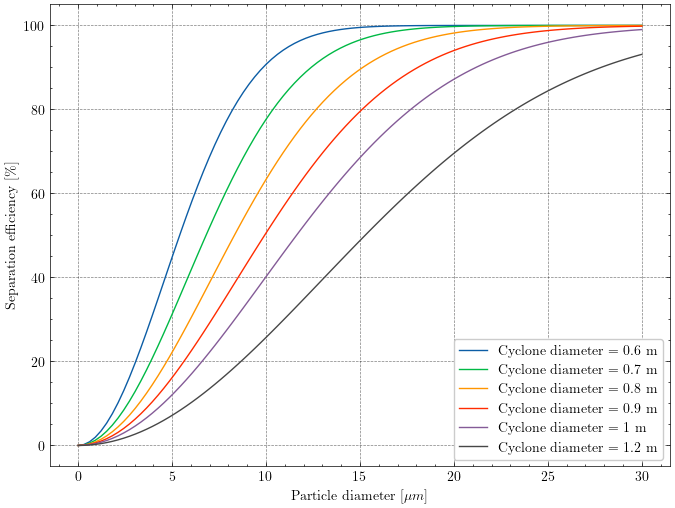
\includegraphics[width=0.5\linewidth]{images/efficiency_vs_cyclone_diameter.png}
	\captionsetup{font=bf, size=small}
	\caption{}
	\label{cyclone_diameter}
\end{figure}
By increasing the diameter and keeping the scaling and flow variables constant, the velocity in the inlet decreases. This decrease causes that the velocity of the particles to drop and the efficiency to drop. On the other hand, as the diameter increases, the residence time increases given by the equation (\ref{residence_time_equation}) and this effect tends to increase efficiency, however, it is not as important as the other effect mentioned before.

%By increasing the diameter,  it is possible to process more flow in each cyclone. However, the separation efficiency decreases. It is a compromise decision since is needed to know the minimum particle diameter that have to be eliminated.
Thus, there is a trade-off in deciding the optimal cyclone diameter, and it will also depend on the minimum particle diameter of the impurities which need to be eliminated.
\subsection{Parametric analysis: volumetric inlet flow rate}
Given one of the limitations of cyclones is the possibility of scaling efficiency to industrial-type flows, in the chemical or mine industry it is very common to use more than 1 cyclone in parallel ref. \cite{Concha2007}. For this reason it is of interest to know how the efficiency changes as we increase the volumetric inlet flow rate of the cyclone.

Figure (\ref{inlet_VRF}) show the separation efficiency as a function of the particle diameter for different volumetric inlet flow rate form from 0.5 to 3.5 $m^3/s$ (similar to pilot plant). 

\begin{figure}[H]
	\centering
	\begin{subfigure}{.49\textwidth}
		\centering
		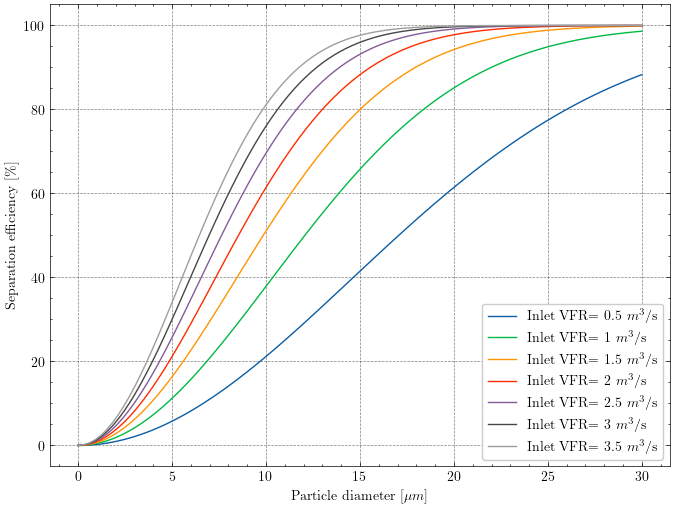
\includegraphics[width=1.0\linewidth]{images/efficiency_vs_inlet_VFR.png}
		\caption{}
		\label{inlet_VRF}
	\end{subfigure}
	\begin{subfigure}{.49\textwidth}
		\centering
		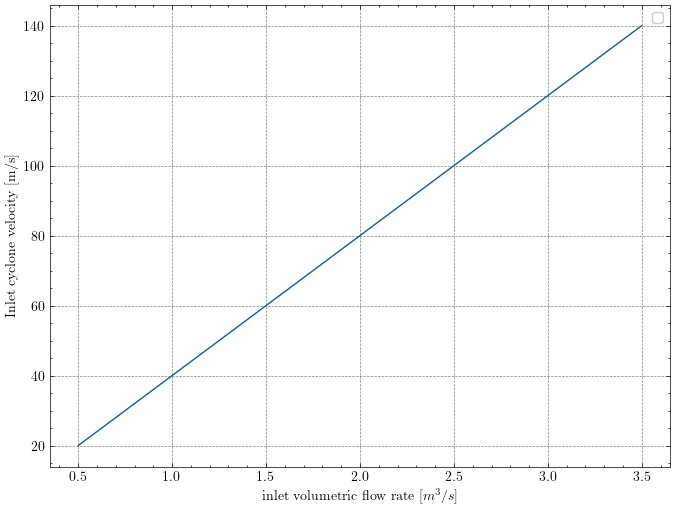
\includegraphics[width=1.0\linewidth]{images/inlet_VRF_vs_inlet_velocity.png}
		\caption{}
		\label{inlet_velocity}
	\end{subfigure}
	\captionsetup{font=bf, size=small}
	\caption{ }
	\label{}
\end{figure}

It can be seen that as volumetric flow rate decrease, the separation efficiency decreases. This is because as the flow rate at the inlet of the cyclone decreases, the velocity in the inlet drop (Figure \ref{inlet_velocity}) and consequently the velocity with which the particle heads towards the walls of the cyclone. It is important to note that industrial-scale cyclones usually operate with an inlet speed between 20-30 m/s, so this limitation should be added in the following sections to have a realist results.

Figure (\ref{inlet_VRF_porcent}) show the separation efficiency as a function of the particle diameter when VFR change +/- 20 \% using 3 $m^3/s$ as a $VFR_{base}$. Figure (\ref{inlet_VRF_relative}) display the relative separation efficiency  $ \left( \frac{ \eta(VFR)-\eta(VFR_{base})}{\eta(VFR_{base})} \right)$ as a function of the particle diameter.
\begin{figure}[H]
	\centering
	\begin{subfigure}{.49\textwidth}
		\centering
		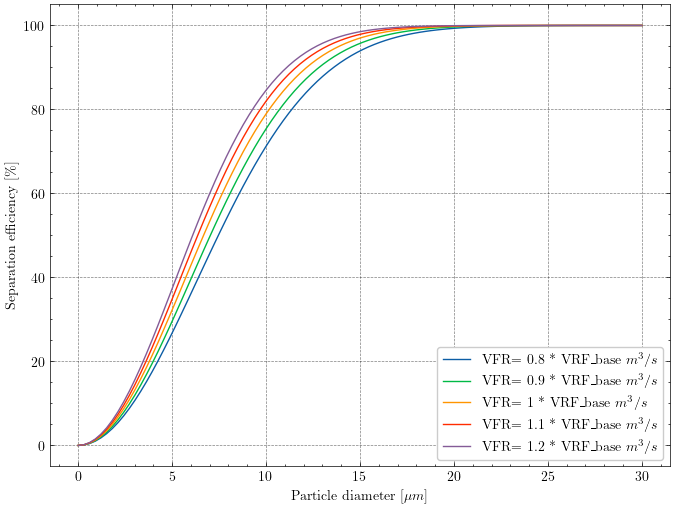
\includegraphics[width=1.0\linewidth]{images/efficiency_vs_inlet_VFR_porcent.png}
		\caption{}
		\label{inlet_VRF_porcent}
	\end{subfigure}
	\begin{subfigure}{.49\textwidth}
		\centering
		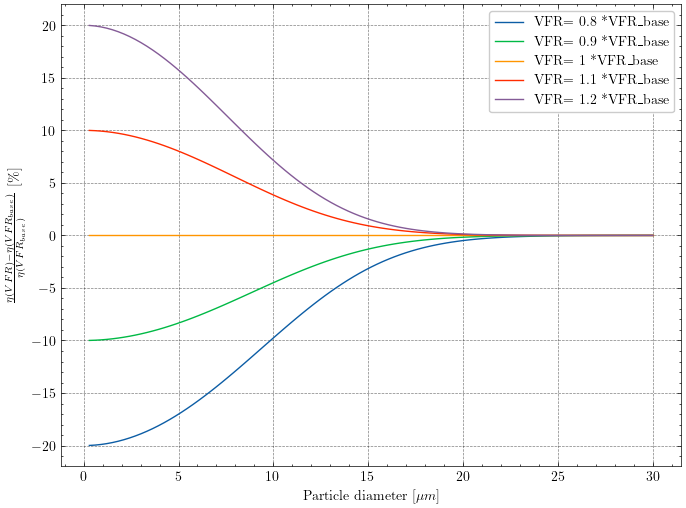
\includegraphics[width=1.0\linewidth]{images/efficiency_vs_inlet_VFR_relative.png}
		\caption{}
		\label{}
	\end{subfigure}
	\captionsetup{font=bf, size=small}
	\caption{ }
	\label{inlet_VRF_relative}
\end{figure}

Figure (\ref{inlet_VRF_relative}) shows  that the efficiency increases proportionally to the increase in VRF when the particle diameter is low. As the diameter of the particle increases, the effect of increasing VRF begins to decrease. However, it must be taken into account that the pressure loss varies with the square of the velocity in the inlet $\left(
\Delta p \propto v_{inlet} ^2 \right)$, so if the flow rate changes 10\% the pressure loss would increase by approximately 21\%.


%EN ALGUN LADO TENGO QUE PONER COMO SE CALCULA LA CONSTANTE KAPPA QUE ESTA RELACIONADA CON EL CAUDAL PARA QUE SE TERMINE DE ENTENDER ESTO.

%VER BIEN ESTA SECCION QUE QUEDO MEDIA FEA


\subsection{Optimization methodology}
In the previous section, the dimensions of a cyclone present in ref.\cite{Zhao2011} were used. That cyclone was used as a reference to see how the efficiency change for some parameters of interest such as temperature or flow rate, but said geometry was not optimal for the problem to be solved. For this reason, in this section the optimization process of the cyclone geometry is presented to maximize the separation efficiency, using both the fluid and the particle materials of interest for the problem.
\subsubsection{Geometrical optimization}

The next section presents how the optimization process was developed. For this, the Python library \texttt{Optimize} is used and \texttt{SLSQP} (Sequential Least Squares Programming) is used as the optimization method. In order to use this method, it is necessary to define the function to be minimized, the variables and both geometric and performance limitations.

In order to define the function, if a  target efficiency $\eta_{target}$ is defined , according to equation (\ref{efficiency_equation}) the radial velocity of the particle is

\begin{equation}
	v_{r,p}= - \frac{ln(1-\eta_{target})}{2 t_{res}} \cdot {R^*} _w
\end{equation}
On the other hand, using the equation (\ref{free_vortex_flow}), (\ref{effective_radious_equation}) and  (\ref{residence_time_equation})  the diameter of the particle can be expressed as:
\begin{align}
	d_p ^2 =&   \frac{18 \mu	v_{r,p}({R^*} _w) {R^*} _w}{\Delta \rho v_{\theta,f} ^2 ({R^*} _w)} \\
	d_p ^2 =&  - \frac{ln(1-\eta_{target})}{2 t_{res}} \cdot \frac{18 \mu {R^*} _w^2}{\Delta \rho v_{\theta,f}^2({R^*} _w) }\\
	d_p ^2 =&  - \frac{ln(1-\eta_{target})}{2 t_{res}} \cdot \frac{18 \mu {R^*} _w^{(2+2n)}}{\kappa^2 }
\end{align}
where the diameter of the particle is defined as a function of the target efficiency, inlet velocity (present in the parameter $\kappa$) and geometry (present in $t_{res}$, ${R^*}_w$ and $\kappa$). With this information, was used as a function to minimize,  the cut diameter defined as  the particle diameter for which the capture efficiency is equal to 50 \% $d_{p,c}=d_p(\eta=50 \%)$:
\begin{equation}
	d_{p.c} (\vec{x})  =  \left(  -  \frac{ln(0.5)}{2 t_{res}} \cdot \frac{18 \mu {R^*} _w^{(2+2n)}}{\kappa^2 }  \right)^{1/2}
\end{equation}

where $\vec{x}=(D,D_e,H,B,h,S,a,b)$ is the vector with all of geometrical variables of the cyclone.

In order to close the problem, the constrains used were:
\begin{enumerate}
	\item $h>S$
	\item $h>a$
	\item $D>D_e+b$
	\item $D_e>b$
	\item $H>S$
	\item $H>h$
	\item $D_e>B$
	\item $10$\textdegree $<\alpha<20$\textdegree , where $\alpha= arctan \left(  \frac{D-B}{2(H-h)} \right) $
	\item $v_{inlet} < v_{max}$
\end{enumerate}

Given that the problem has 8 variables  there are only inequalities as a constrains, more than one local minimum may exist within the domain. For this reason, the optimizer was  initialized with  different seeds in order to obtain the different local minima present in the domain.Then, a family of cyclones was obtained that meet the conditions within the domain, where the cutting diameter varies by less than 10\% and the geometric dimensions change. 



\subsubsection{Optimization: Results}
%(To do : find a better way to calculate the pressure loss throughout the cyclone).
%\begin{equation}
%	Q=\int_{A} v_{\theta,f}(r) dA= a \int_{r_1}^{r_2} \frac{\kappa}{r^n} dr
%\end{equation}
%\begin{equation}
%	\kappa=\frac{Q (1-n)}{a \left(r_2^{(1-n)}-r_1^{(1-n)} \right)}
%\end{equation}
%\begin{equation}
%	v_{\theta,f}(r)=\frac{Q (1-n)}{a  \left(r_2^{(1-n)}-r_1^{(1-n)}  \right)}  \frac{1}{r^n}
%\end{equation}

%Figure () present the the minimum 

%La figura () muestra el valor del diametro de corte en funcion del diametro optimo encontrado usando 256 semillas. se puede observar que a medida que aumenta la cantidad de cyclones en paralelo, el diametro del cyclone disminuye y disminuye considerablemente el diametro de corte. En el caso de utilizar solo un cyclone el diametro necesariamente tiene que ser muy grande para que la velocidad en el inlet no sea demasiado alta. 

%Ademas, la velocidad 

%el cyclone tiene que ser muy chico para poder tener una eficiencia muy alta a 1micro m.con solo un cyclone las dimensiones no son realistas.El cyclone puede servir para poder retirar impuresas de mayor tamano y despues es necesario utilizar algun otro sistema para poder retirar las particulas de menor tamano.

Table (\ref{input_VFR}) show the total volumetric mass flow rate for the commercial and pilot plant calculated in ref. \cite{power_scenario}. 

\begin{table}[H]
	\centering
	\begin{tabular}{ccc}
		\rule[-0.3cm]{0pt}{0.8cm}\textbf{Parameter}               & \textbf{Pilot plant} & \textbf{Commercial plant} \\ \hline
		\rule[-0.3cm]{0pt}{0.8cm}\textbf{VFR per loop {[}m3/s{]}} & 3.27                 & 4.9                       \\ \hline
		\rule[-0.3cm]{0pt}{0.8cm}\textbf{VFR total {[}m3/s{]}}    & 3.27                 & 29.4                     \\ \hline
	\end{tabular}
	\caption{Volumetric flow rate for the pilot and commercial plant calculated in ref. \cite{power_scenario}}
	\label{input_VFR}
\end{table}

For the optimization process, a parametric analysis was carried out where the VFR was varied in the inlet of the cyclone in order to have the same operating conditions in the cyclone for both the commercial and pilot plants and, consequently, the highest separation efficiency with the minimum loss of energy. The ratio between the VFR of the commercial plant and the pilot plant is approximately 9 $\left( \frac{(VFR_{total})_{commercial}}{(VFR_{total})_{pilot}} \approx 9 \right )$ so if you want to have the same efficiency for both plants, it is necessary to increase the number of cyclones 9 times when scaling the plant from the pilot to the commercial one.

%On the other hand, another possible alternative if the maximum number of cyclones for the commercial plant is limited, either due to economic cost or space limitations, etc., figure () shows the sensitivity of the efficiency when varying the VFR inlet in the cyclone. 

Figure (\ref{Fe_d_cut_off}) ,(\ref{Cr_d_cut_off}) and (\ref{AlN_d_cut_off}) shows the cut off diameter ($\eta=50\%$)  for the Fe, Cr and AlN, respectively.  For this analysis, it has been used that the maximum velocity in the inlet has to be less than 25 m/s.

\begin{figure}[H]
	\centering
	\begin{subfigure}{.49\textwidth}
		\centering
		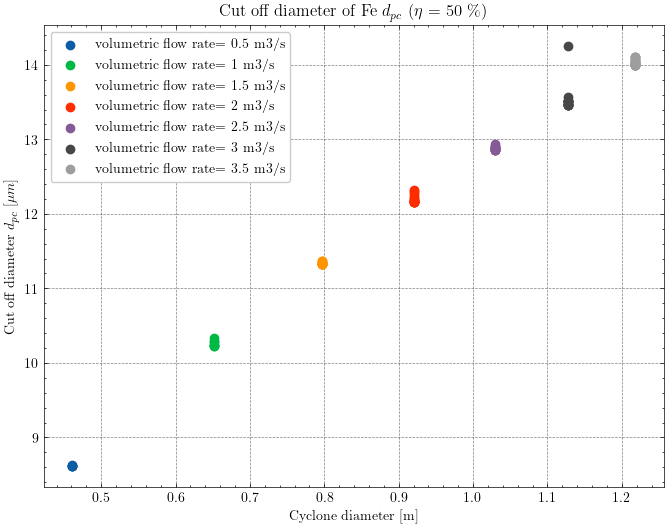
\includegraphics[width=1.0\linewidth]{images/d_pc_Fe.png}
		\caption{}
		\label{Fe_d_cut_off}
	\end{subfigure}
	\begin{subfigure}{.49\textwidth}
		\centering
		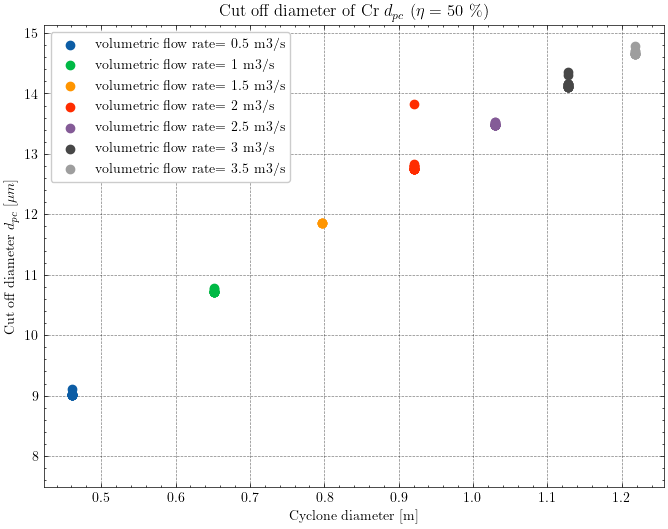
\includegraphics[width=1.0\linewidth]{images/d_pc_Cr.png}
		\caption{}
		\label{Cr_d_cut_off}
	\end{subfigure}
	\begin{subfigure}{.49\textwidth}
		\centering
		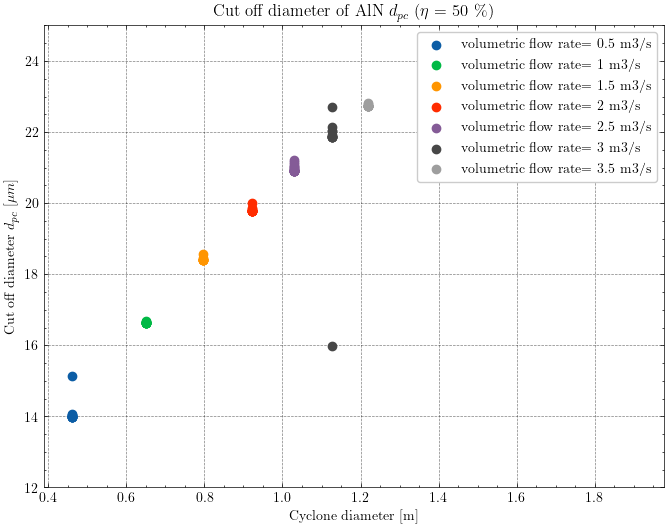
\includegraphics[width=1.0\linewidth]{images/d_pc_AlN.png}
		\caption{}
		\label{AlN_d_cut_off}
	\end{subfigure}
	\captionsetup{font=bf, size=small}
	\caption{ }
	\label{}
\end{figure}

It can be seen that the cutting diameter of both Fe and Cr are quite similar and smaller than that of AlN. This is because the density of Fe is similar to that of Cr, while the density of AlN is much lower. This causes the radial velocity of the particle towards the walls to be lower and the efficiency tends to decrease, so the diameter of the particle must be larger to be captured.

Since the inlet maximum velocity was limited in the optimization process, when the volumetric flow rate increase the cyclone diameter and the inlet dimensions have to grow to have enough space to allocate the inlet and reduce the velocity.    

Table (\ref{info_cyclone}) presents the dimensions of 5 cyclones that can operate at different VFRs. In addition, the cutting diameter for Fe, Cr and AlN is presented and an estimate of the number of cyclones that could be used either in the commercial plant or in the pilot plant.
\begin{table}[H]
	\begin{tabular}{cccccc}
		\rule[-0.3cm]{0pt}{0.8cm}\textbf{Cyclone   case}                                        & \textbf{I} & \textbf{II} & \textbf{III} & \textbf{IV} & \textbf{V} \\ \hline
		\rule[-0.3cm]{0pt}{0.8cm}\textbf{Cyclone body diameter (m)}                             & 0.460      & 0.651       & 0.797        & 0.921       & 1.030      \\\hline
		\rule[-0.3cm]{0pt}{0.8cm}\textbf{Liquid outlet diameter (vortex finder diameter) (m)} & 0.211      & 0.291       & 0.357        & 0.412       & 0.461      \\\hline
		\rule[-0.3cm]{0pt}{0.8cm}\textbf{Cyclone inlet height (m)}                               & 0.230      & 0.326       & 0.399        & 0.460       & 0.515      \\\hline
		\rule[-0.3cm]{0pt}{0.8cm}\textbf{Cyclone inlet width (m)}                          & 0.092      & 0.130       & 0.159        & 0.184       & 0.206      \\\hline
		\rule[-0.3cm]{0pt}{0.8cm}\textbf{Liquid outlet duct length (m)}                         & 0.436      & 0.620       & 0.760        & 0.877       & 0.981      \\\hline
		\rule[-0.3cm]{0pt}{0.8cm}\textbf{Cyclone cylinder height (m)}                           & 1.483      & 2.063       & 2.526        & 2.917       & 3.261      \\\hline
		\rule[-0.3cm]{0pt}{0.8cm}\textbf{Cyclone height (m)}                                    & 0.460      & 0.651       & 0.797        & 0.921       & 1.030      \\\hline
		\rule[-0.3cm]{0pt}{0.8cm}\textbf{Particle outlet diameter (m)}                          & 0.046      & 0.065       & 0.080        & 0.092       & 0.103      \\\hline
		\rule[-0.3cm]{0pt}{0.8cm}\textbf{Angle ($^{\circ}$)}                                                 & 11.453     & 11.723      & 11.732       & 11.731      & 11.731     \\\hline
		\rule[-0.3cm]{0pt}{0.8cm}\textbf{Inlet VFR (m3/s)}                                      & 0.5     & 1.0       & 1.5       & 2.0       & 2.5      \\\hline
		\rule[-0.3cm]{0pt}{0.8cm}\textbf{Inlet Velocity (m/s)}                                        & 23.585     & 23.585      & 23.585       & 23.585      & 23.585     \\\hline
		\rule[-0.3cm]{0pt}{0.8cm}\textbf{Cut off diameter Fe (microns)}                         & 8.610      & 10.230      & 11.322       & 12.053      & 12.864     \\\hline
		\rule[-0.3cm]{0pt}{0.8cm}\textbf{Cut off diameter Cr  (microns)}                        & 9.013      & 10.468      & 11.861       & 12.746      & 13.477     \\\hline
		\rule[-0.3cm]{0pt}{0.8cm}\textbf{Cut off diameter AlN (microns)}                        & 10.207     & 16.620      & 18.393       & 19.765      & 21.215     \\\hline
		\rule[-0.3cm]{0pt}{0.8cm}\textbf{Number of cyclone pilot   plant}                       & 6          & 3           & 2            &             &            \\\hline
		\rule[-0.3cm]{0pt}{0.8cm}\textbf{Number of cyclone commercial plant}                  & 54         & 27          & 18           &             &              \\\hline
	\end{tabular}
	\caption{Cyclone optimization results}
	\label{info_cyclone}
\end{table}


It can be seen that as the volumetric flow rate at the inlet increases, the cut off diameter decrease for all the particles analyzed, causing the lose of separation efficiency. On the other hand, in order to  choose the correct cyclone,the total pressure loss of the system have to be considered. In the literature there are a large number of correlations to calculate pressure loss \cite{Concha2007,Altmeyer2003}, however these are developed mainly for gas-solid cyclones and not for liquid-solid as in this case. For this reason, in the CFD section, importance will be given to the calculation of said parameter.



%\begin{figure}[H]
%	\centering
%	\begin{subfigure}{.49\textwidth}
%		\centering
%		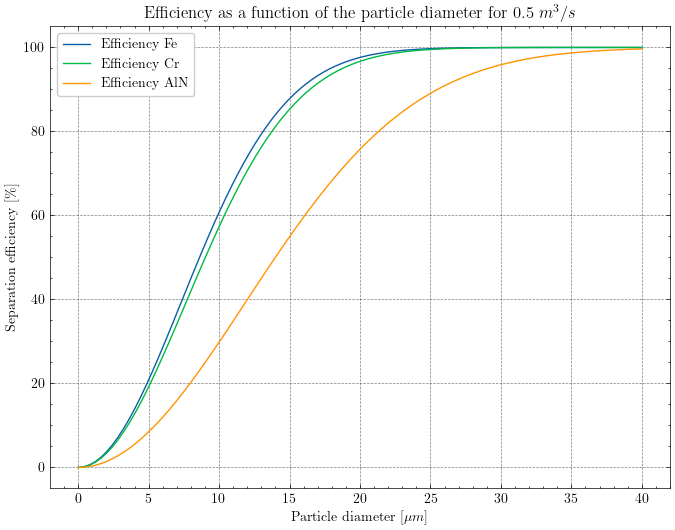
\includegraphics[width=1.0\linewidth]{images/efficiency_for_0.5m3_s.png}
%		\caption{}
%		\label{}
%	\end{subfigure}
%	\begin{subfigure}{.49\textwidth}
%		\centering
%		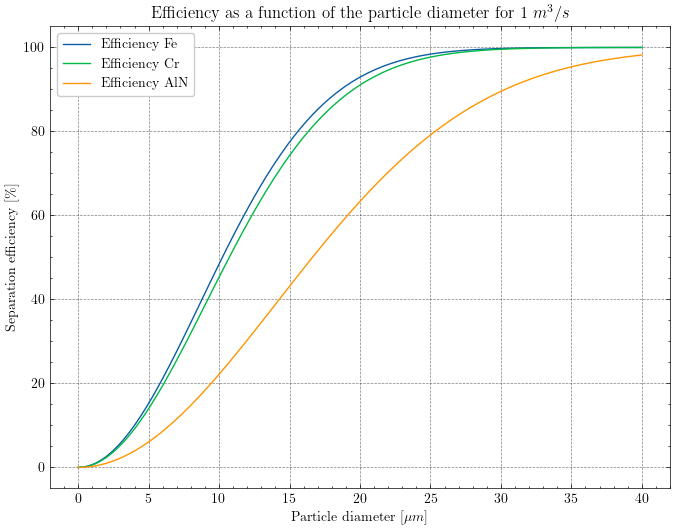
\includegraphics[width=1.0\linewidth]{images/efficiency_for_1m3_s.png}
%		\caption{}
%		\label{}
%	\end{subfigure}
%	\begin{subfigure}{.49\textwidth}
%		\centering
%		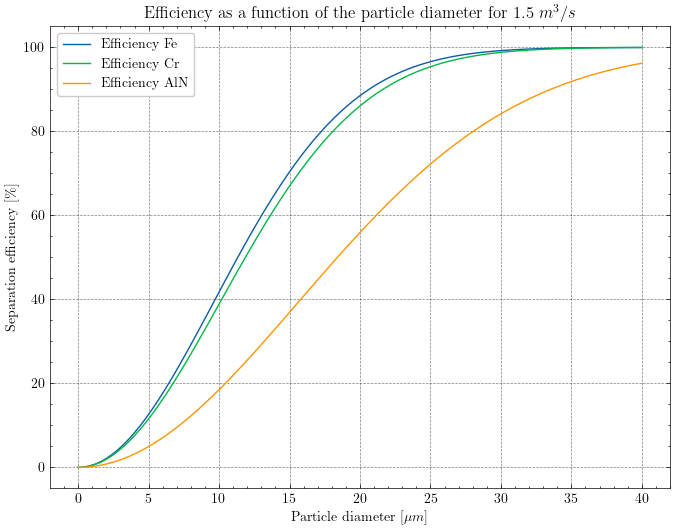
\includegraphics[width=1.0\linewidth]{images/efficiency_for_1.5m3_s.png}
%		\caption{}
%		\label{}
%	\end{subfigure}
%	\captionsetup{font=bf, size=small}
%	\caption{ }
%	\label{}
%\end{figure}





\newpage
\subsection{Conceptual Design Approach}
In the forthcoming project phases, the conceptual design will navigate the design space between the hydrocyclone and Disk Stack Separator, aiming to optimize the multi-stage purification process. With the requirements outlined in Section \ref{sec:sss} and the technical specifications detailed in Figure \ref{multi_stage_technical} serving as foundational guidelines, the design endeavor will seek to exploit the current capabilities of the multi-stage purification system. Drawing inspiration from external sources, such as referenced paper ref. \cite{Van}, the conceptual design will explore innovative approaches (Figure \ref{design_conceptual}) to enhance particle capture efficiency, impurity removal, and overall system performance.\\


\noindent Integration of advanced materials, novel geometries, and optimized operational parameters will be central to the conceptual design exploration. By leveraging insights from existing research and technological advancements, the conceptual design aims to push the boundaries of purification efficiency, ultimately culminating in the development of a device that maximizes the potential of the multi-stage purification process. 


\begin{figure}[H]
	\centering
	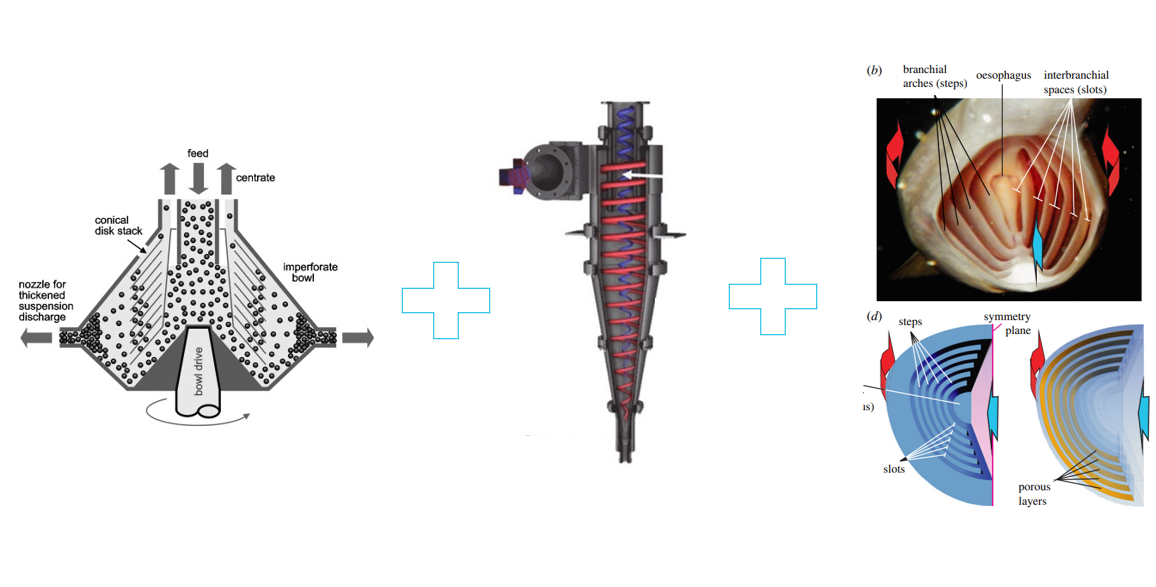
\includegraphics[width=1\linewidth]{design_conceptual.png}
	\captionsetup{font=bf, size=small}
	\caption{Conceptual design approach: possible lines of work}
	\label{design_conceptual}
\end{figure}



\newpage

\section{CONCLUSIONS}








 
xxxxxxxxxxxxxxxxxxxxxxxxxxxxxxxxxxxxxxxxxxxxxxxxxxxxxxxxxxxxxxxxxx





